\section{Resultados}

\subsection{Sensibilidade quanto ao número de amostras}

%Samples%
\begin{figure}[!ht]
	\centering
	\caption{Número de pontos amostrais no espaço de fases definido por $\sigma \times \partial_{x} u$.}
	\begin{subfigure}[b]{0.45\linewidth}
		\centering
		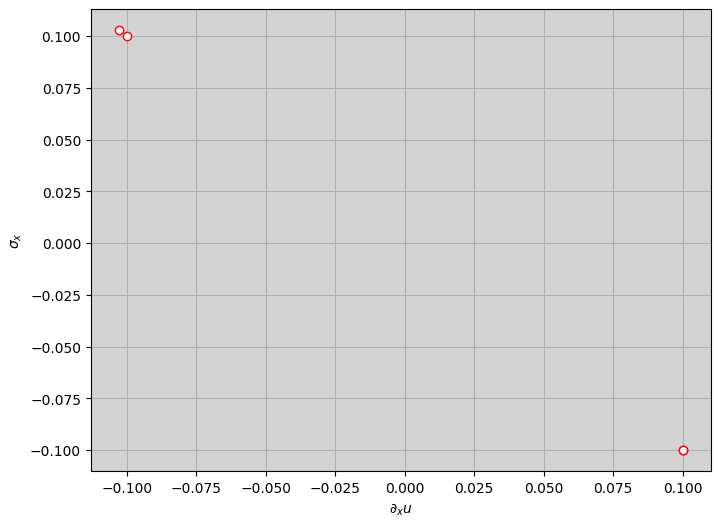
\includegraphics[width = 1.0\linewidth]{Figuras/Sensibilidade_amostras/Nxy_sample_2_2.png}
		\caption{$\text{N}_{x}^{\text{amostras}} = \text{N}_{y}^{\text{amostras}} = 2$.}
		\label{fig:Nxy_sample_2_2}
	\end{subfigure}
	\hfill
	\begin{subfigure}[b]{0.45\linewidth}
		\centering
		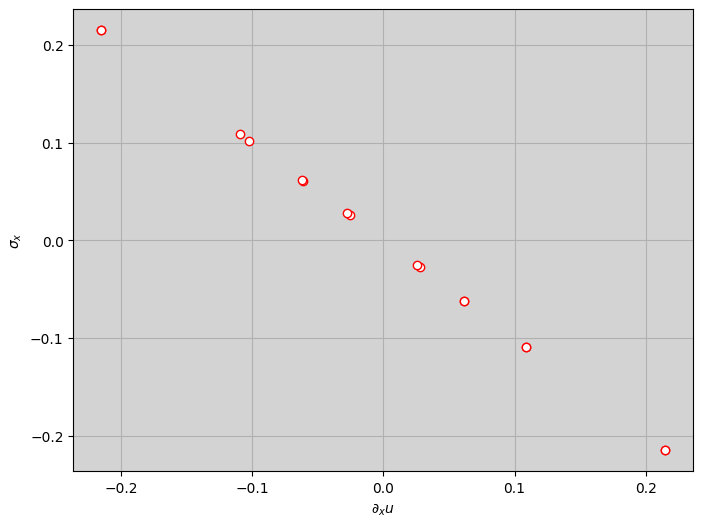
\includegraphics[width = 1.0\linewidth]{Figuras/Sensibilidade_amostras/Nxy_sample_4_4.png}
		\caption{$\text{N}_{x}^{\text{amostras}} = \text{N}_{y}^{\text{amostras}} = 4$.}
		\label{fig:Nxy_sample_4_4}
	\end{subfigure}
	\hfill
	\begin{subfigure}[b]{0.45\linewidth}
		\centering
		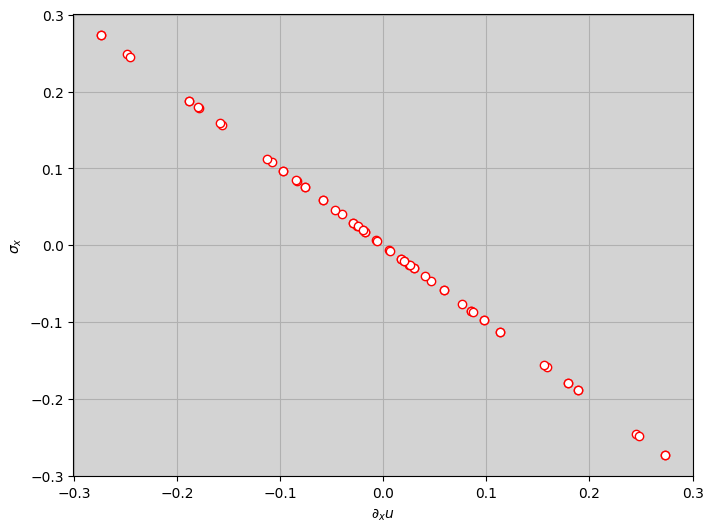
\includegraphics[width = 1.0\linewidth]{Figuras/Sensibilidade_amostras/Nxy_sample_8_8.png}
		\caption{$\text{N}_{x}^{\text{amostras}} = \text{N}_{y}^{\text{amostras}} = 8$.}
		\label{fig:Nxy_sample_8_8}
	\end{subfigure}
	\hfill
	\begin{subfigure}[b]{0.45\linewidth}
		\centering
		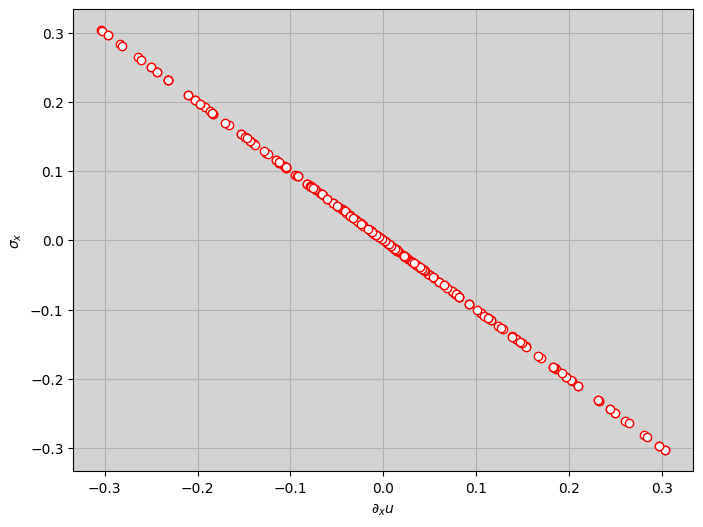
\includegraphics[width = 1.0\linewidth]{Figuras/Sensibilidade_amostras/Nxy_sample_16_16.png}
		\caption{$\text{N}_{x}^{\text{amostras}} = \text{N}_{y}^{\text{amostras}} = 16$.}
		\label{fig:Nxy_sample_16_16}
	\end{subfigure}
	\label{fig:Nxy_sample}
\end{figure}

%Pressure%
\begin{figure}[!ht]
	\centering
	\caption{À esquerda, curvas de nível do campo escalar de pressões, $p$, considerando os números de pontos amostrais retratados nas figuras \ref{fig:Nxy_sample_2_2} e \ref{fig:Nxy_sample_4_4}. À direita, as respectivas representações tridimensionais.}
	\begin{subfigure}[b]{0.45\linewidth}
		\centering
		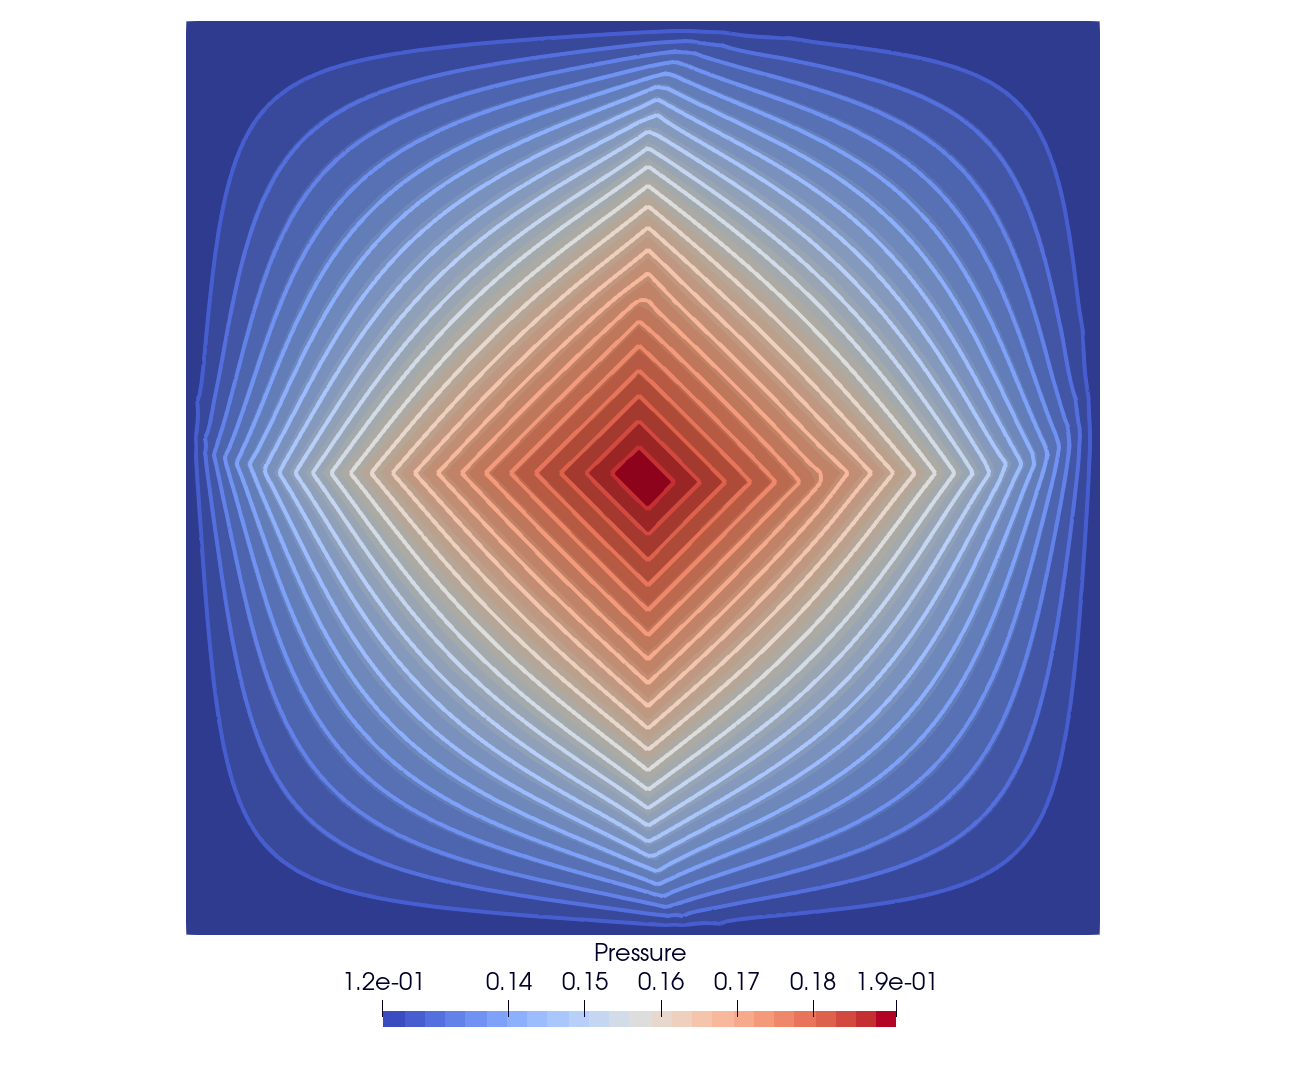
\includegraphics[width = 1.0\linewidth]{Figuras/Sensibilidade_amostras/pressure_contour_NxNy101_Nsample2_2.png}
		\caption{$\text{N}_{x}^{\text{amostras}} = \text{N}_{y}^{\text{amostras}} = 2$.}
		\label{fig:pressure_contour_NxNy101_Nsample2_2}
	\end{subfigure}
	\hfill
	\begin{subfigure}[b]{0.45\linewidth}
		\centering
		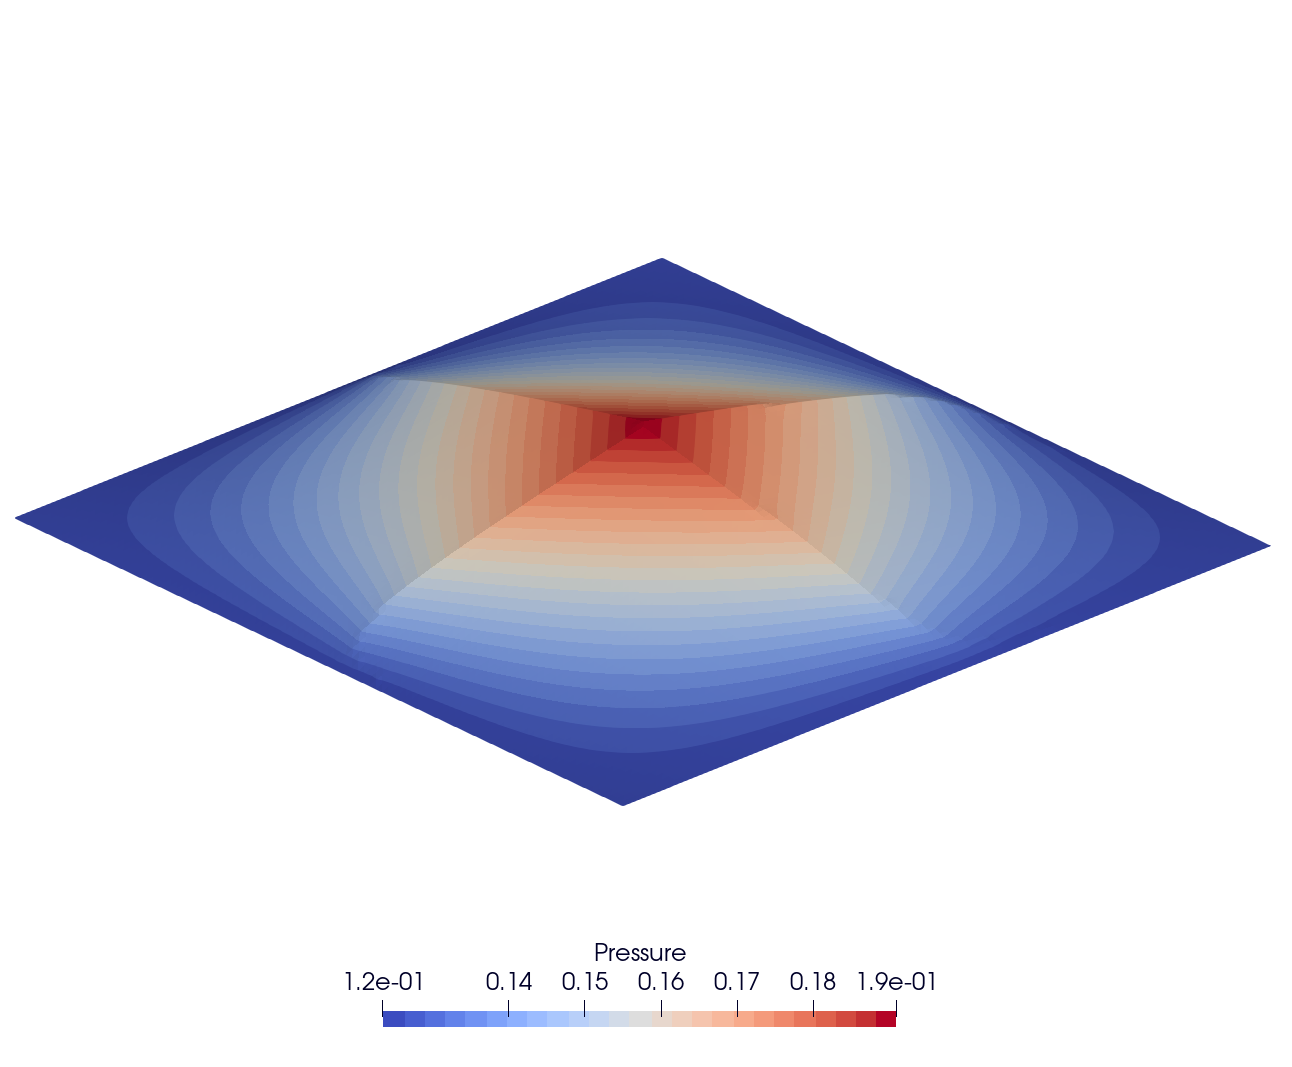
\includegraphics[width = 1.0\linewidth]{Figuras/Sensibilidade_amostras/pressure_wrapesc_NxNy101_Nsample2_2.png}
		\caption{$\text{N}_{x}^{\text{amostras}} = \text{N}_{y}^{\text{amostras}} = 2$.}
		\label{fig:pressure_wrapesc_NxNy101_Nsample2_2}
	\end{subfigure}
	\hfill
	\begin{subfigure}[b]{0.45\linewidth}
		\centering
		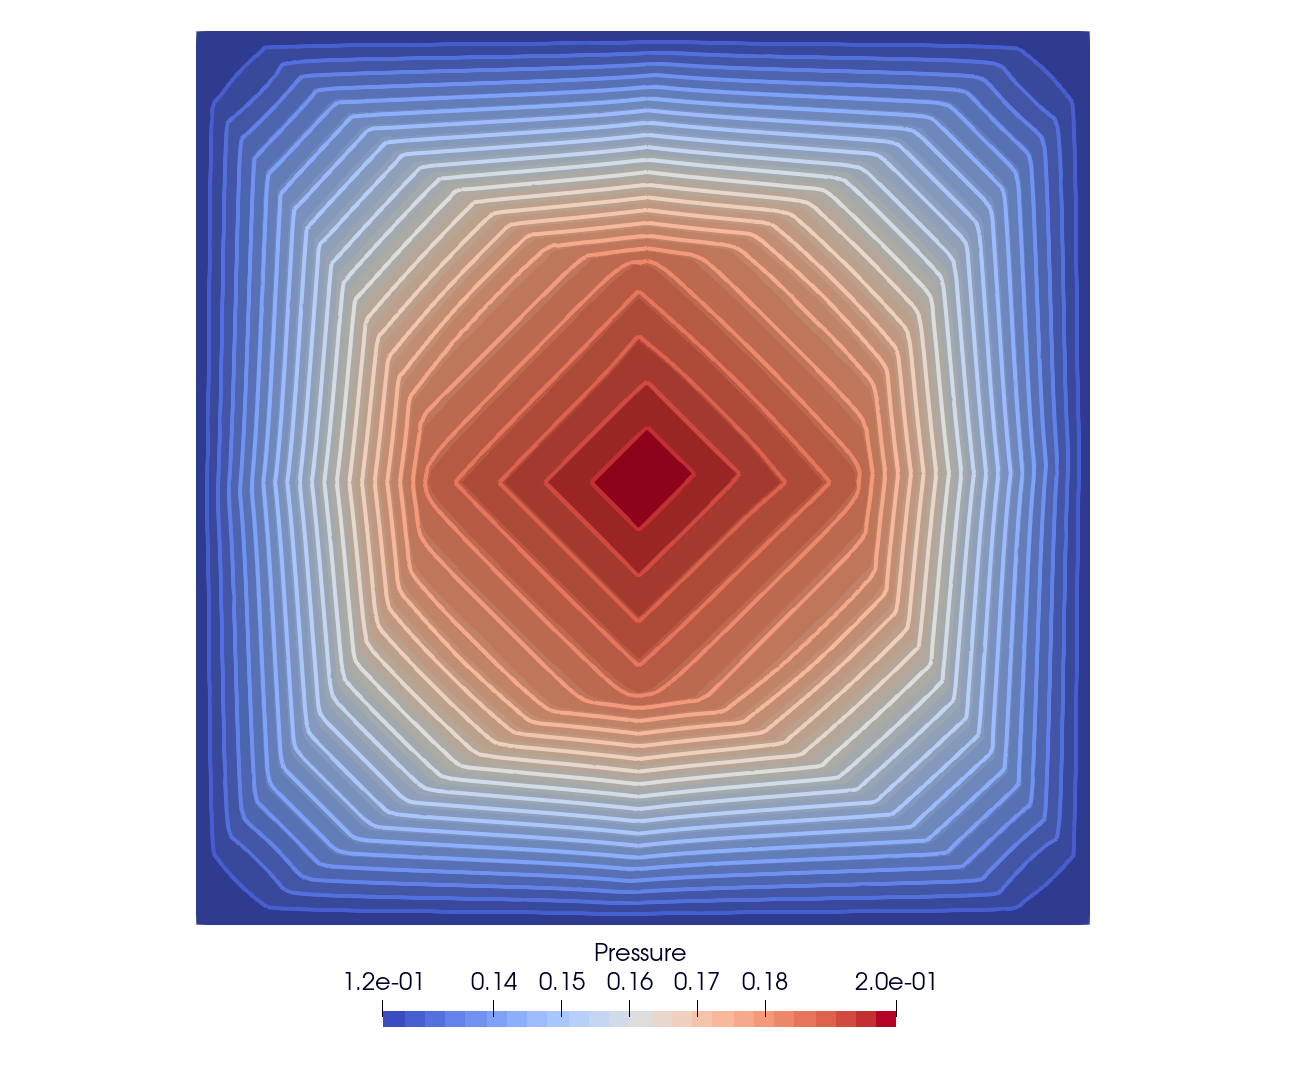
\includegraphics[width = 1.0\linewidth]{Figuras/Sensibilidade_amostras/pressure_contour_NxNy101_Nsample4_4.png}
		\caption{$\text{N}_{x}^{\text{amostras}} = \text{N}_{y}^{\text{amostras}} = 4$.}
		\label{fig:pressure_contour_NxNy101_Nsample4_4}
	\end{subfigure}
	\hfill
	\begin{subfigure}[b]{0.45\linewidth}
		\centering
		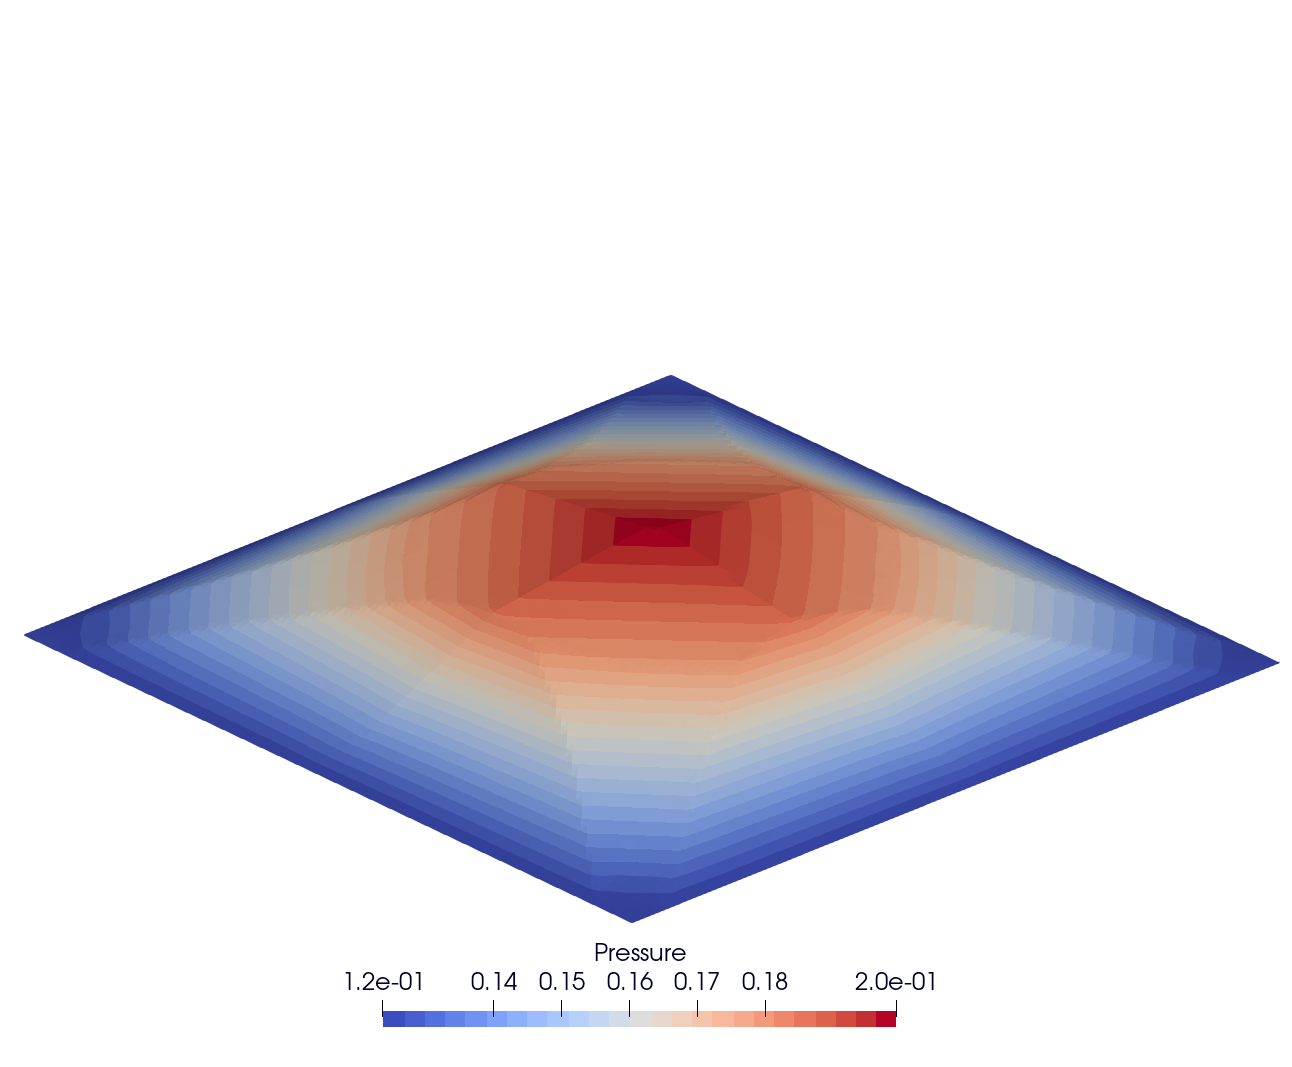
\includegraphics[width = 1.0\linewidth]{Figuras/Sensibilidade_amostras/pressure_wrapesc_NxNy101_Nsample4_4.png}
		\caption{$\text{N}_{x}^{\text{amostras}} = \text{N}_{y}^{\text{amostras}} = 4$.}
		\label{fig:pressure_wrapesc_NxNy101_Nsample4_4}
	\end{subfigure}
	\label{fig:pressure_sample_low_values}
\end{figure}


\begin{figure}[!ht]
	\centering
	\caption{À esquerda, curvas de nível do campo escalar de pressões, $p$, considerando os números de pontos amostrais retratados nas figuras \ref{fig:Nxy_sample_8_8} e \ref{fig:Nxy_sample_16_16}. À direita, as respectivas representações tridimensionais.}
	\begin{subfigure}[b]{0.45\linewidth}
		\centering
		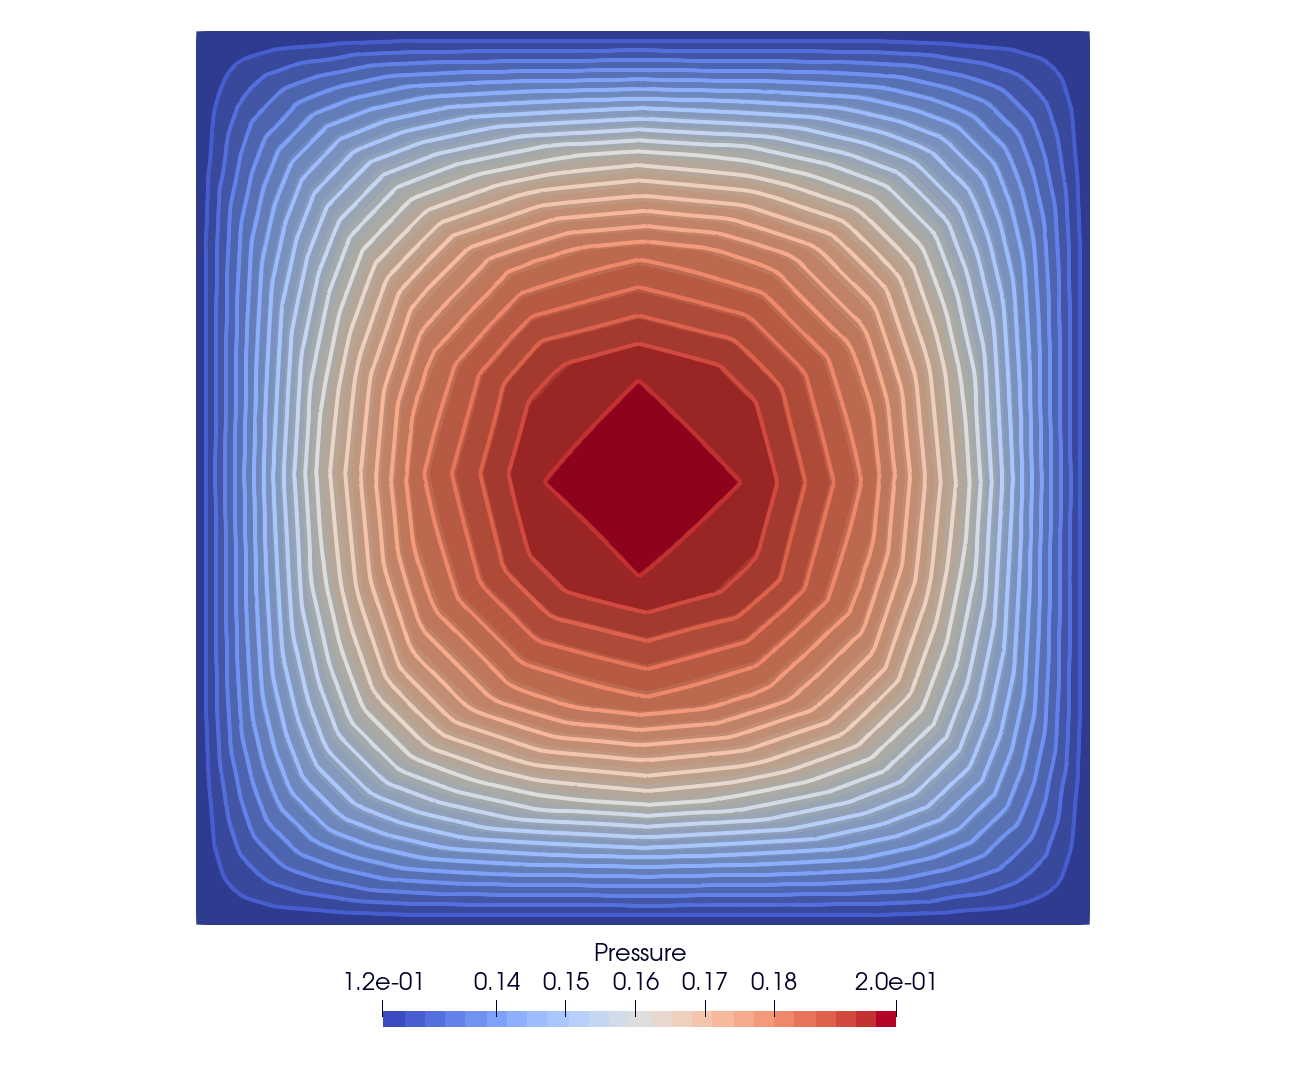
\includegraphics[width = 1.0\linewidth]{Figuras/Sensibilidade_amostras/pressure_contour_NxNy101_Nsample8_8.png}
		\caption{$\text{N}_{x}^{\text{amostras}} = \text{N}_{y}^{\text{amostras}} = 8$.}
		\label{fig:pressure_contour_NxNy101_Nsample8_8}
	\end{subfigure}
	\hfill
	\begin{subfigure}[b]{0.45\linewidth}
		\centering
		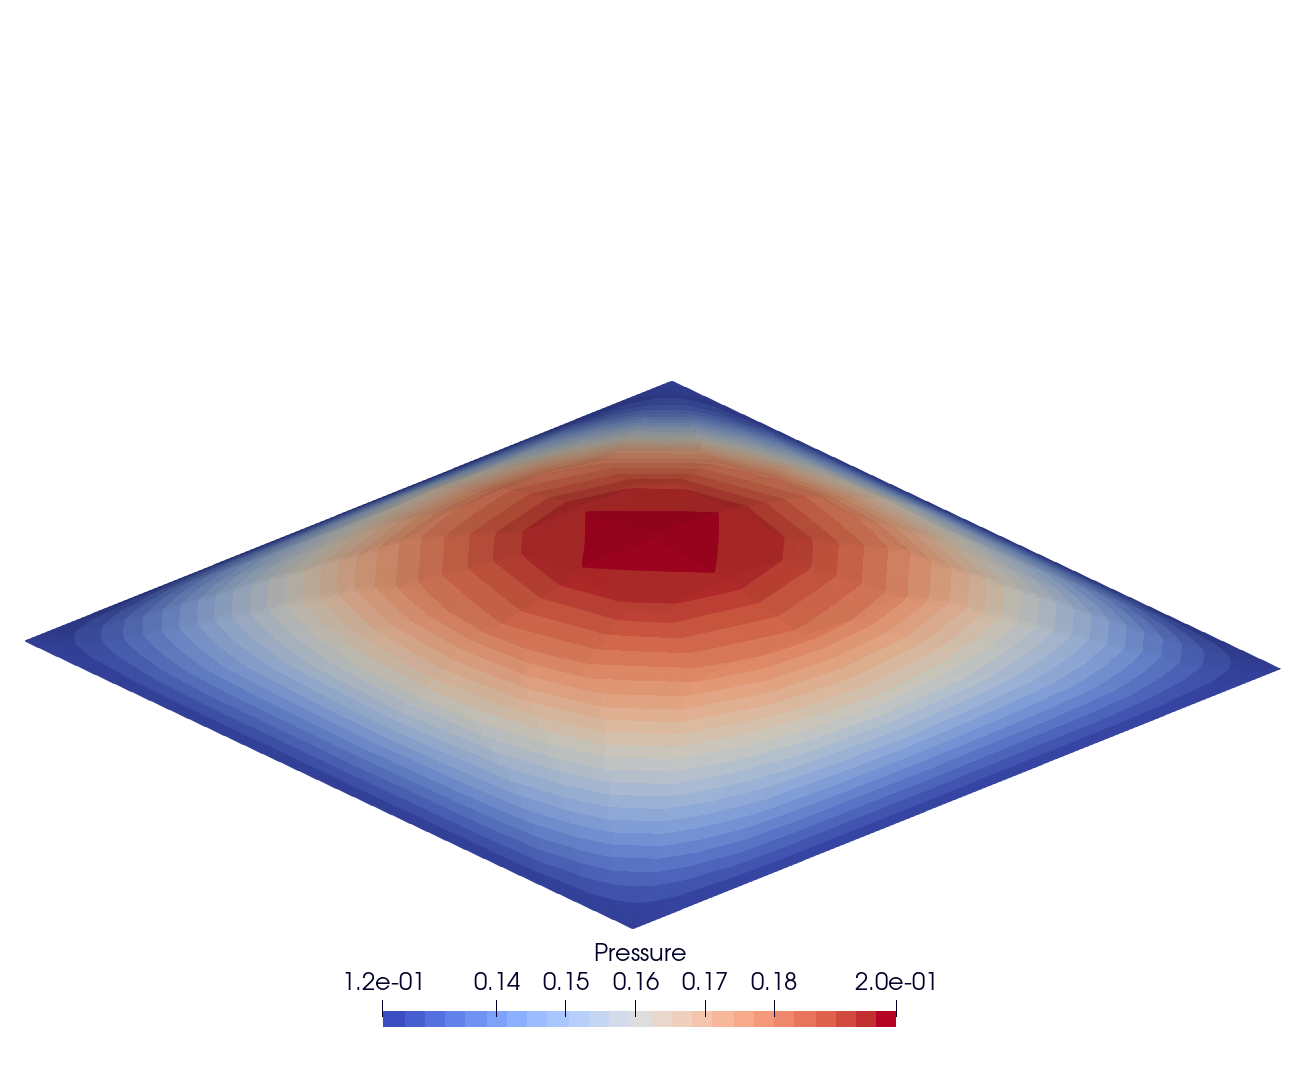
\includegraphics[width = 1.0\linewidth]{Figuras/Sensibilidade_amostras/pressure_wrapesc_NxNy101_Nsample8_8.png}
		\caption{$\text{N}_{x}^{\text{amostras}} = \text{N}_{y}^{\text{amostras}} = 8$.}
		\label{fig:pressure_wrapesc_NxNy101_Nsample8_8}
	\end{subfigure}
	\hfill
	\begin{subfigure}[b]{0.45\linewidth}
		\centering
		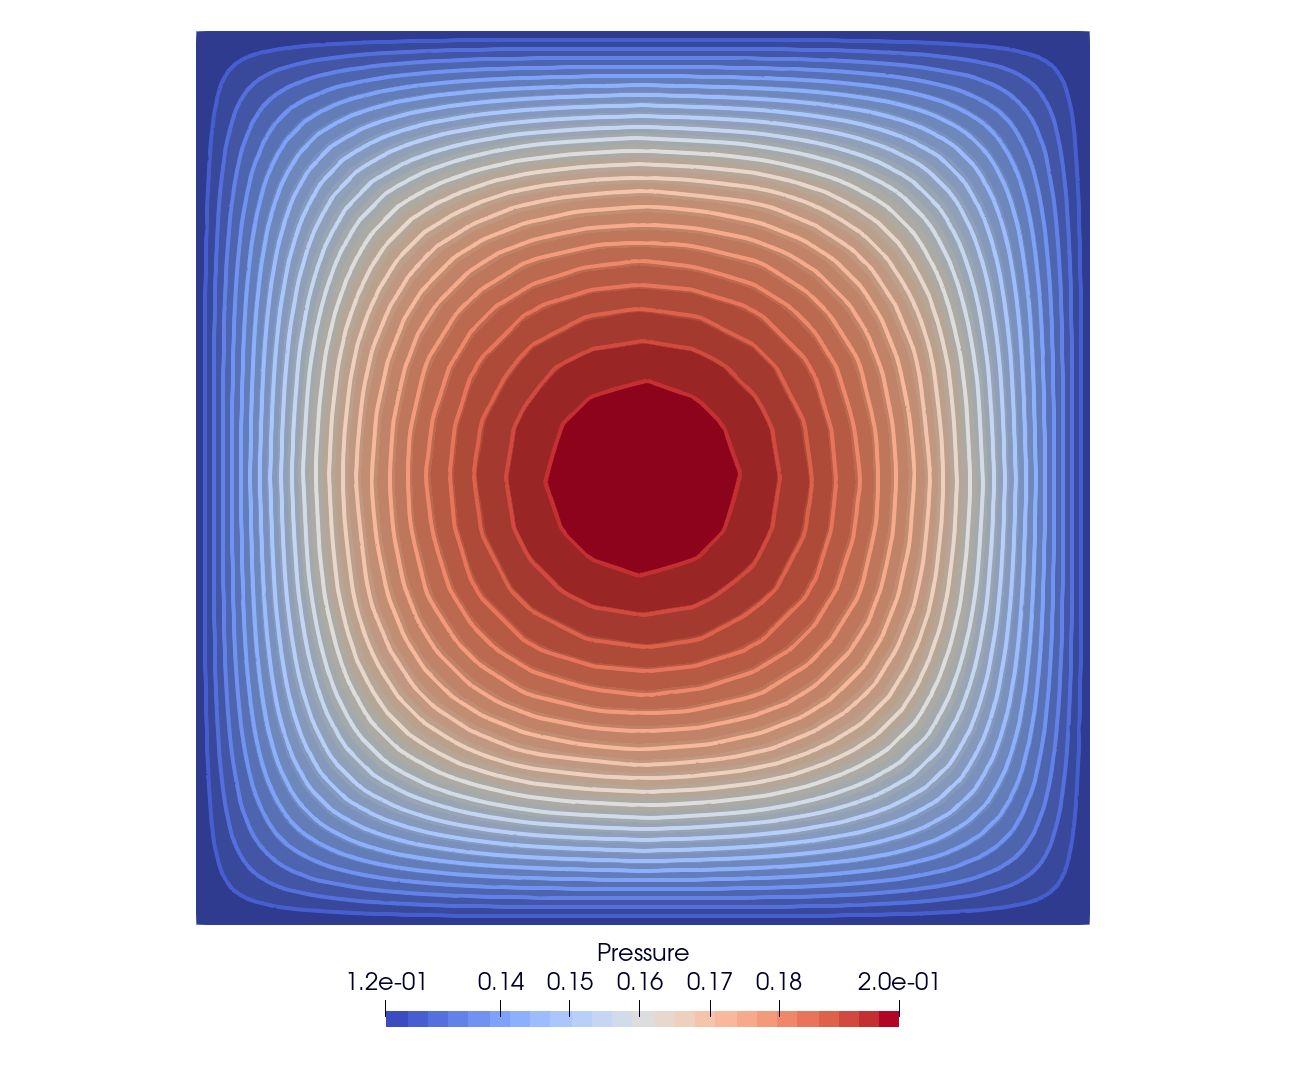
\includegraphics[width = 1.0\linewidth]{Figuras/Sensibilidade_amostras/pressure_contour_NxNy101_Nsample16_16.png}
		\caption{$\text{N}_{x}^{\text{amostras}} = \text{N}_{y}^{\text{amostras}} = 16$.}
		\label{fig:pressure_contour_NxNy101_Nsample16_16}
	\end{subfigure}
	\hfill
	\begin{subfigure}[b]{0.45\linewidth}
		\centering
		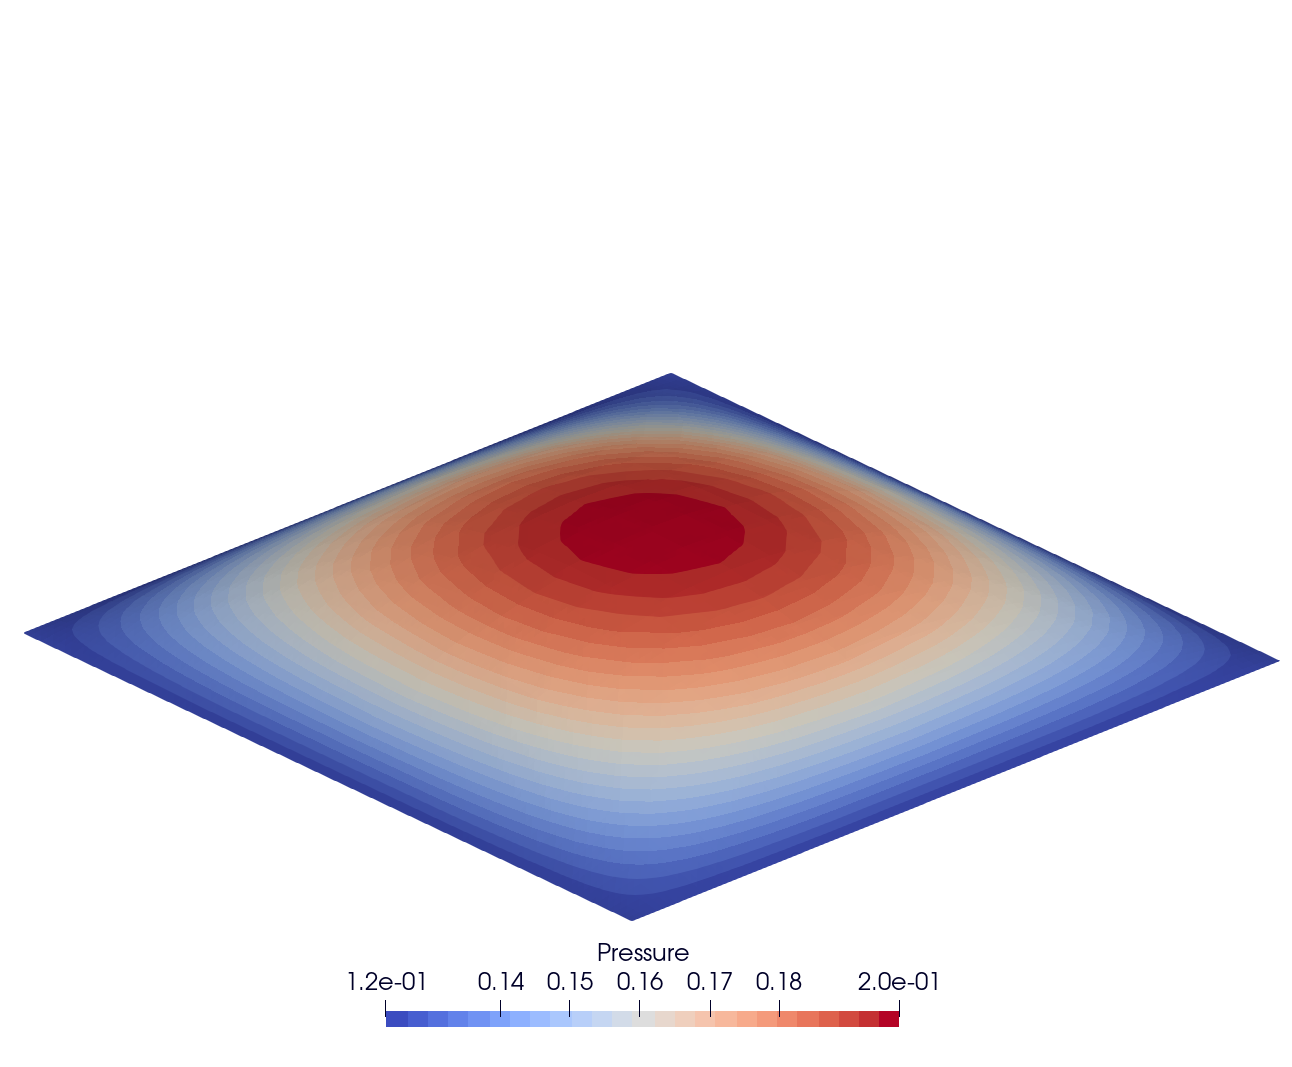
\includegraphics[width = 1.0\linewidth]{Figuras/Sensibilidade_amostras/pressure_wrapesc_NxNy101_Nsample16_16.png}
		\caption{$\text{N}_{x}^{\text{amostras}} = \text{N}_{y}^{\text{amostras}} = 16$.}
		\label{fig:pressure_wrapesc_NxNy101_Nsample16_16}
	\end{subfigure}
	\label{fig:pressure_sample_high_values}
\end{figure}

%lambda%
\begin{figure}[!ht]
	\centering
	\caption{À esquerda, curvas de nível do campo escalar de multiplicadores de Lagrange considerando os números de pontos amostrais retratados nas figuras \ref{fig:Nxy_sample_2_2} e \ref{fig:Nxy_sample_4_4}. À direita, as respectivas representações tridimensionais.}
	\begin{subfigure}[b]{0.45\linewidth}
		\centering
		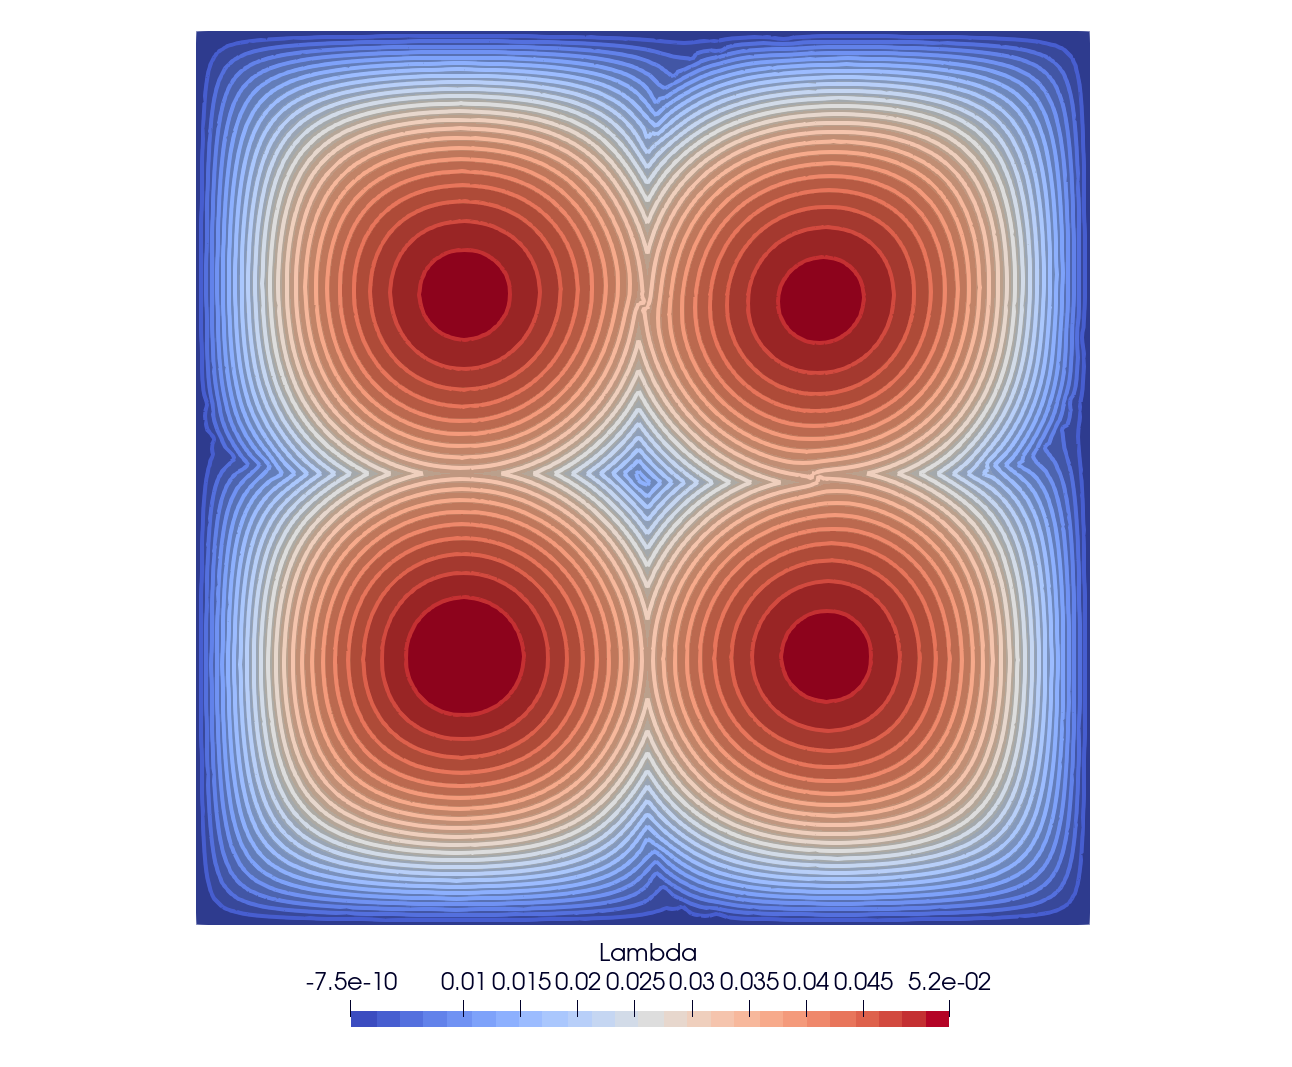
\includegraphics[width = 1.0\linewidth]{Figuras/Sensibilidade_amostras/lambda_contour_NxNy101_Nsample2_2.png}
		\caption{$\text{N}_{x}^{\text{amostras}} = \text{N}_{y}^{\text{amostras}} = 2$.}
		\label{fig:lambda_contour_NxNy101_Nsample2_2}
	\end{subfigure}
	\hfill
	\begin{subfigure}[b]{0.45\linewidth}
		\centering
		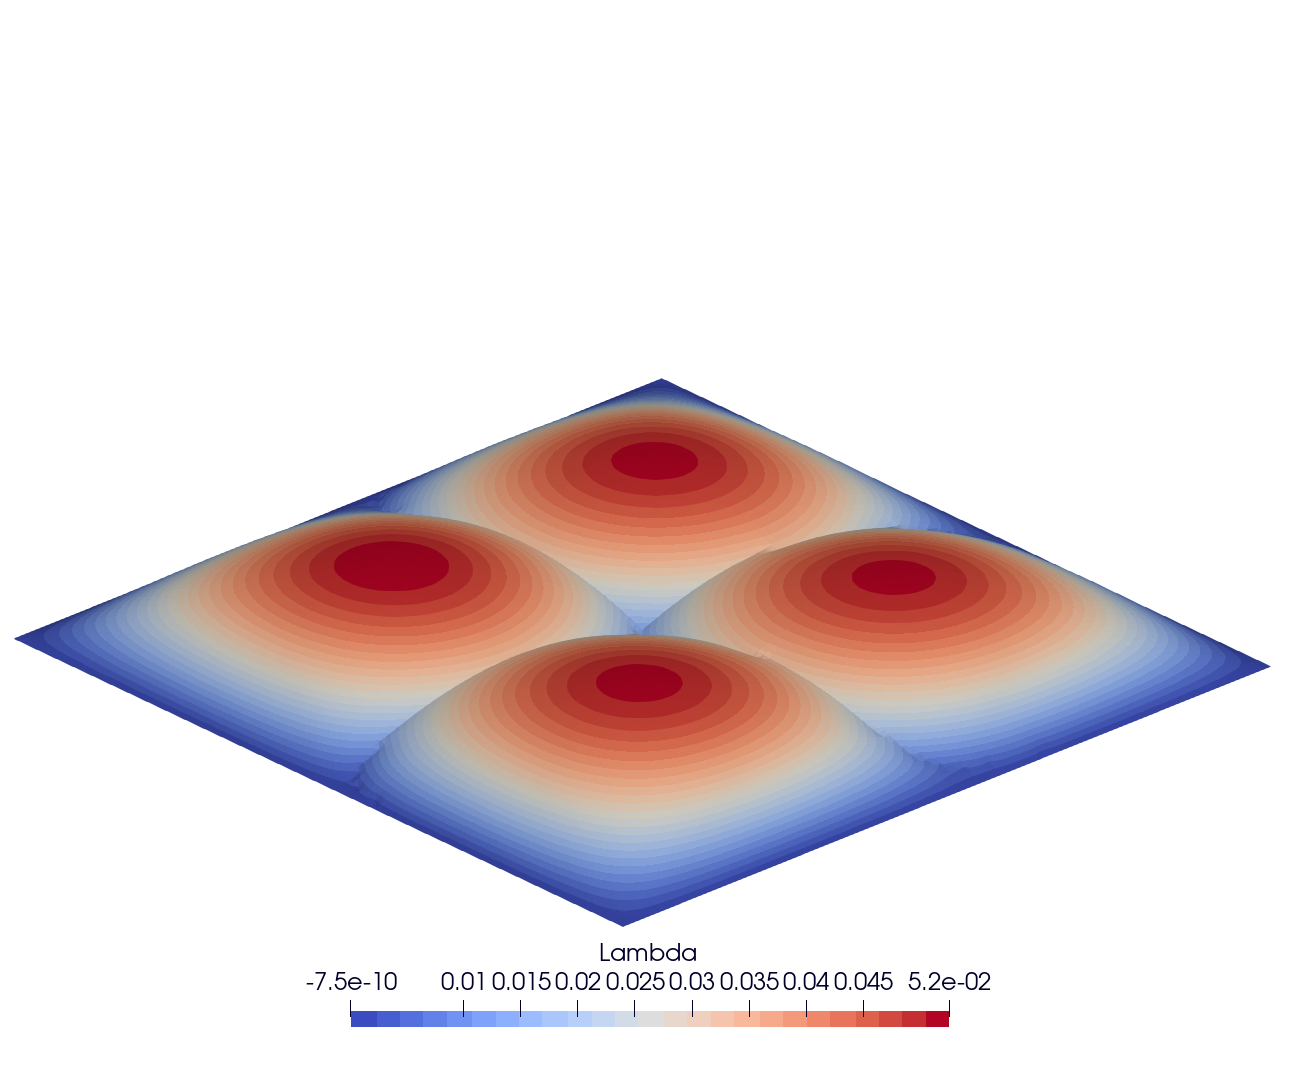
\includegraphics[width = 1.0\linewidth]{Figuras/Sensibilidade_amostras/lambda_wrapesc_NxNy101_Nsample2_2.png}
		\caption{$\text{N}_{x}^{\text{amostras}} = \text{N}_{y}^{\text{amostras}} = 2$.}
		\label{fig:lambda_wrapesc_NxNy101_Nsample2_2}
	\end{subfigure}
	\hfill
	\begin{subfigure}[b]{0.45\linewidth}
		\centering
		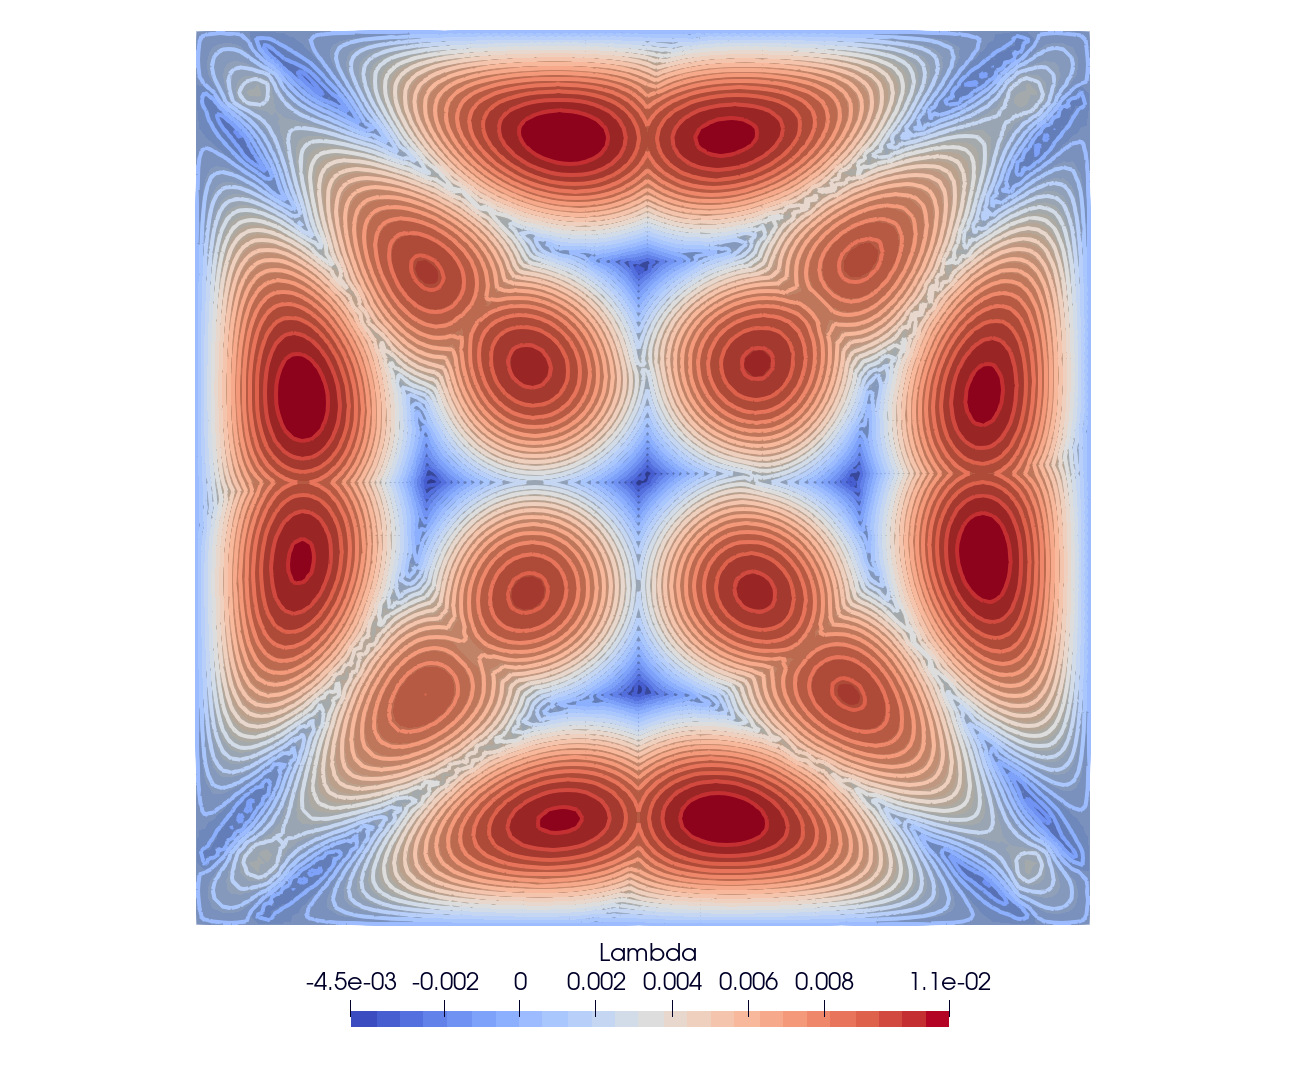
\includegraphics[width = 1.0\linewidth]{Figuras/Sensibilidade_amostras/lambda_contour_NxNy101_Nsample4_4.png}
		\caption{$\text{N}_{x}^{\text{amostras}} = \text{N}_{y}^{\text{amostras}} = 4$.}
		\label{fig:lambda_contour_NxNy101_Nsample4_4}
	\end{subfigure}
	\hfill
	\begin{subfigure}[b]{0.45\linewidth}
		\centering
		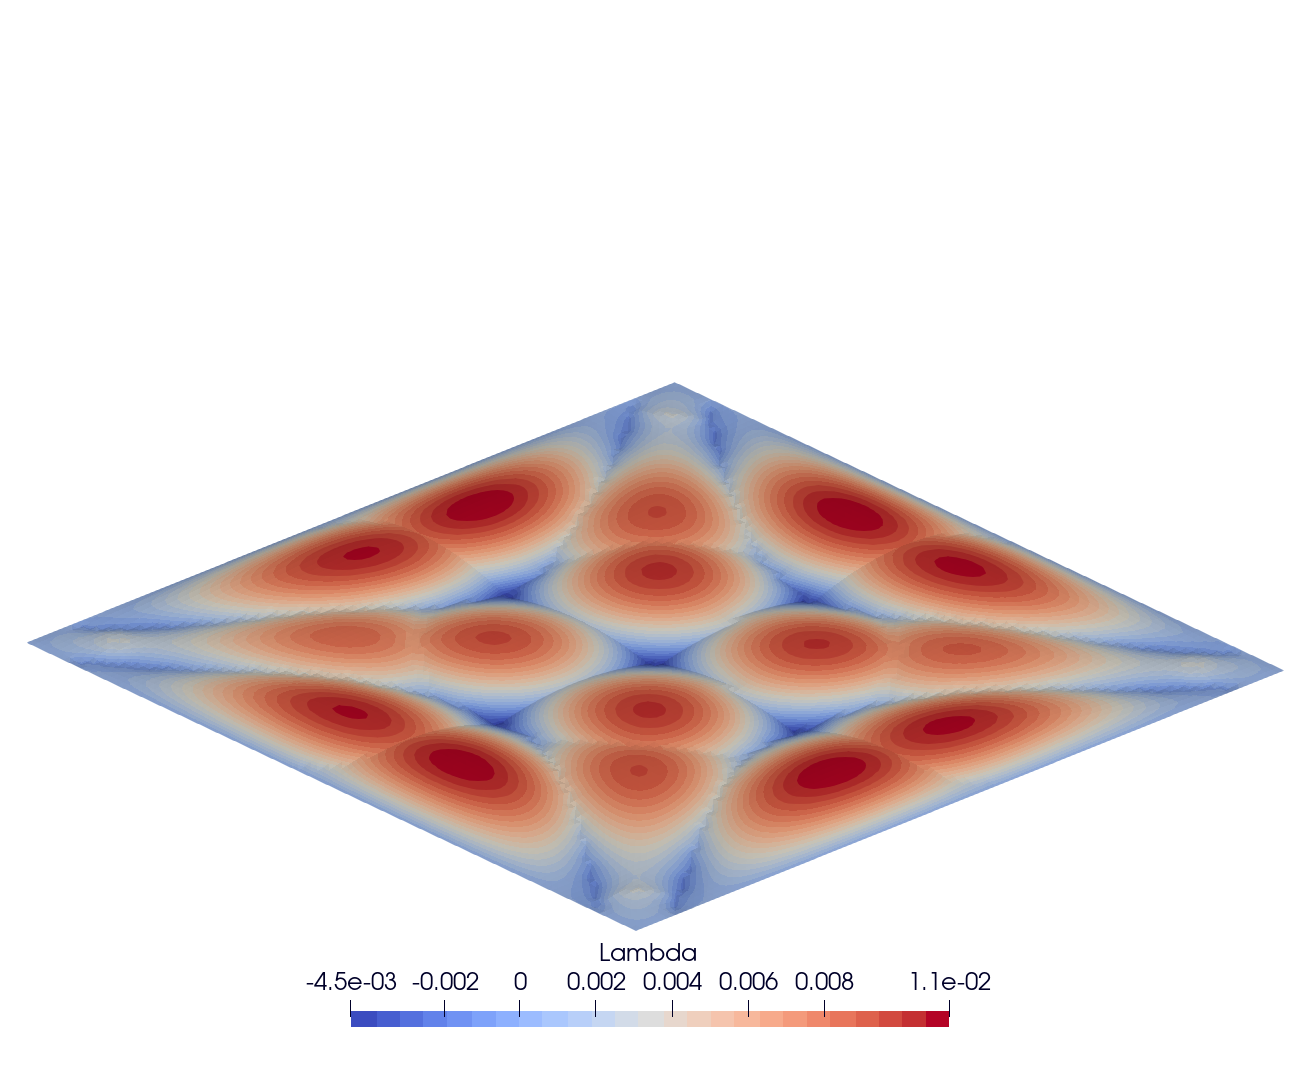
\includegraphics[width = 1.0\linewidth]{Figuras/Sensibilidade_amostras/lambda_wrapesc_NxNy101_Nsample4_4.png}
		\caption{$\text{N}_{x}^{\text{amostras}} = \text{N}_{y}^{\text{amostras}} = 4$.}
		\label{fig:lambda_wrapesc_NxNy101_Nsample4_4}
	\end{subfigure}
	\label{fig:lambda_sample_low_values}
\end{figure}

\begin{figure}[!ht]
	\centering
	\caption{À esquerda, curvas de nível do campo escalar de multiplicadores de Lagrange considerando os números de pontos amostrais retratados nas figuras \ref{fig:Nxy_sample_8_8} e \ref{fig:Nxy_sample_16_16}. À direita, as respectivas representações tridimensionais.}
	\begin{subfigure}[b]{0.45\linewidth}
		\centering
		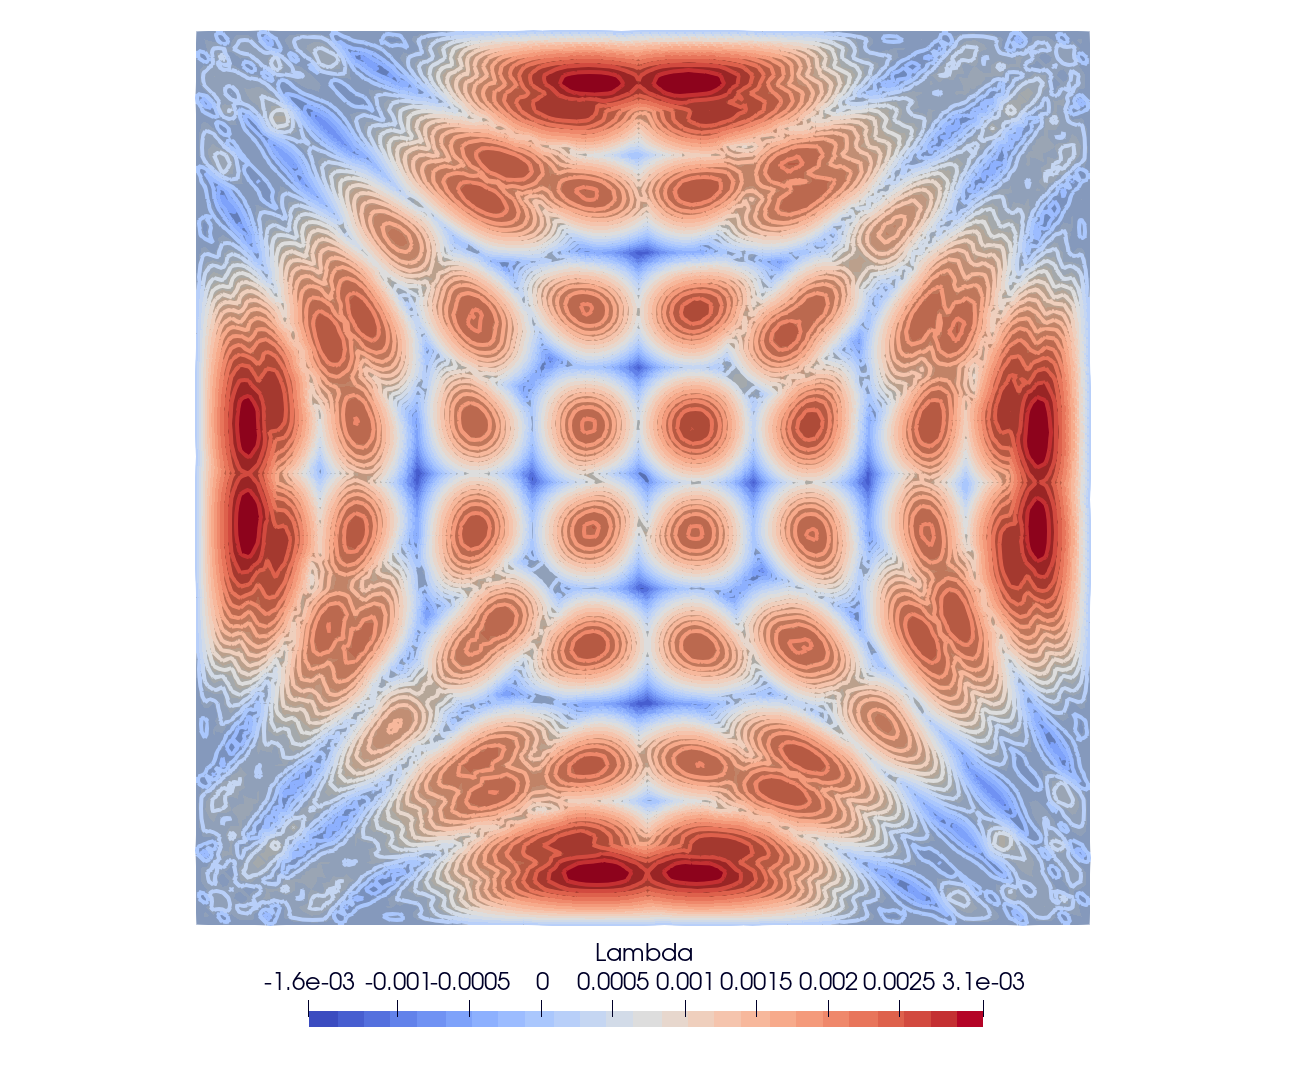
\includegraphics[width = 1.0\linewidth]{Figuras/Sensibilidade_amostras/lambda_contour_NxNy101_Nsample8_8.png}
		\caption{$\text{N}_{x}^{\text{amostras}} = \text{N}_{y}^{\text{amostras}} = 8$.}
		\label{fig:lambda_contour_NxNy101_Nsample8_8}
	\end{subfigure}
	\hfill
	\begin{subfigure}[b]{0.45\linewidth}
		\centering
		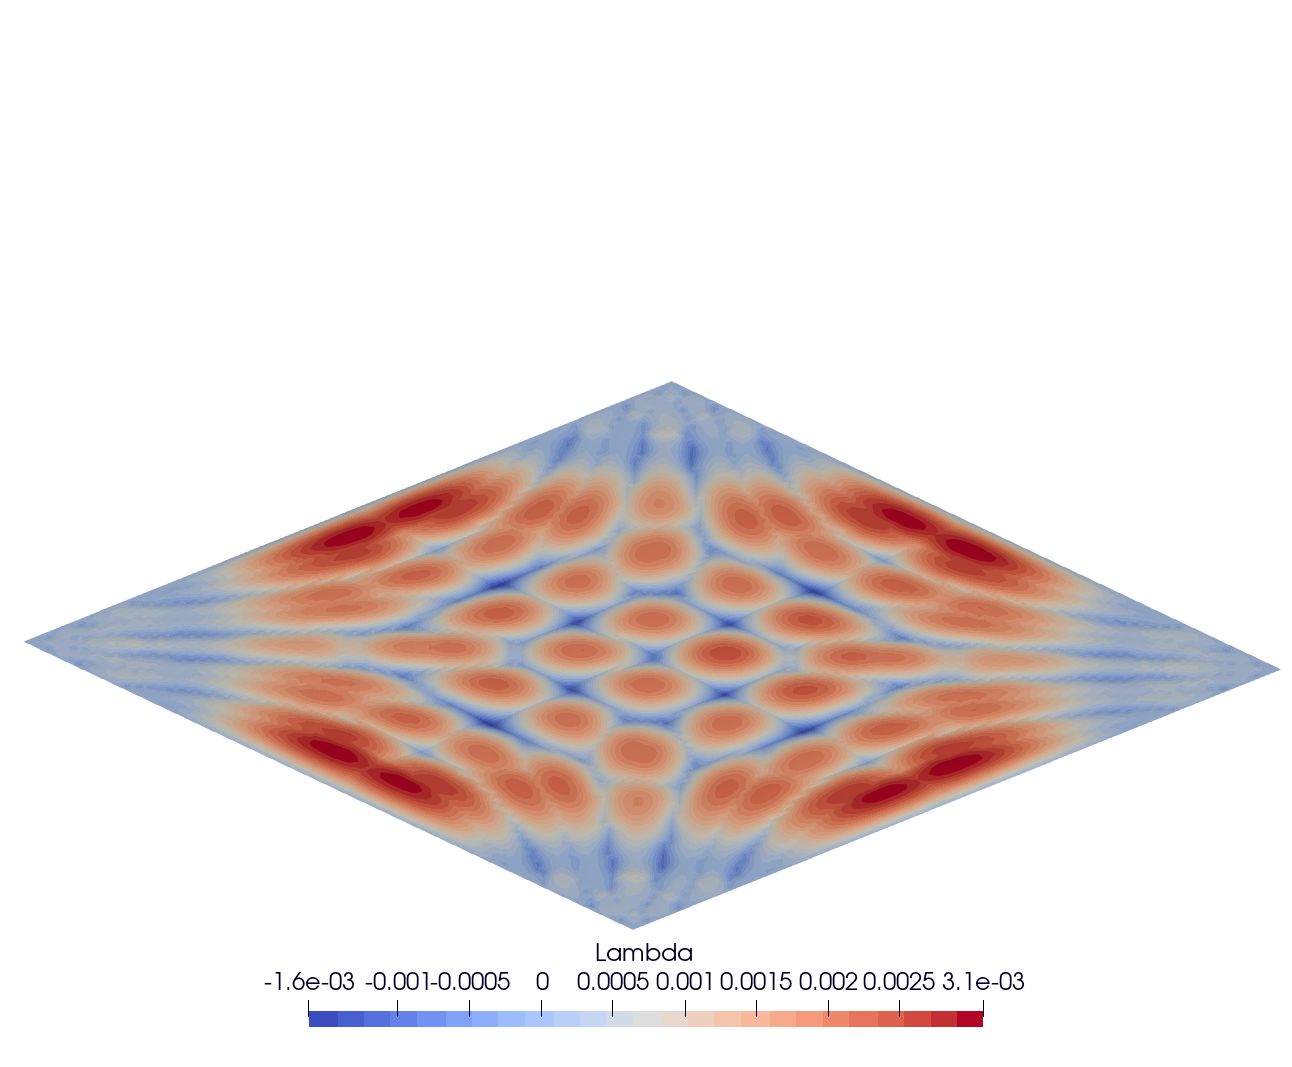
\includegraphics[width = 1.0\linewidth]{Figuras/Sensibilidade_amostras/lambda_wrapesc_NxNy101_Nsample8_8.png}
		\caption{$\text{N}_{x}^{\text{amostras}} = \text{N}_{y}^{\text{amostras}} = 8$.}
		\label{fig:lambda_wrapesc_NxNy101_Nsample8_8}
	\end{subfigure}
	\hfill
	\begin{subfigure}[b]{0.45\linewidth}
		\centering
		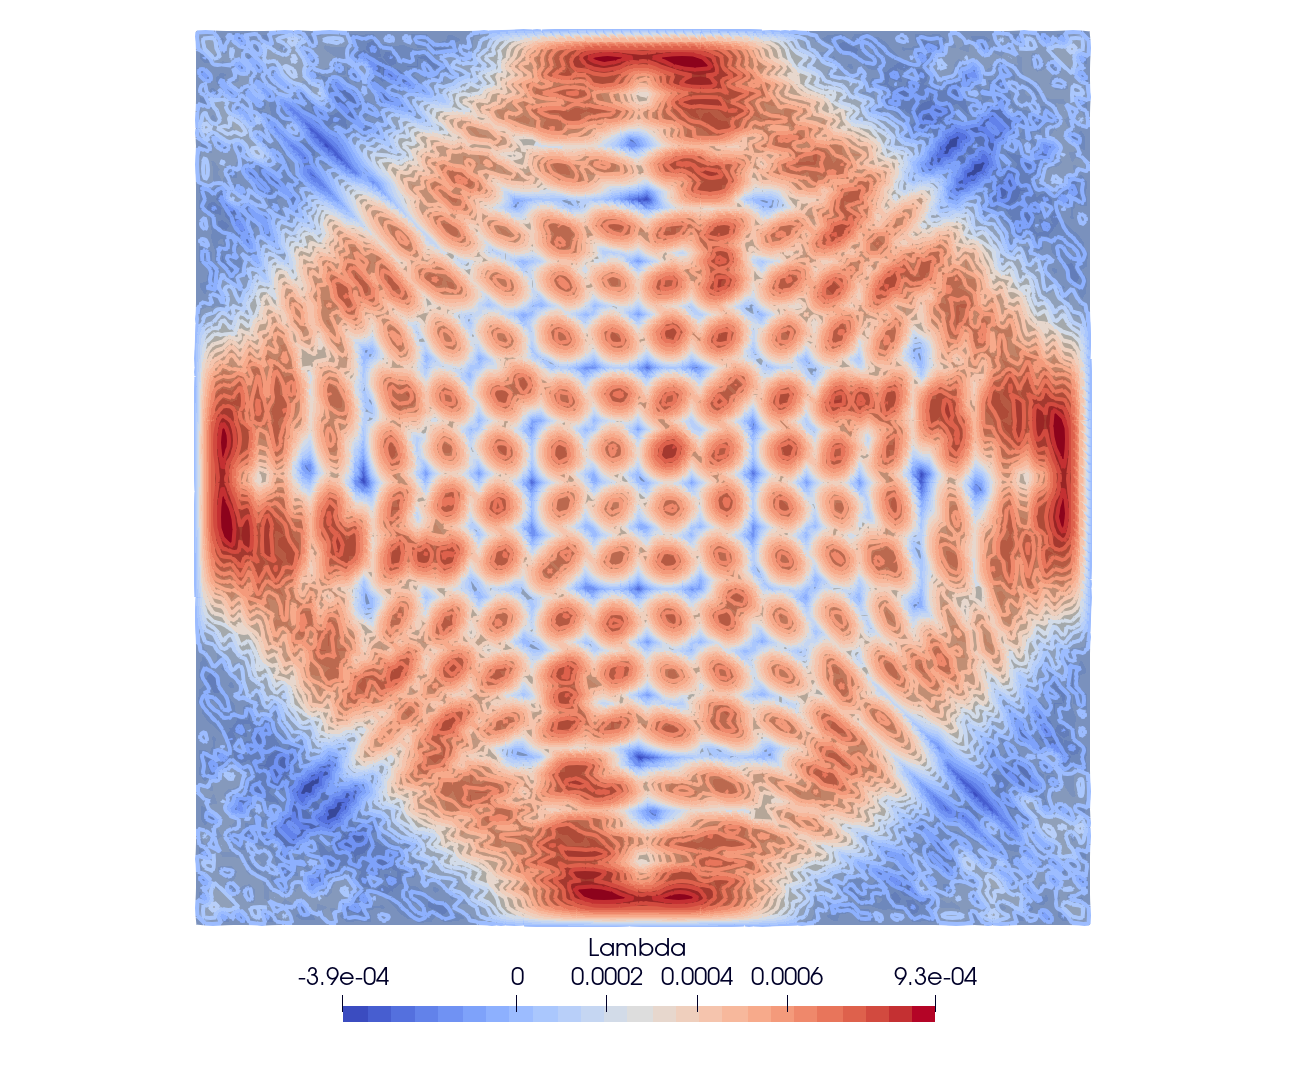
\includegraphics[width = 1.0\linewidth]{Figuras/Sensibilidade_amostras/lambda_contour_NxNy101_Nsample16_16.png}
		\caption{$\text{N}_{x}^{\text{amostras}} = \text{N}_{y}^{\text{amostras}} = 16$.}
		\label{fig:lambda_contour_NxNy101_Nsample16_16}
	\end{subfigure}
	\hfill
	\begin{subfigure}[b]{0.45\linewidth}
		\centering
		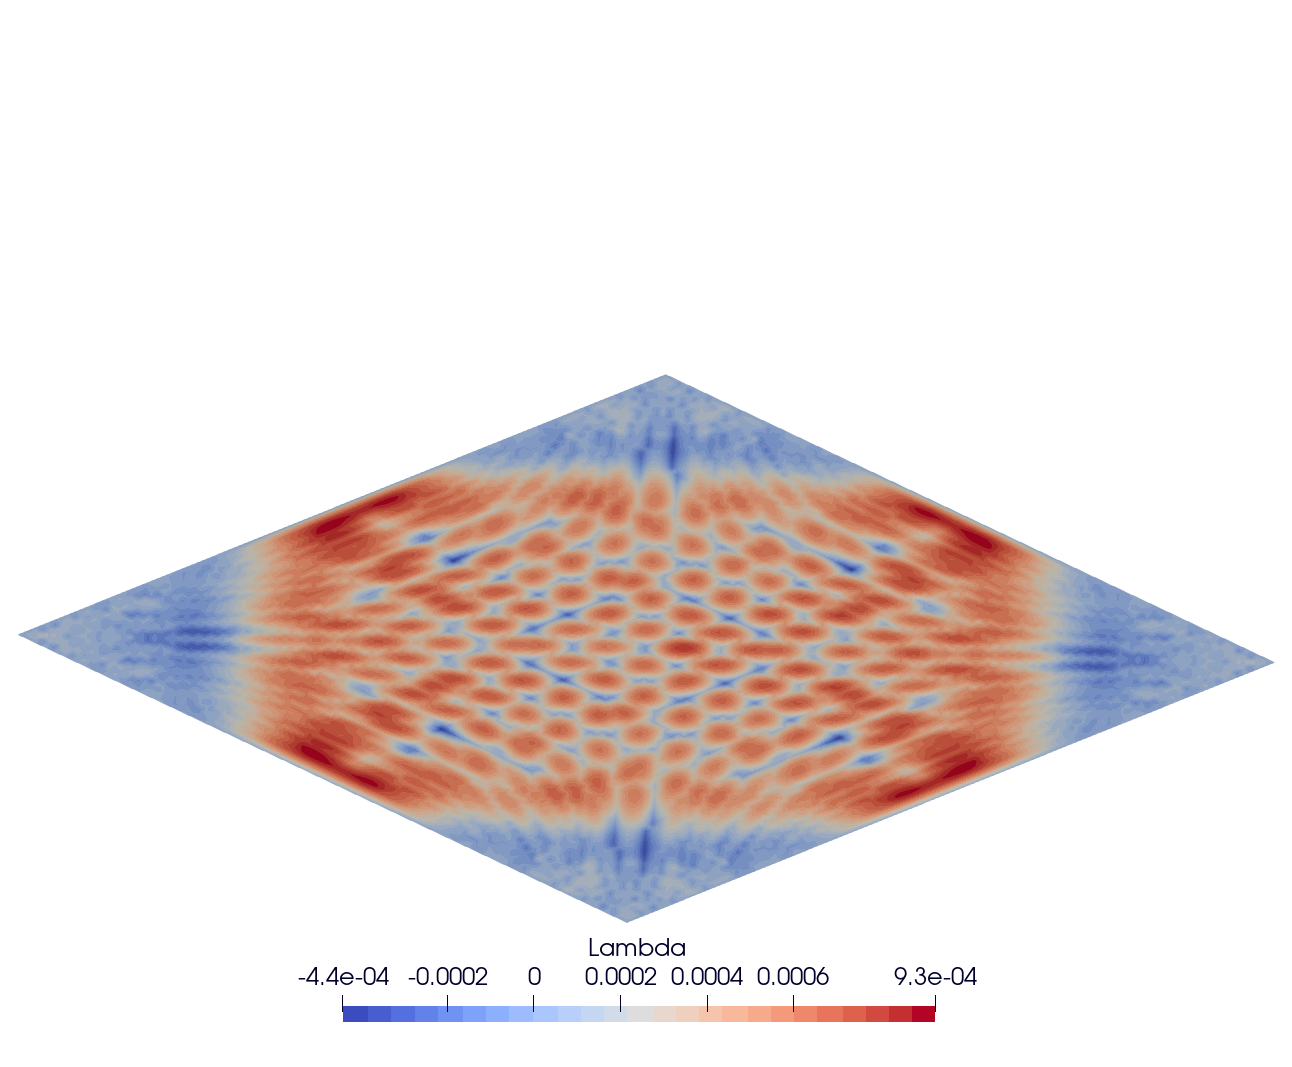
\includegraphics[width = 1.0\linewidth]{Figuras/Sensibilidade_amostras/lambda_wrapesc_NxNy101_Nsample16_16.png}
		\caption{$\text{N}_{x}^{\text{amostras}} = \text{N}_{y}^{\text{amostras}} = 16$.}
		\label{fig:lambda_wrapesc_NxNy101_Nsample16_16}
	\end{subfigure}
	\label{fig:lambda_sample_high_values}
\end{figure}

%Flux%
\begin{figure}[!ht]
	\centering
	\caption{$\mathbf{u}$, para os diferentes conjuntos de pontos amostrais, $(\text{N}_{x}^{\text{amostras}},\text{N}_{y}^{\text{amostras}})$, definidos na figura \ref{fig:Nxy_sample}.}
	\begin{subfigure}[b]{0.45\linewidth}
		\centering
		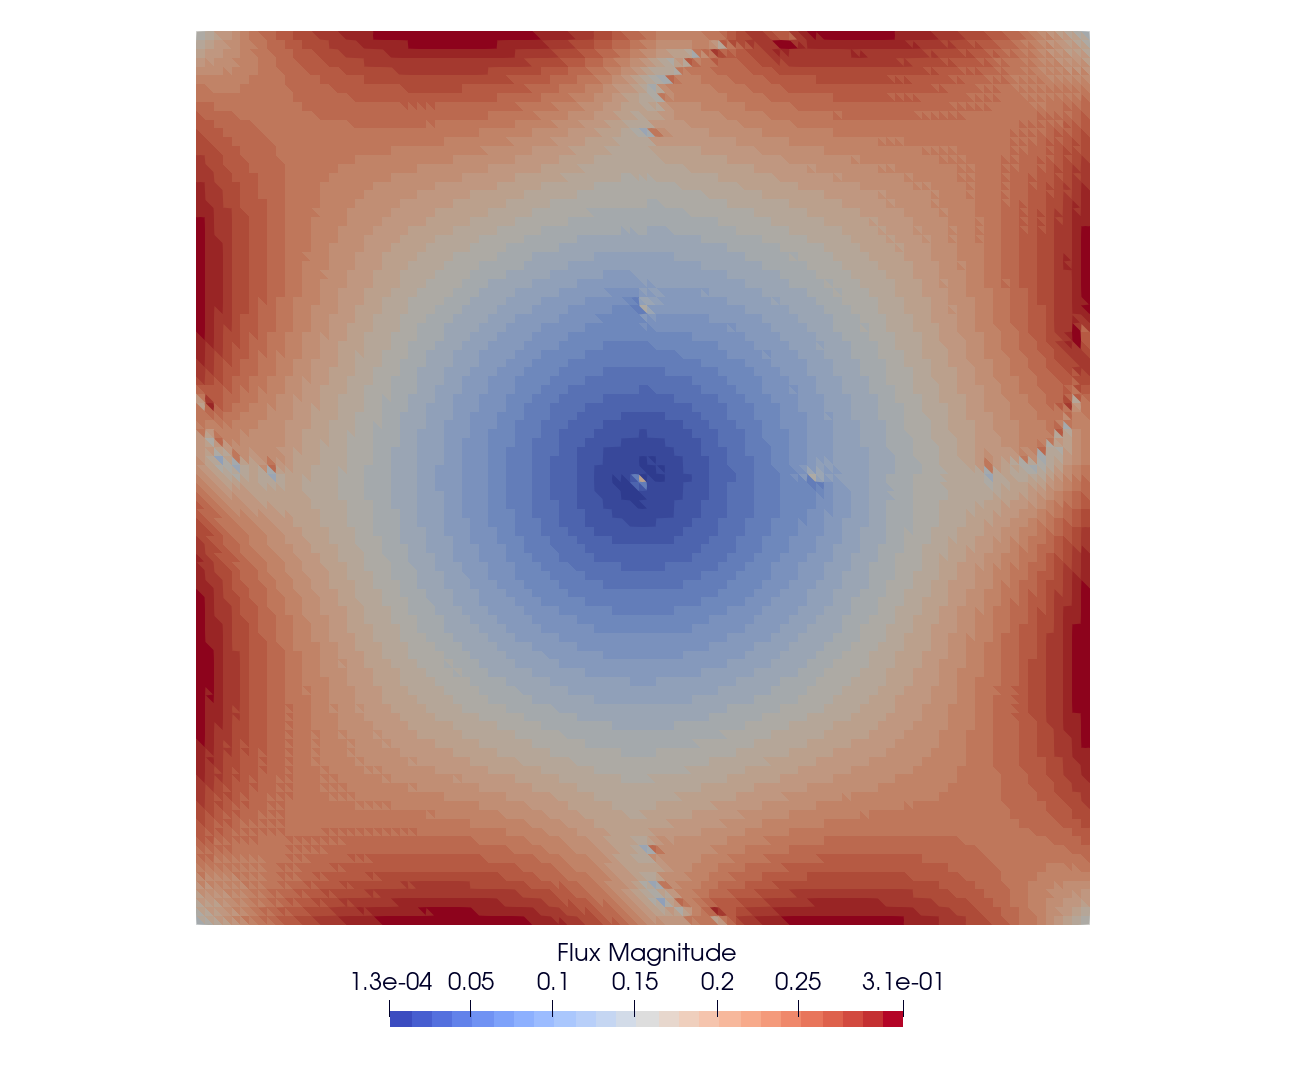
\includegraphics[width = 1.0\linewidth]{Figuras/Sensibilidade_amostras/flux_NxNy101_Nsample2_2.png}
		\caption{$\text{N}_{x}^{\text{amostras}} = \text{N}_{y}^{\text{amostras}} = 2$.}
		\label{fig:flux_NxNy101_Nsample2_2}
	\end{subfigure}
	\hfill
	\begin{subfigure}[b]{0.45\linewidth}
		\centering
		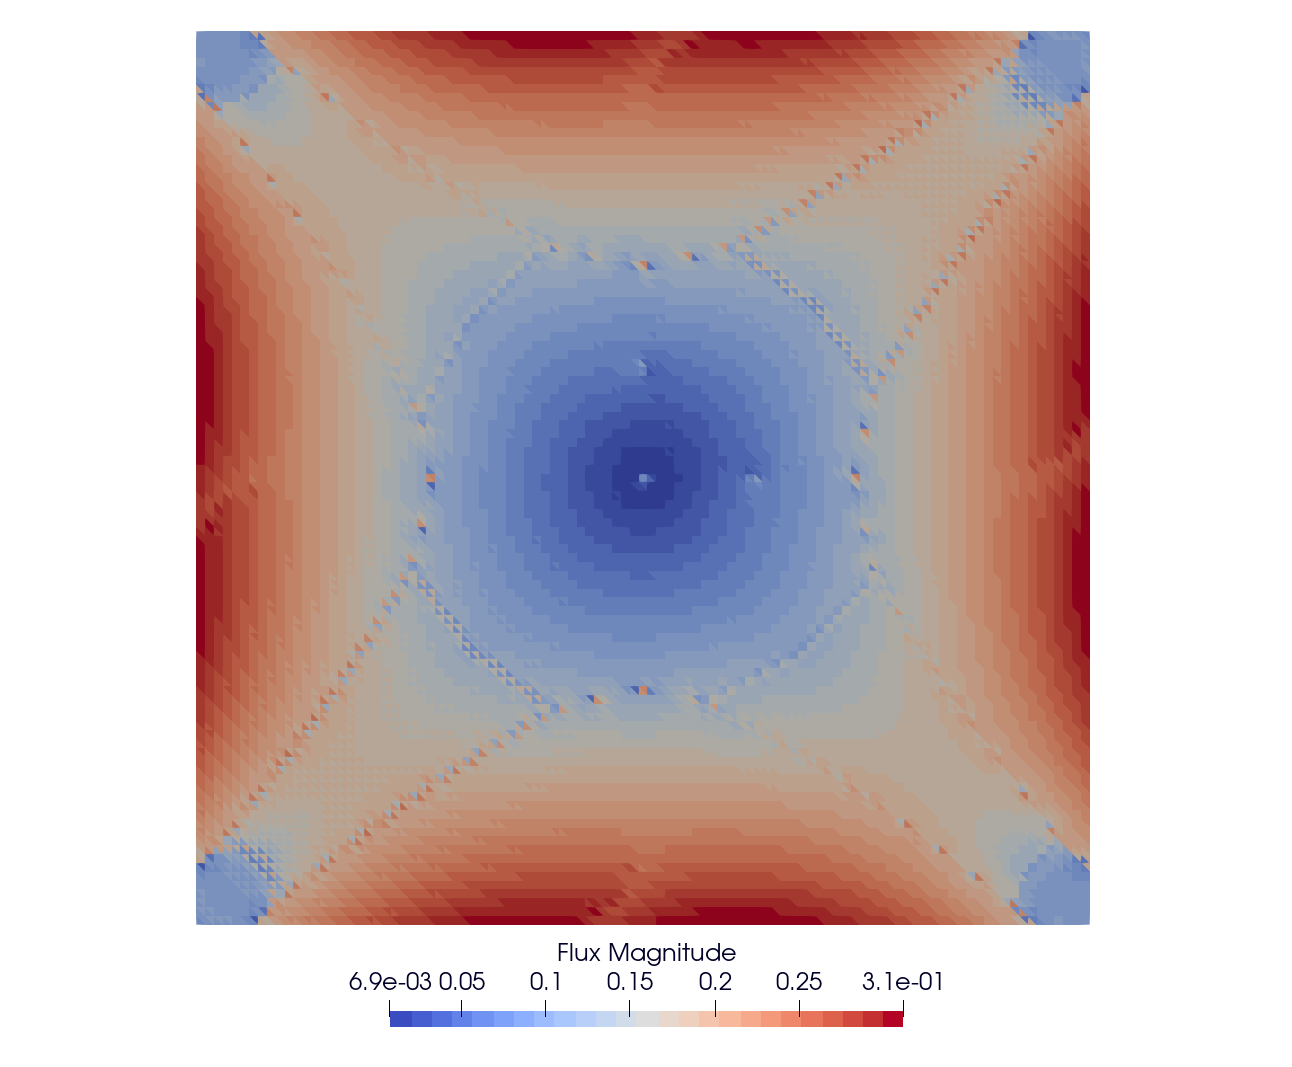
\includegraphics[width = 1.0\linewidth]{Figuras/Sensibilidade_amostras/flux_NxNy101_Nsample4_4.png}
		\caption{$\text{N}_{x}^{\text{amostras}} = \text{N}_{y}^{\text{amostras}} = 4$.}
		\label{fig:flux_NxNy101_Nsample4_4}
	\end{subfigure}
	\hfill
	\begin{subfigure}[b]{0.45\linewidth}
		\centering
		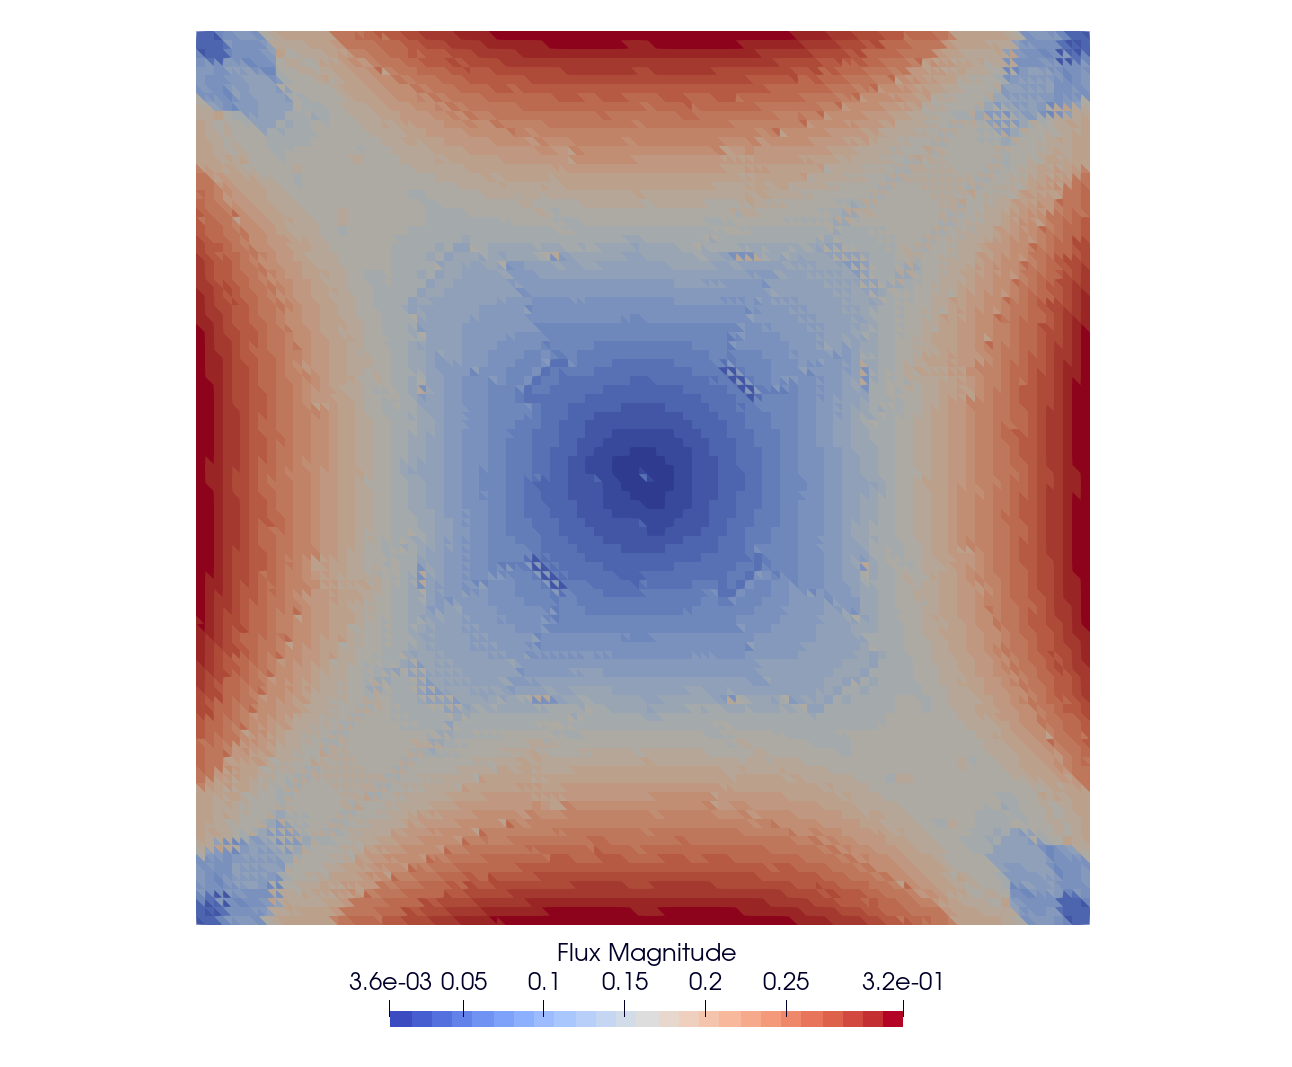
\includegraphics[width = 1.0\linewidth]{Figuras/Sensibilidade_amostras/flux_NxNy101_Nsample8_8.png}
		\caption{$\text{N}_{x}^{\text{amostras}} = \text{N}_{y}^{\text{amostras}} = 8$.}
		\label{fig:flux_NxNy101_Nsample8_8}
	\end{subfigure}
	\hfill
	\begin{subfigure}[b]{0.45\linewidth}
		\centering
		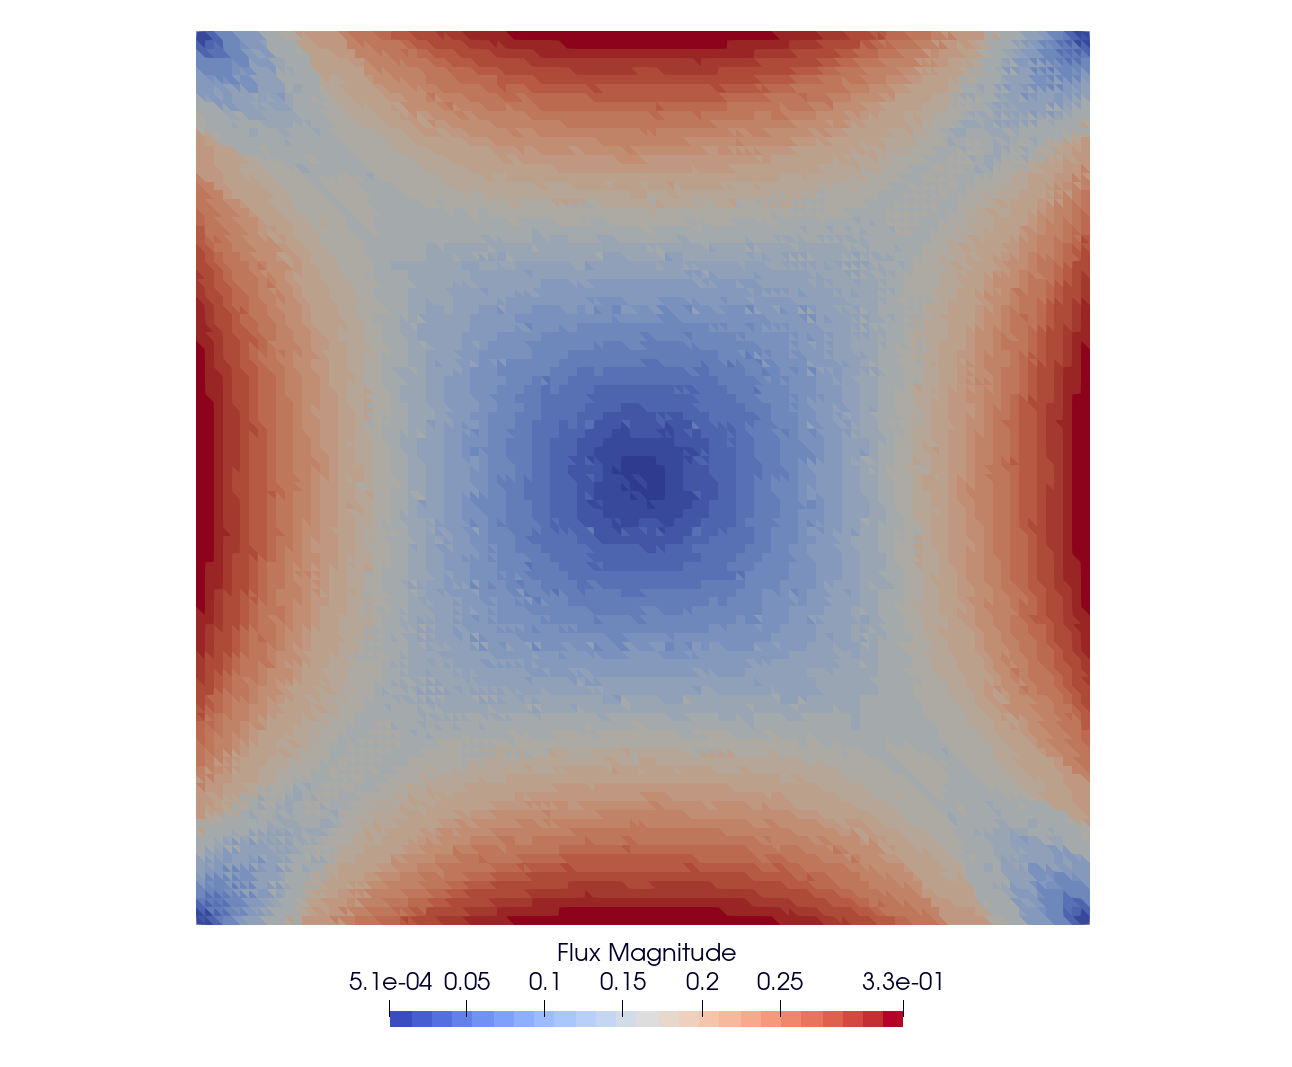
\includegraphics[width = 1.0\linewidth]{Figuras/Sensibilidade_amostras/flux_NxNy101_Nsample16_16.png}
		\caption{$\text{N}_{x}^{\text{amostras}} = \text{N}_{y}^{\text{amostras}} = 16$.}
		\label{fig:flux_NxNy101_Nsample16_16}
	\end{subfigure}
	\label{fig:flux_NxNy101_Nsample}
\end{figure}

%mu%
\begin{figure}[!ht]
	\centering
	\caption{$\boldsymbol{\mu}$ para os diferentes conjuntos de pontos amostrais $(\text{N}_{x}^{\text{amostras}},\text{N}_{y}^{\text{amostras}})$, definidos na figura \ref{fig:Nxy_sample}.}
	\begin{subfigure}[b]{0.45\linewidth}
		\centering
		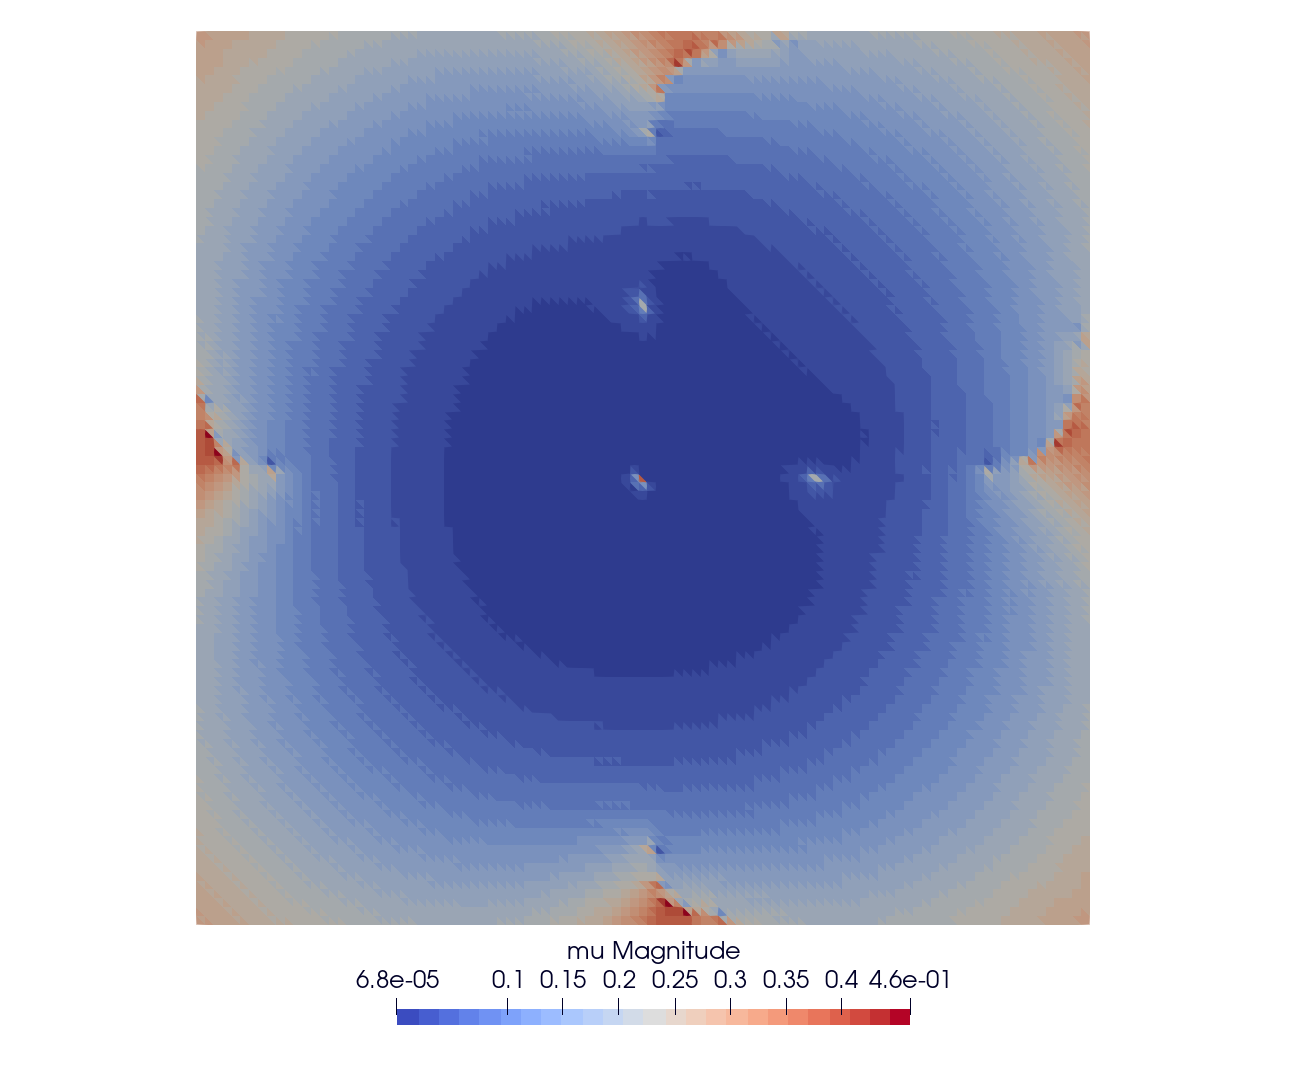
\includegraphics[width = 1.0\linewidth]{Figuras/Sensibilidade_amostras/mu_NxNy101_Nsample2_2.png}
		\caption{$\text{N}_{x}^{\text{amostras}} = \text{N}_{y}^{\text{amostras}} = 2$.}
		\label{fig:mu_NxNy101_Nsample2_2}
	\end{subfigure}
	\hfill
	\begin{subfigure}[b]{0.45\linewidth}
		\centering
		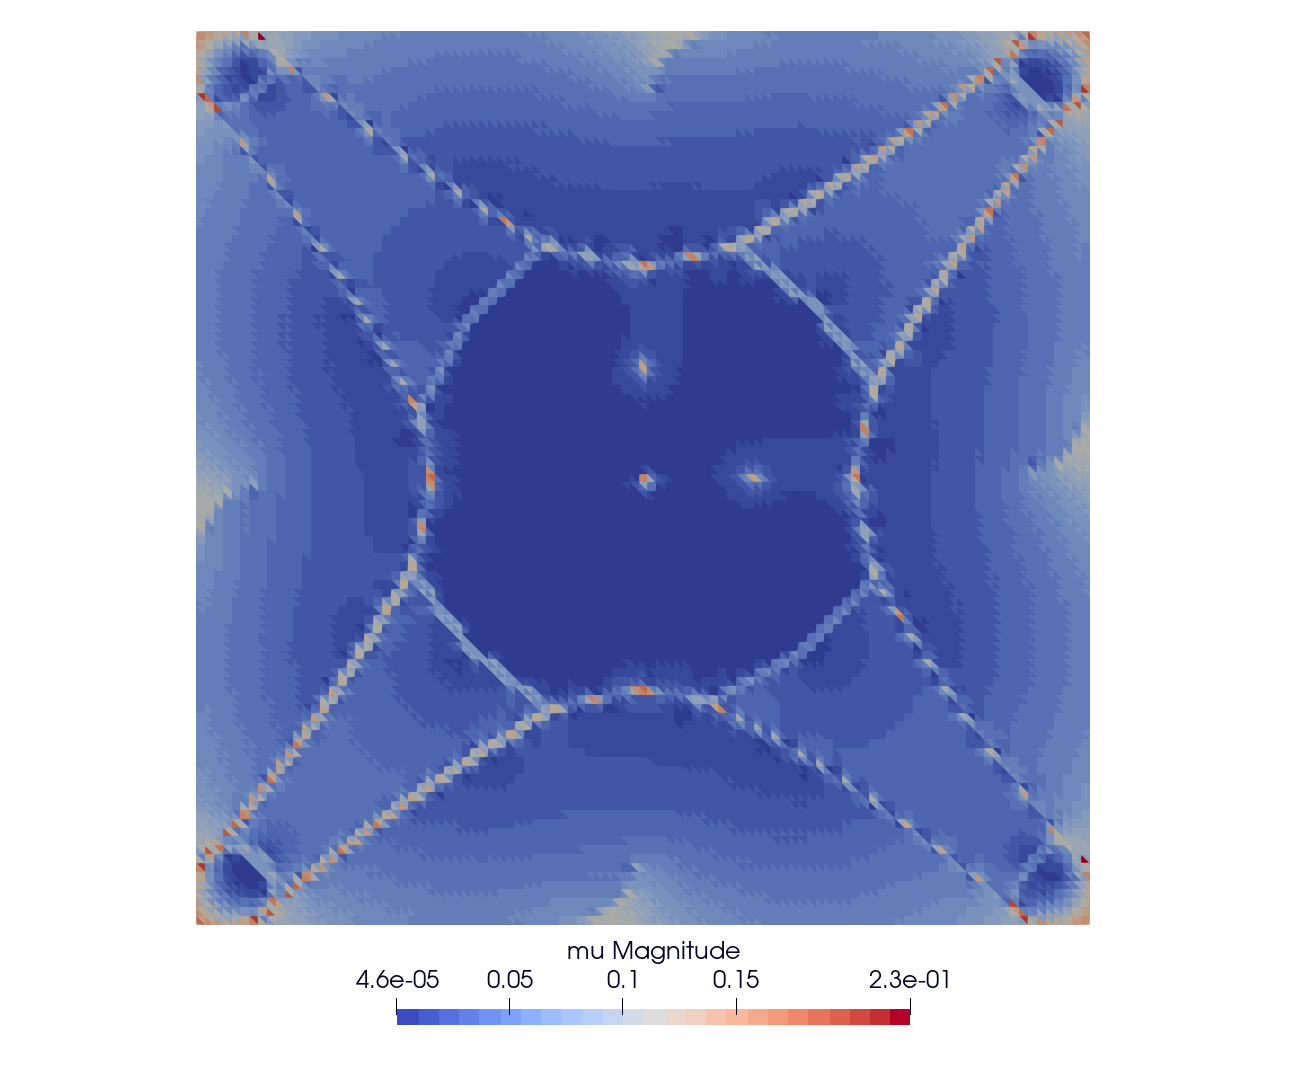
\includegraphics[width = 1.0\linewidth]{Figuras/Sensibilidade_amostras/mu_NxNy101_Nsample4_4.png}
		\caption{$\text{N}_{x}^{\text{amostras}} = \text{N}_{y}^{\text{amostras}} = 4$.}
		\label{fig:mu_NxNy101_Nsample4_4}
	\end{subfigure}
	\hfill
	\begin{subfigure}[b]{0.45\linewidth}
		\centering
		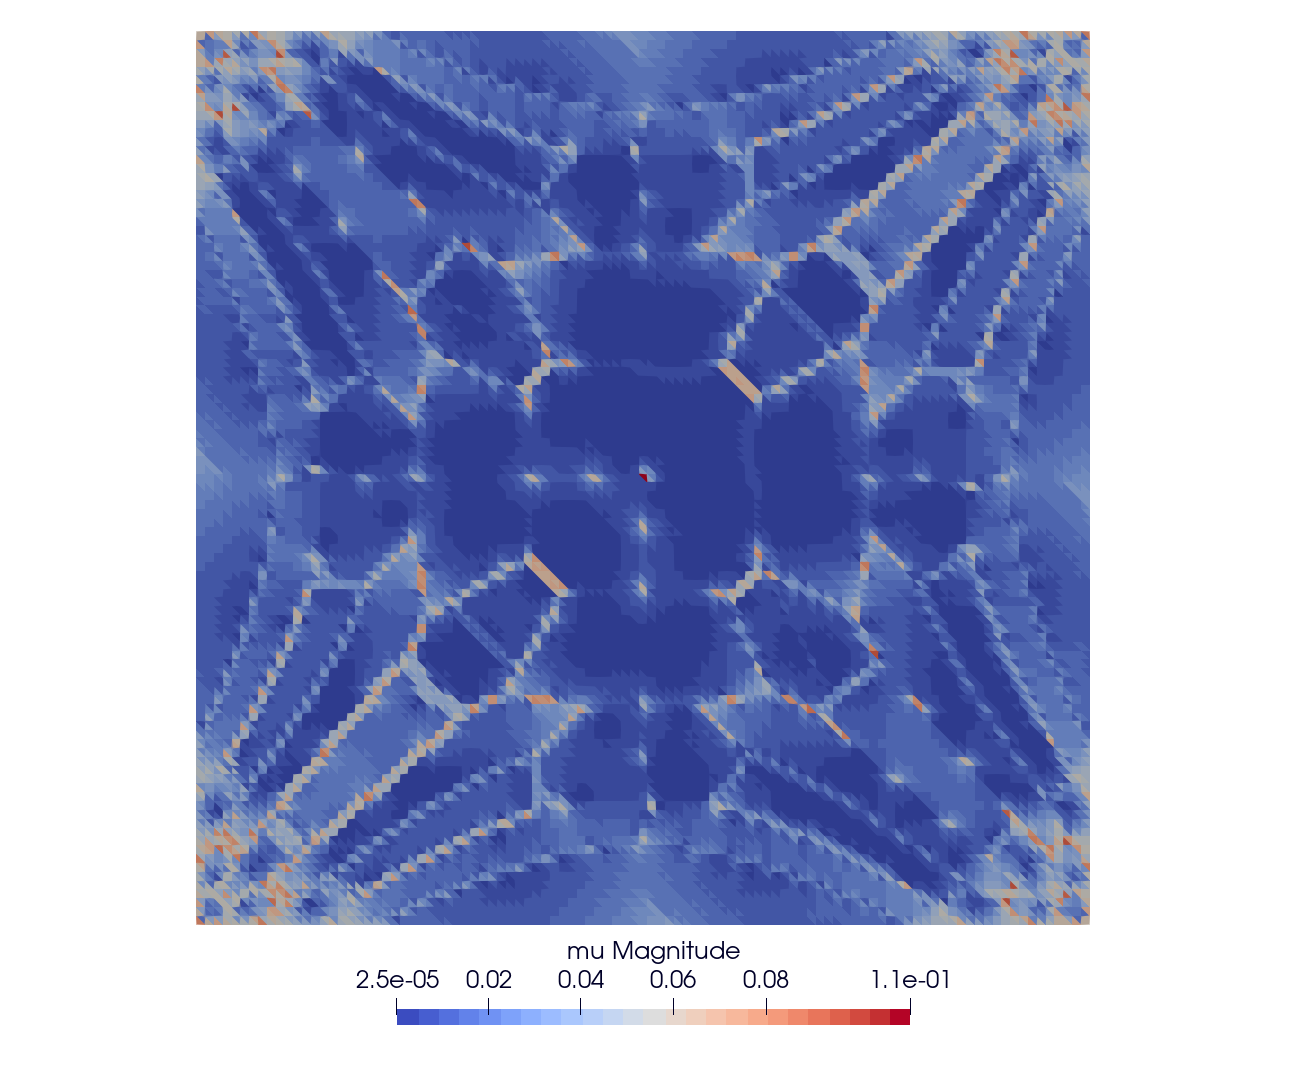
\includegraphics[width = 1.0\linewidth]{Figuras/Sensibilidade_amostras/mu_NxNy101_Nsample8_8.png}
		\caption{$\text{N}_{x}^{\text{amostras}} = \text{N}_{y}^{\text{amostras}} = 8$.}
		\label{fig:mu_NxNy101_Nsample8_8}
	\end{subfigure}
	\hfill
	\begin{subfigure}[b]{0.45\linewidth}
		\centering
		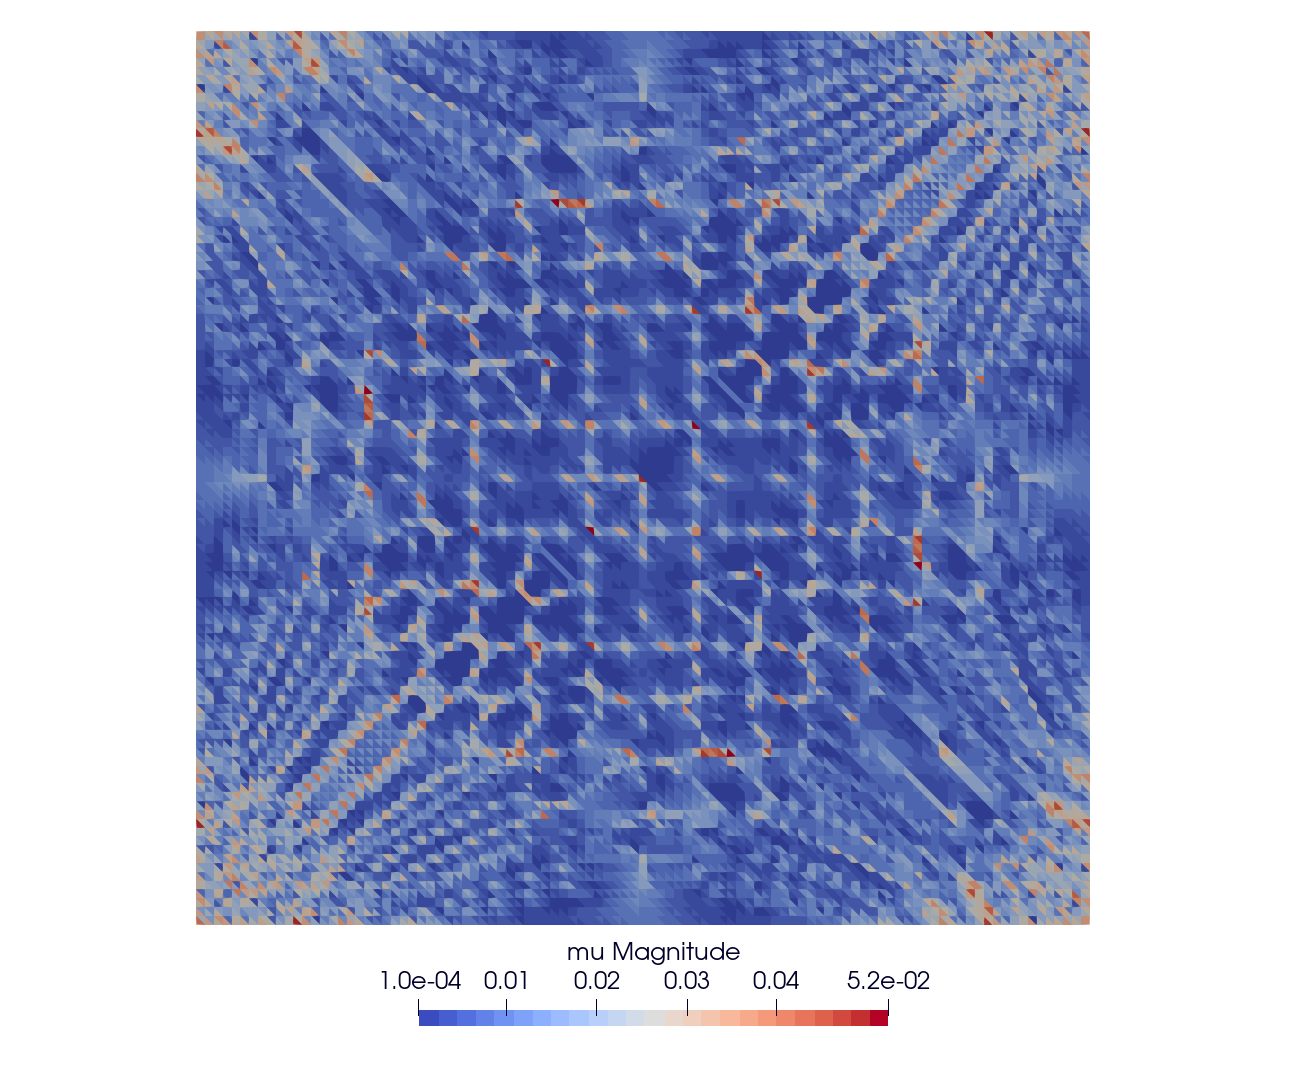
\includegraphics[width = 1.0\linewidth]{Figuras/Sensibilidade_amostras/mu_NxNy101_Nsample16_16.png}
		\caption{$\text{N}_{x}^{\text{amostras}} = \text{N}_{y}^{\text{amostras}} = 16$.}
		\label{fig:mu_NxNy101_Nsample16_16}
	\end{subfigure}
	\label{fig:mu_NxNy101_Nsample}
\end{figure}




\clearpage
\subsection{Sensibilidade quanto a discretização da malha de elementos finitos}

Neste estudo de caso, fixou-se o número de pontos amostrais em cada uma das direções coordenadas, em particular, admitiu-se $\text{N}_{x}^{\text{amostras}} = \text{N}_{y}^{\text{amostras}} = 4$ e avaliou-se o comportamento de $p$, $\lambda$, $\mathbf{u}$ e $\boldsymbol{\mu}$ sobre diferentes discretizações da malha de elementos finitos. Nesse sentido, foram empregadas quatro distintas discretizações: $25 \times 25$, $50 \times 50$, $100 \times 100$ e $200 \times 200$ 
elementos. Os resultados obtido, então, são apresentados e discutidos a seguir.  


%Pressure%
\begin{figure}[!ht]
	\centering
	\caption{À esquerda, curvas de nível do campo escalar de pressões, $p$, considerando $\text{N}_{x}^{\text{amostras}} = \text{N}_{y}^{\text{amostras}} = 4$ e malhas de elementos finitos grosseiras. À direita, as respectivas representações tridimensionais.}
	\begin{subfigure}[b]{0.45\linewidth}
		\centering
		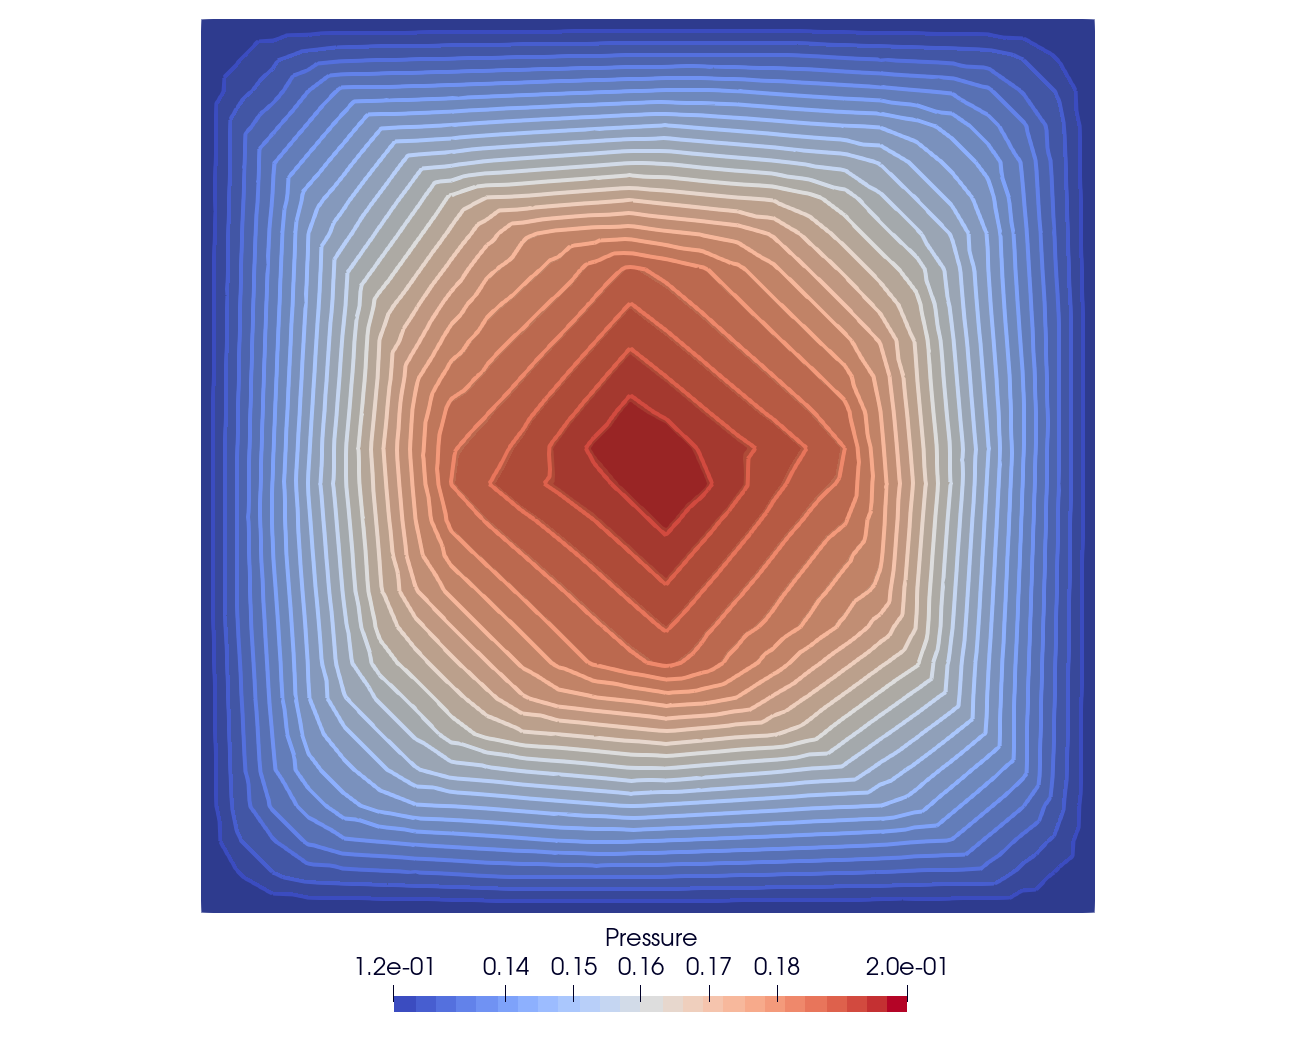
\includegraphics[width = 1.0\linewidth]{Figuras/Sensibilidade_malha_elemfin/pressure_contour_Nsample4_Nxy25.png}
		\caption{$\text{N}_{x} = \text{N}_{y} = 25$.}
		\label{fig:pressure_contour_Nsample4_Nxy25}
	\end{subfigure}
	\hfill
	\begin{subfigure}[b]{0.45\linewidth}
		\centering
		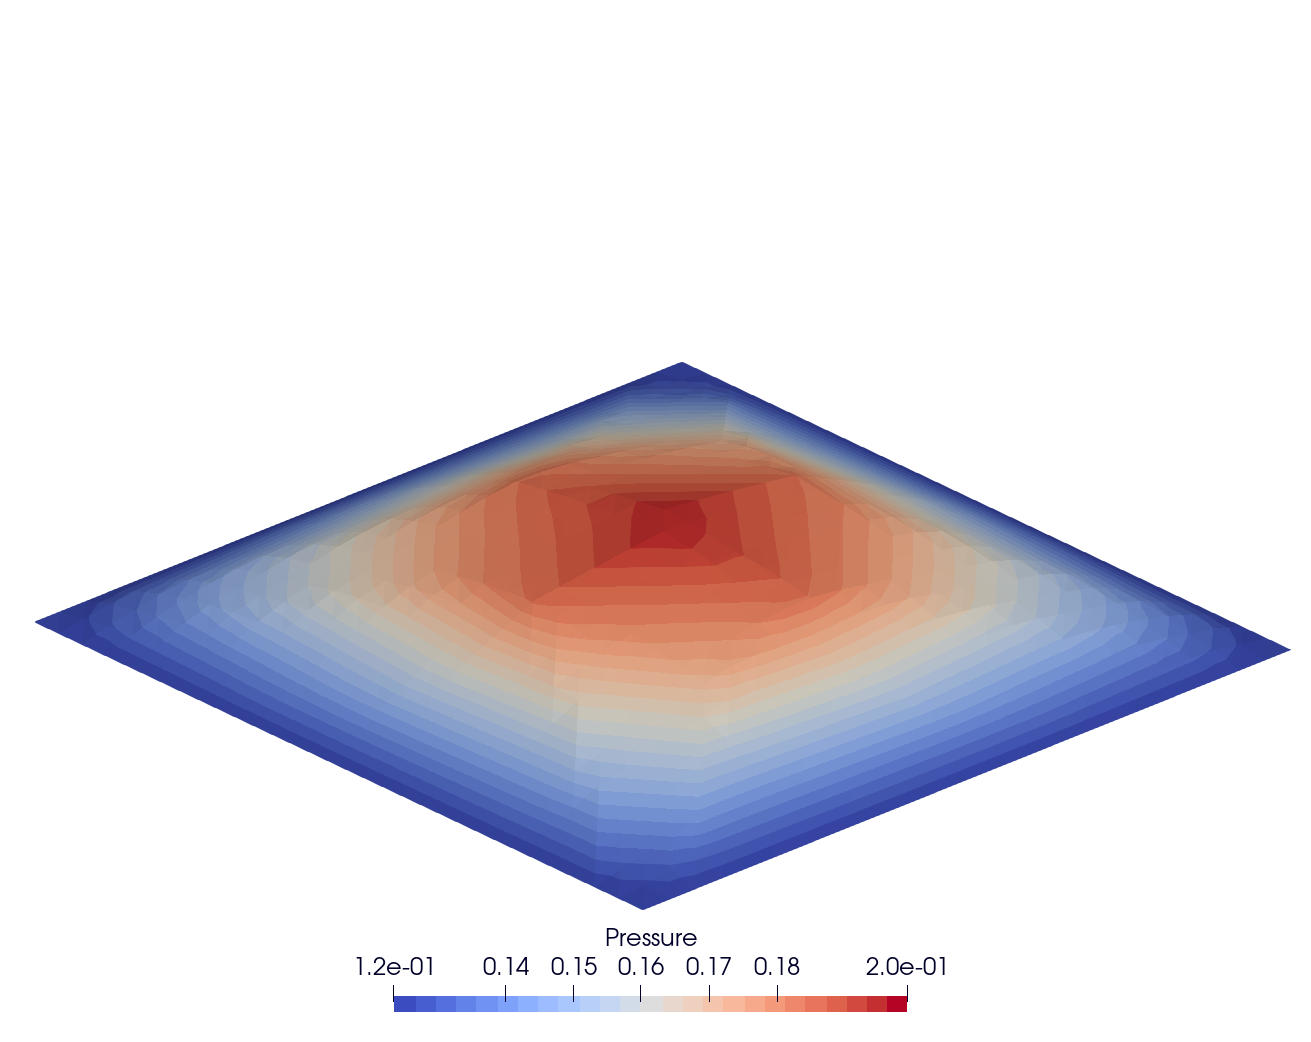
\includegraphics[width = 1.0\linewidth]{Figuras/Sensibilidade_malha_elemfin/pressure_wrapesc_Nsample4_Nxy25.png}
		\caption{$\text{N}_{x} = \text{N}_{y} = 25$.}
		\label{fig:pressure_wrapesc_Nsample4_Nxy25}
	\end{subfigure}
	\hfill
	\begin{subfigure}[b]{0.45\linewidth}
		\centering
		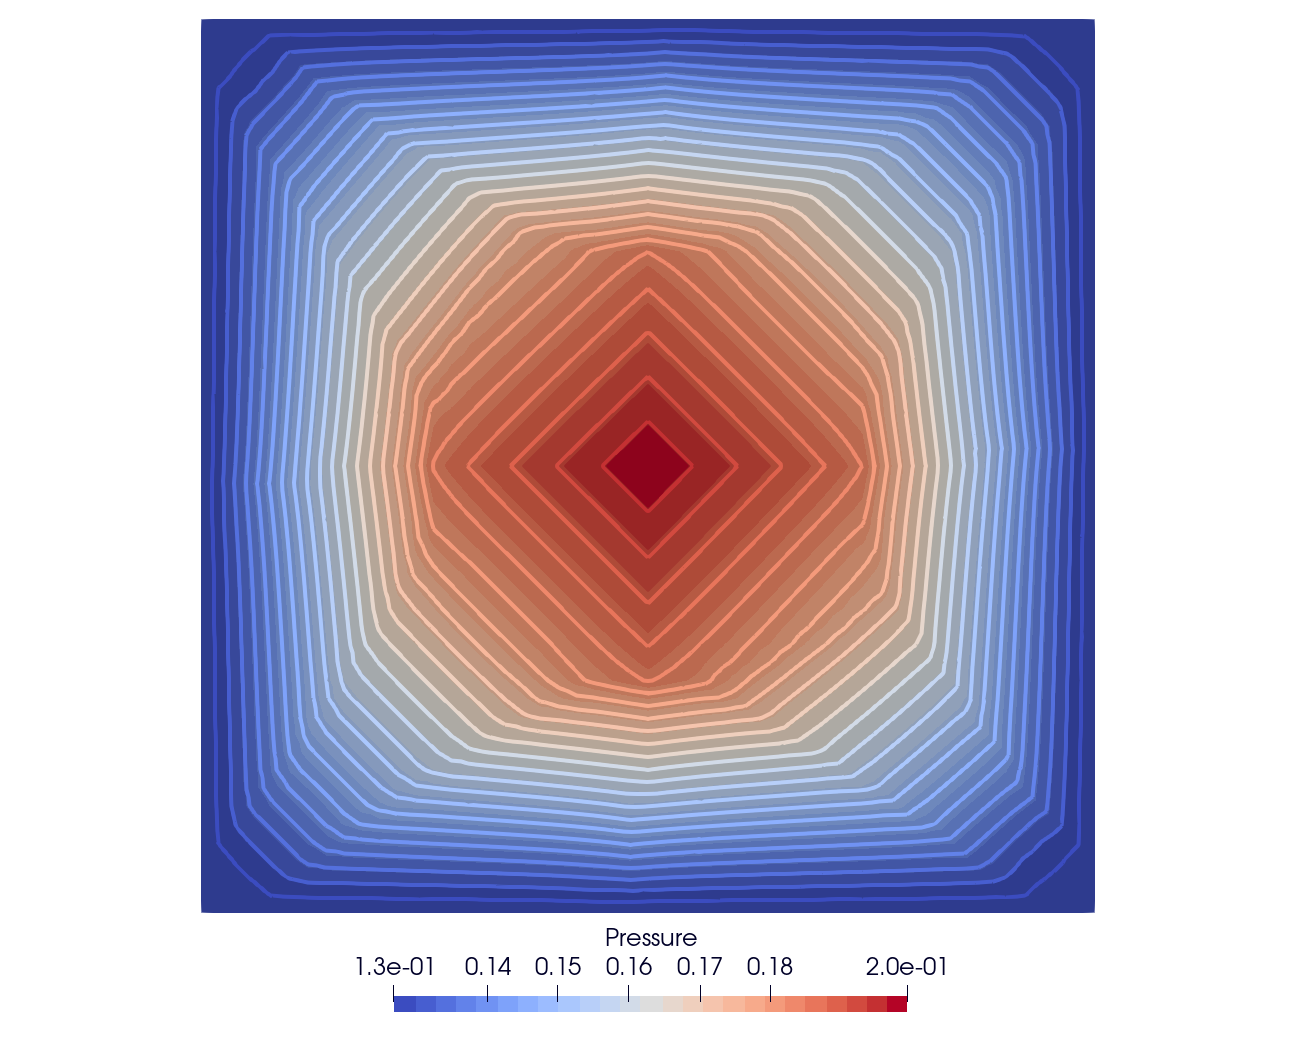
\includegraphics[width = 1.0\linewidth]{Figuras/Sensibilidade_malha_elemfin/pressure_contour_Nsample4_Nxy50.png}
		\caption{$\text{N}_{x} = \text{N}_{y} = 50$.}
		\label{fig:pressure_contour_Nsample4_Nxy50}
	\end{subfigure}
	\hfill
	\begin{subfigure}[b]{0.45\linewidth}
		\centering
		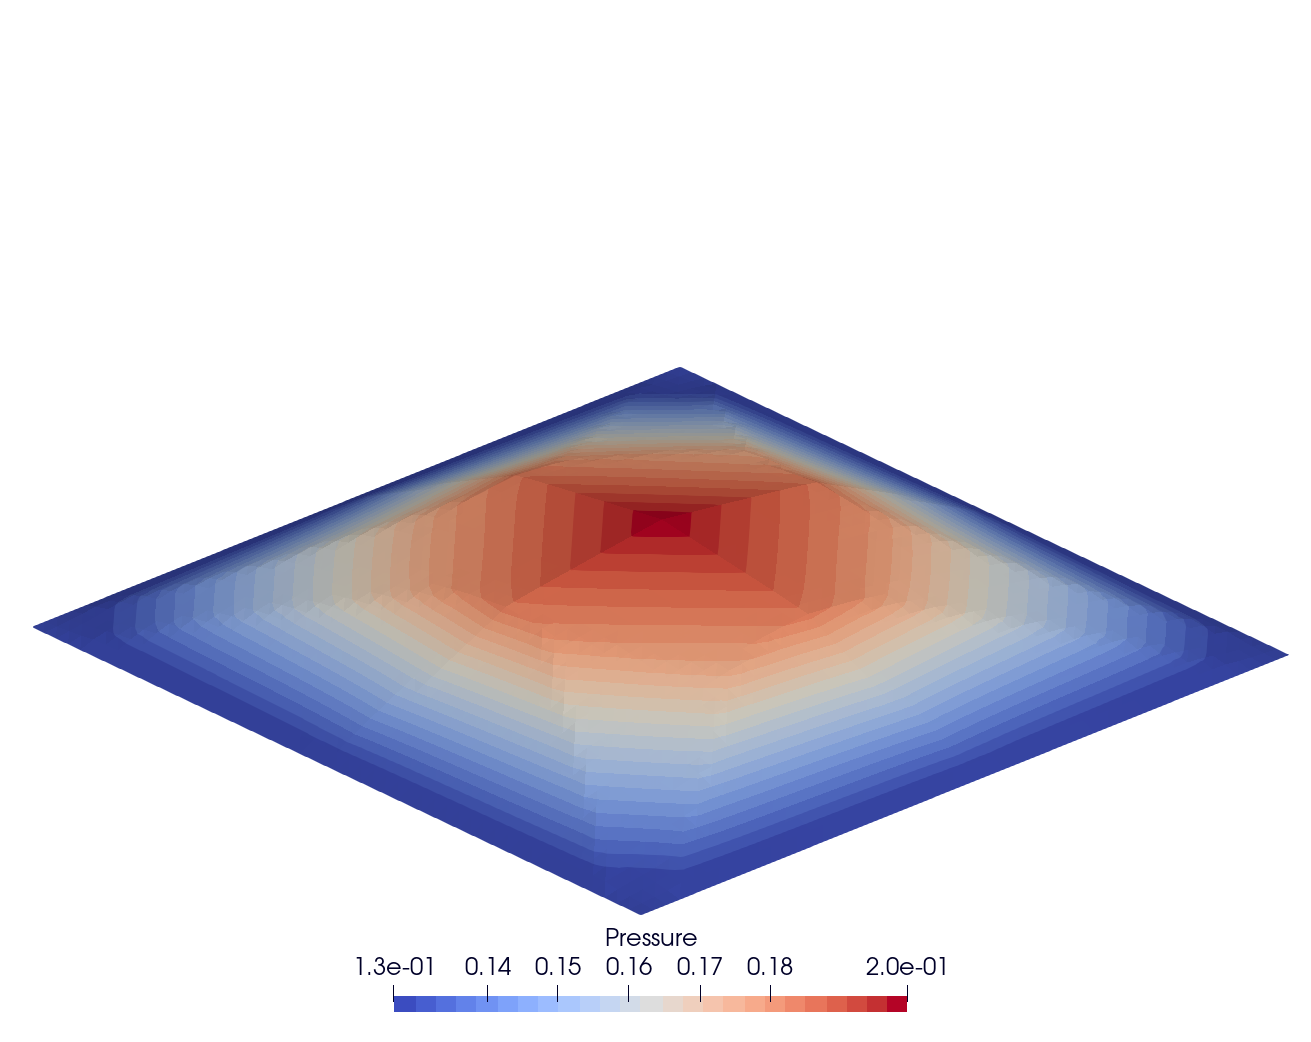
\includegraphics[width = 1.0\linewidth]{Figuras/Sensibilidade_malha_elemfin/pressure_wrapesc_Nsample4_Nxy50.png}
		\caption{$\text{N}_{x} = \text{N}_{y} = 50$.}
		\label{fig:pressure_wrapesc_Nsample4_Nxy50}
	\end{subfigure}
	\label{fig:pressure_mesh_coarse}
\end{figure}

Nas figuras \ref{fig:pressure_mesh_coarse} e \ref{fig:pressure_mesh_fine} são apresentados os os resultados do referido estudo para o campo escalar de pressões. De fato, a solução obtida assemelha-se àquela apresentada na figura \ref{fig:pressure_contour_NxNy101_Nsample4_4}, muito embora, com o aumento contínuo do número de elementos na malha, a solução torne-se gradualmente mais suave. Deve-se pontual, ademais, que as soluções, embora mais suaves, ainda distam daquela advinda da solução do problema de Poisson original -- \textit{i.e.} aquela que seria obtida quando:

\begin{equation}
	\lim_{(\mathcal{M},\mathcal{N})\rightarrow \infty}p(x,y) = p_{\text{\tiny{Poisson}}}(x,y), \quad 
	\begin{cases}
		\mathcal{M} = \text{N}_{x}^{\text{amostras}} \\
		\mathcal{N} = \text{N}_{y}^{\text{amostras}}
	\end{cases}.
\end{equation}

\begin{figure}[!ht]
	\centering
	\caption{À esquerda, curvas de nível do campo escalar de pressões, $p$, considerando $\text{N}_{x}^{\text{amostras}} = \text{N}_{y}^{\text{amostras}} = 4$ e malhas de elementos finitos refinadas. À direita, as respectivas representações tridimensionais.}
	\begin{subfigure}[b]{0.45\linewidth}
		\centering
		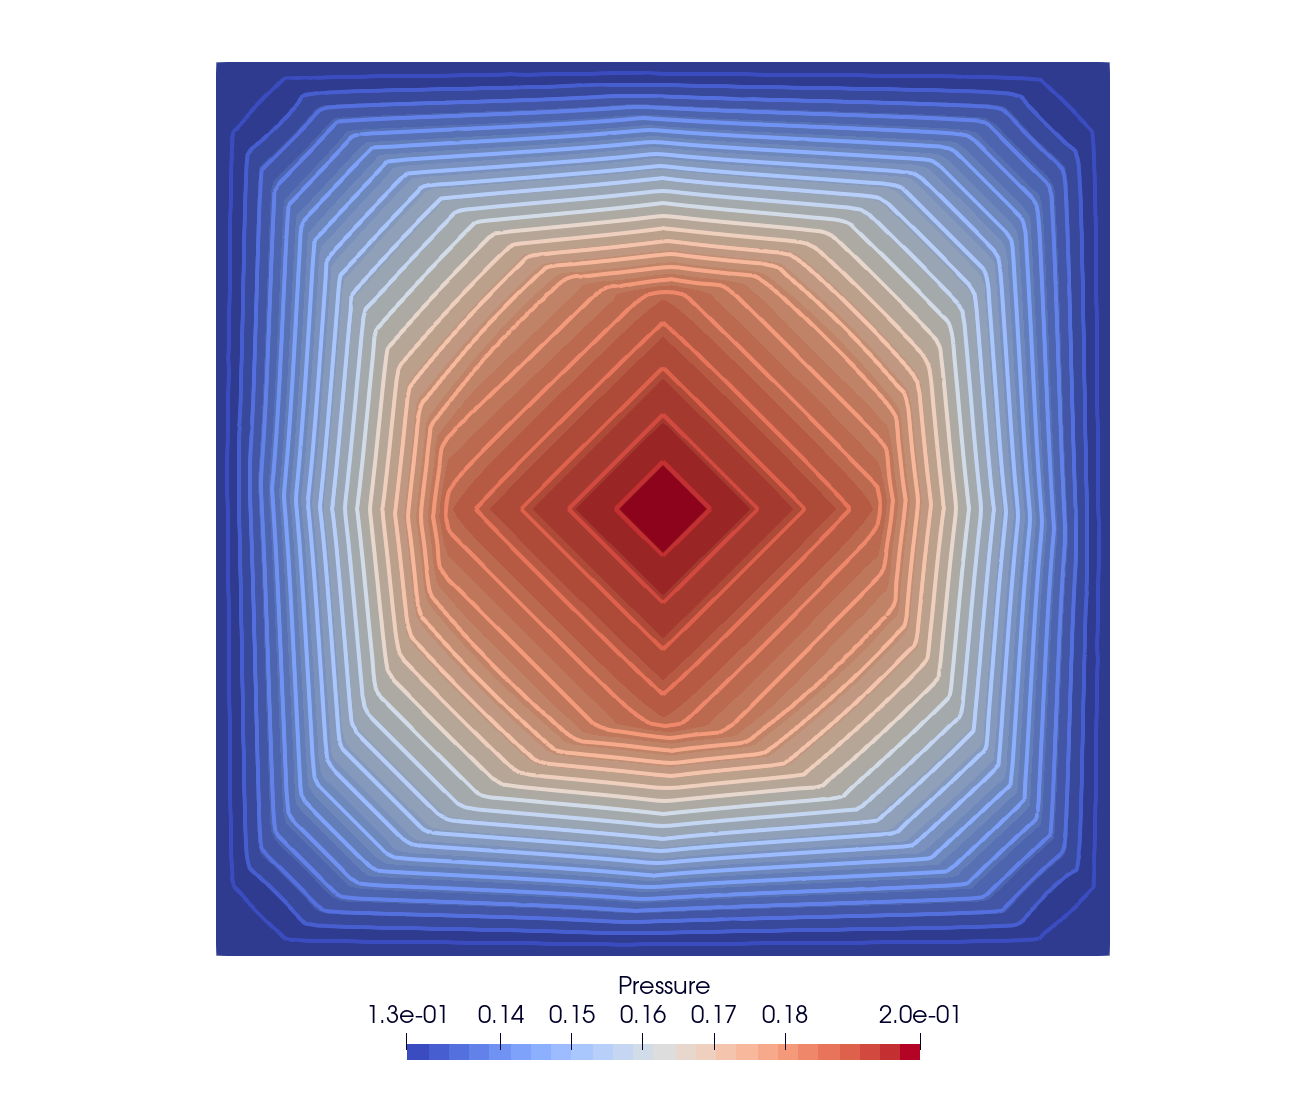
\includegraphics[width = 1.0\linewidth]{Figuras/Sensibilidade_malha_elemfin/pressure_contour_Nsample4_Nxy100.png}
		\caption{$\text{N}_{x} = \text{N}_{y} = 100$.}
		\label{fig:pressure_contour_Nsample4_Nxy100}
	\end{subfigure}
	\hfill
	\begin{subfigure}[b]{0.45\linewidth}
		\centering
		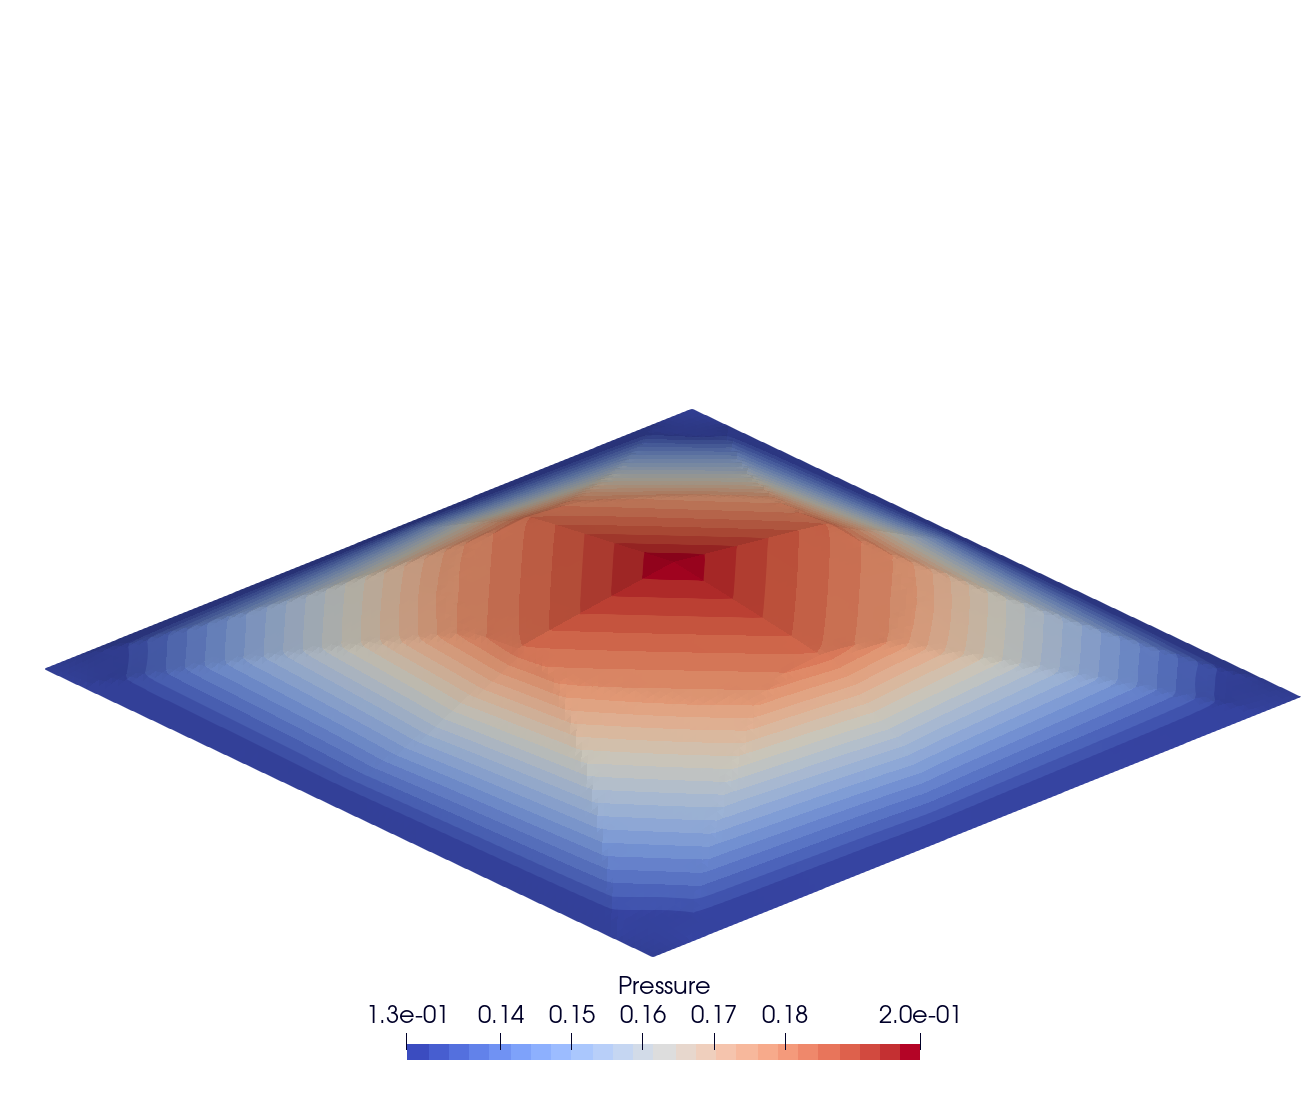
\includegraphics[width = 1.0\linewidth]{Figuras/Sensibilidade_malha_elemfin/pressure_wrapesc_Nsample4_Nxy100.png}
		\caption{$\text{N}_{x} = \text{N}_{y} = 100$.}
		\label{fig:pressure_wrapesc_Nsample4_Nxy100}
	\end{subfigure}
	\hfill
	\begin{subfigure}[b]{0.45\linewidth}
		\centering
		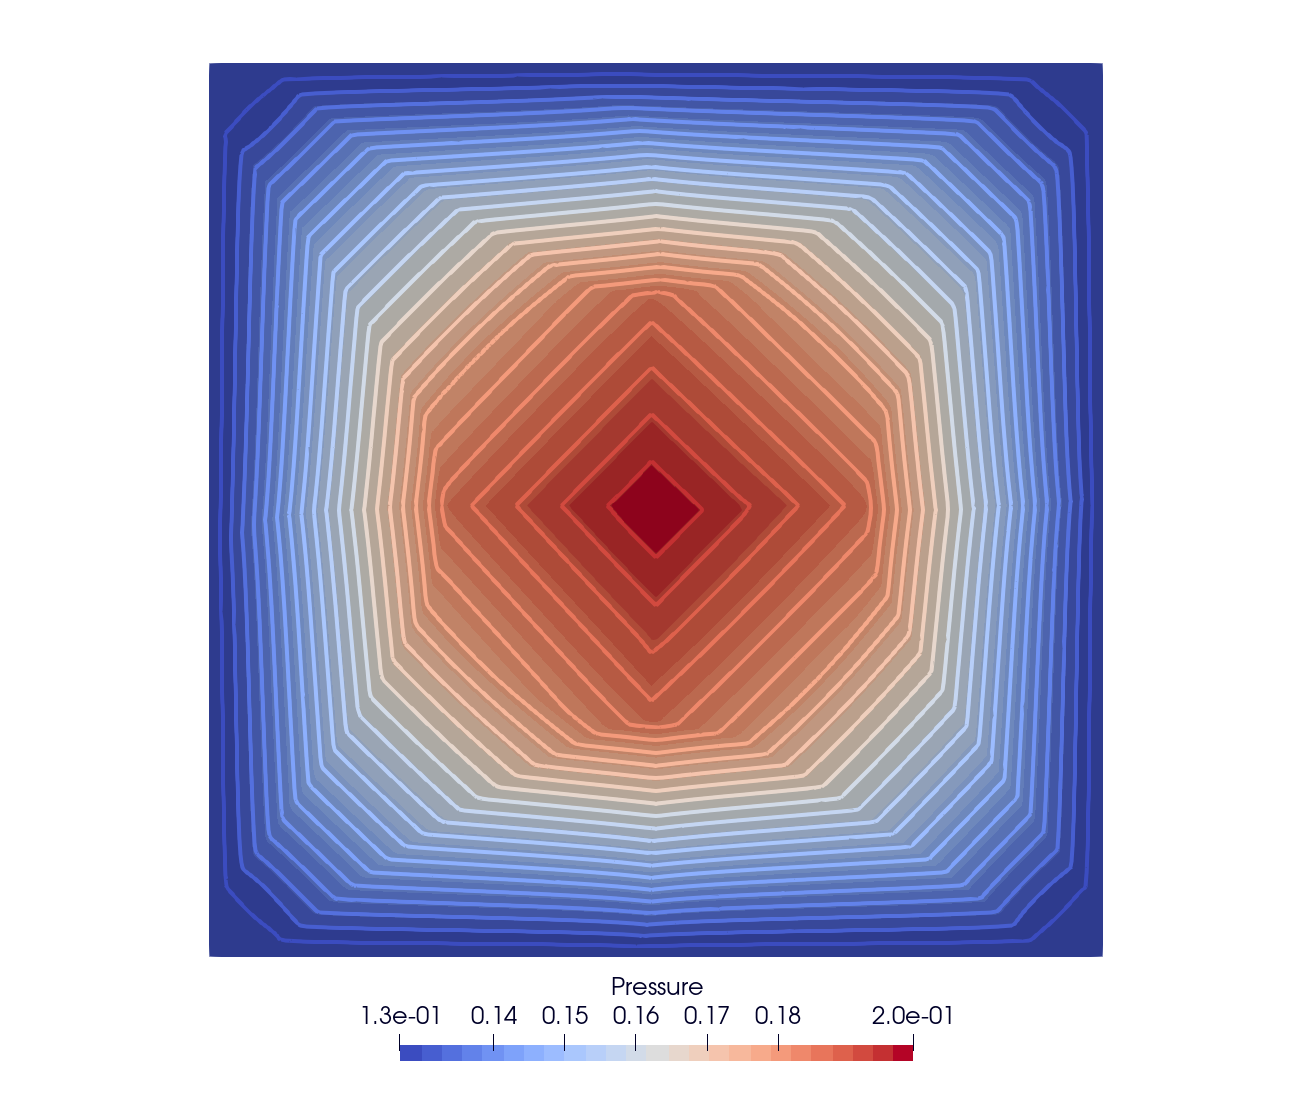
\includegraphics[width = 1.0\linewidth]{Figuras/Sensibilidade_malha_elemfin/pressure_contour_Nsample4_Nxy200.png}
		\caption{$\text{N}_{x} = \text{N}_{y} = 200$.}
		\label{fig:pressure_contour_Nsample4_Nxy200}
	\end{subfigure}
	\hfill
	\begin{subfigure}[b]{0.45\linewidth}
		\centering
		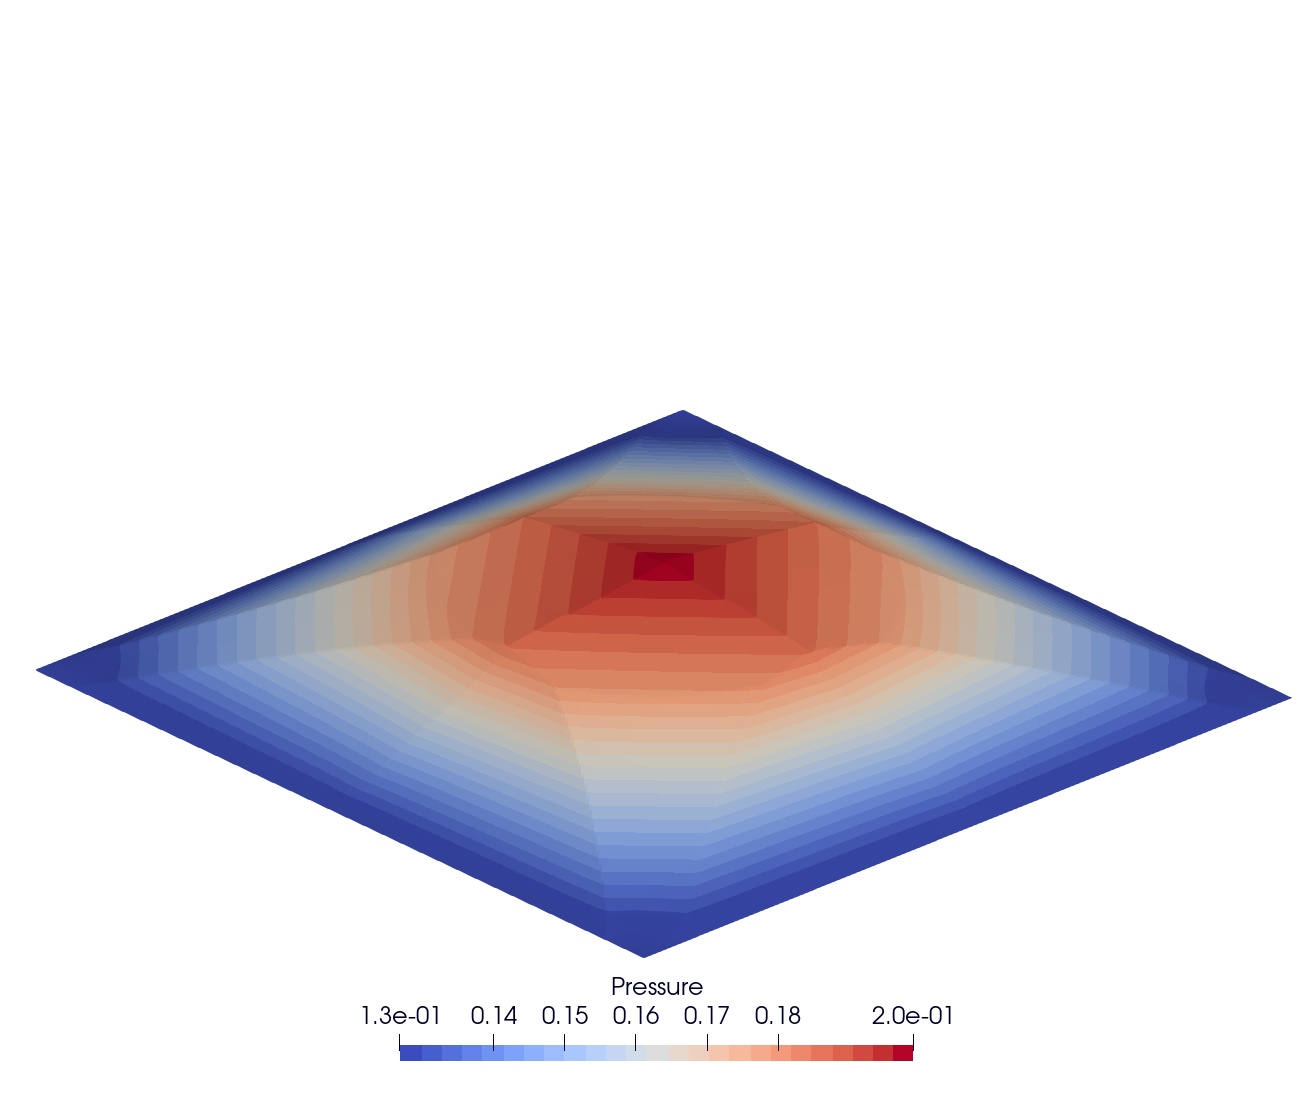
\includegraphics[width = 1.0\linewidth]{Figuras/Sensibilidade_malha_elemfin/pressure_wrapesc_Nsample4_Nxy200.png}
		\caption{$\text{N}_{x} = \text{N}_{y} = 200$.}
		\label{fig:pressure_wrapesc_Nsample4_Nxy200}
	\end{subfigure}
	\label{fig:pressure_mesh_fine}
\end{figure}

Os multiplicadores de Lagrange, denotados por $\lambda$, por sua vez, apresentam um comportamento semelhante. A bem da verdade, nota-se que a solução obtida aproxima-se daquela apresentada na figura \ref{fig:lambda_contour_NxNy101_Nsample4_4}. Para uma malhas de elementos finitos grosseiras (figura \ref{fig:lambda_mesh_coarse}), a solução apresenta variações pouco comportados, as quais são menos expressivas (ou imperceptíveis) quando malhas mais refinadas são empregadas (figura \ref{fig:lambda_mesh_fine}).

%lambda%
\begin{figure}[!ht]
	\centering
	\caption{À esquerda, curvas de nível do campo escalar dos multiplicadores de Lagrange, considerando $\text{N}_{x}^{\text{amostras}} = \text{N}_{y}^{\text{amostras}} = 4$ e malhas de elementos finitos grosseiras. À direita, as respectivas representações tridimensionais.}
	\begin{subfigure}[b]{0.45\linewidth}
		\centering
		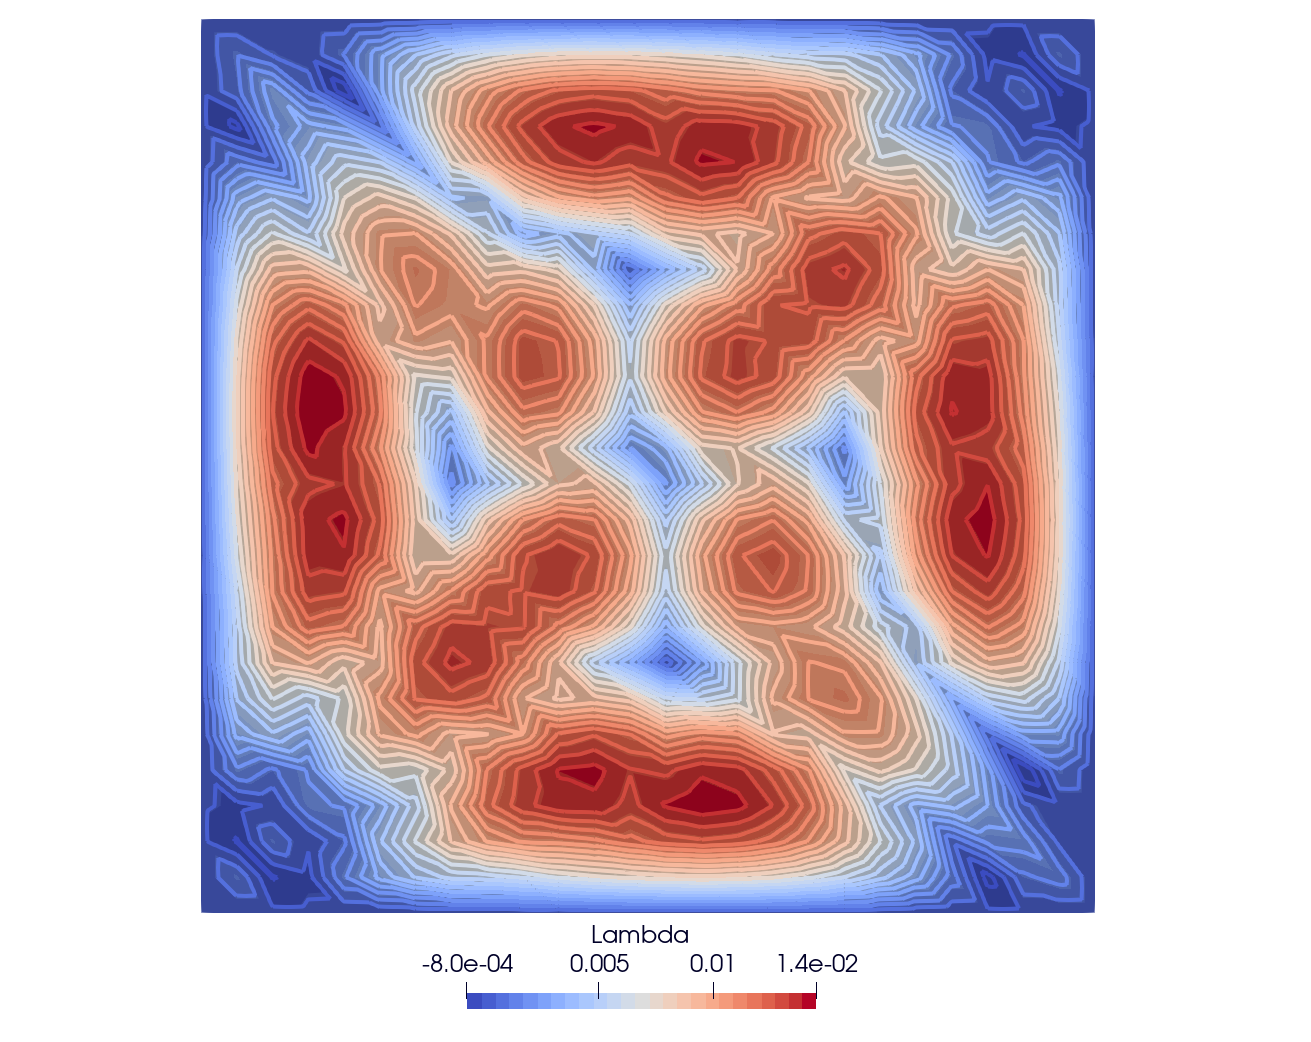
\includegraphics[width = 1.0\linewidth]{Figuras/Sensibilidade_malha_elemfin/lambda_contour_Nsample4_Nxy25.png}
		\caption{$\text{N}_{x} = \text{N}_{y} = 25$.}
		\label{fig:lambda_contour_Nsample4_Nxy25}
	\end{subfigure}
	\hfill
	\begin{subfigure}[b]{0.45\linewidth}
		\centering
		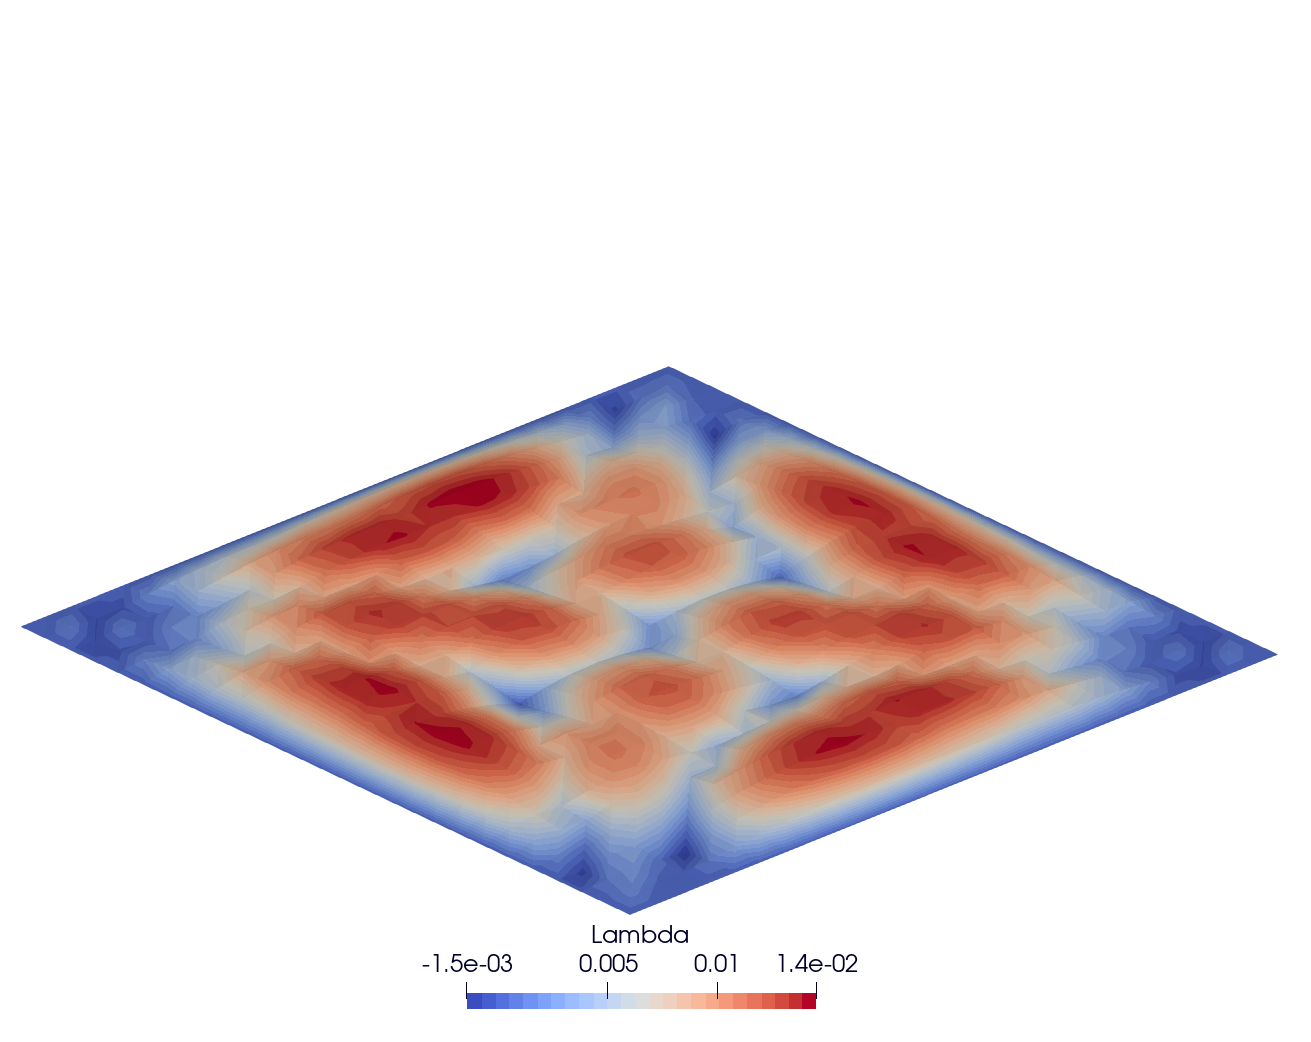
\includegraphics[width = 1.0\linewidth]{Figuras/Sensibilidade_malha_elemfin/lambda_wrapesc_Nsample4_Nxy25.png}
		\caption{$\text{N}_{x} = \text{N}_{y} = 25$.}
		\label{fig:lambda_wrapesc_Nsample4_Nxy25}
	\end{subfigure}
	\hfill
	\begin{subfigure}[b]{0.45\linewidth}
		\centering
		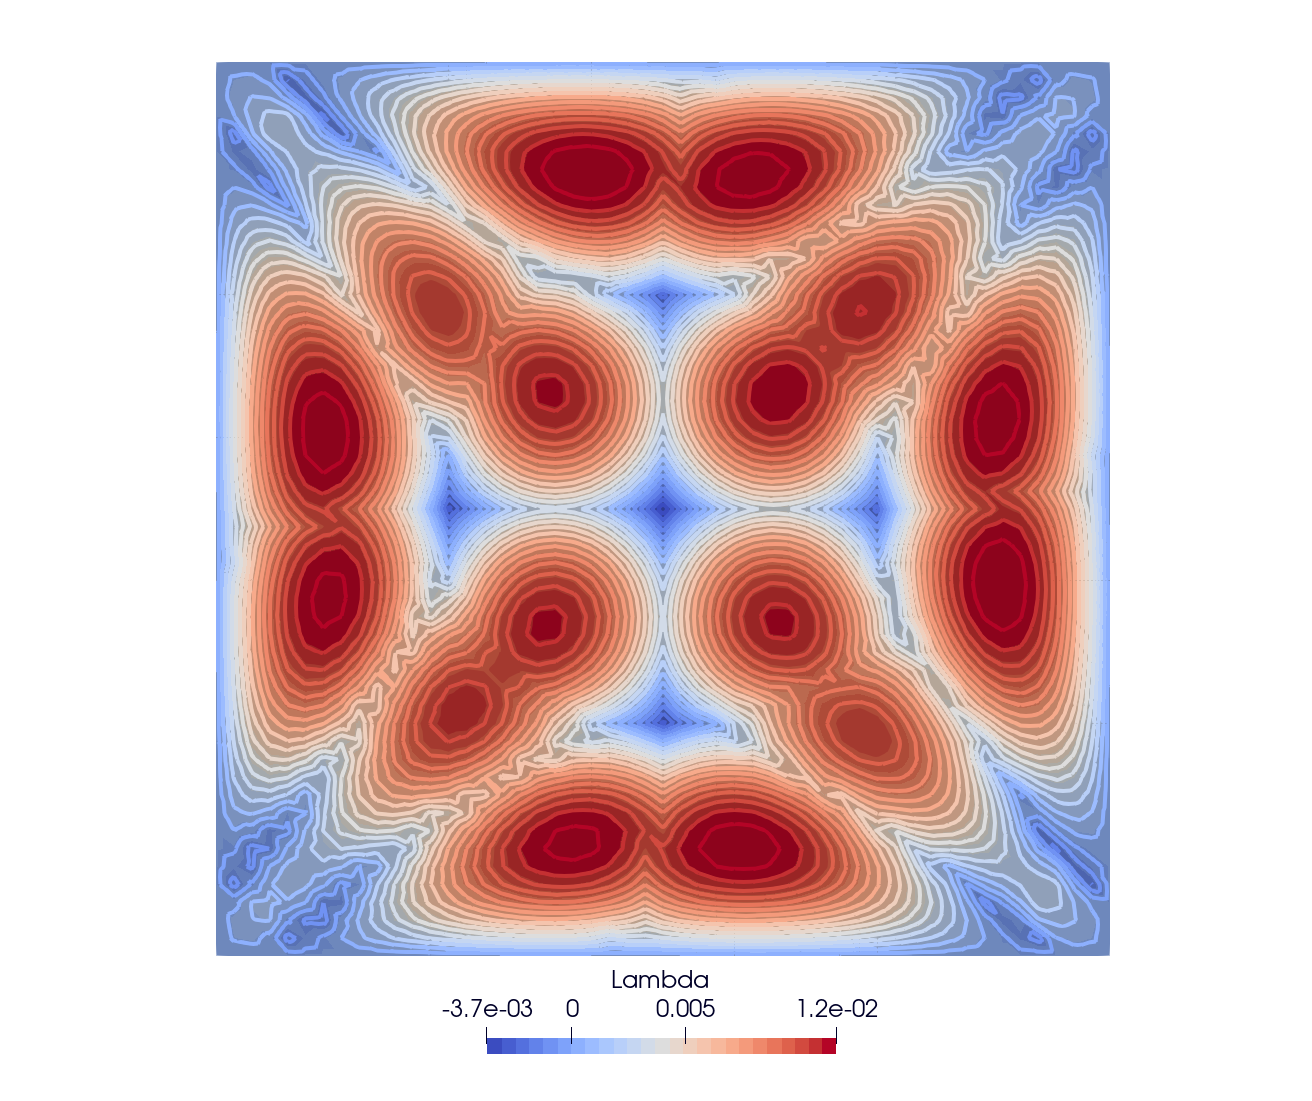
\includegraphics[width = 1.0\linewidth]{Figuras/Sensibilidade_malha_elemfin/lambda_contour_Nsample4_Nxy50.png}
		\caption{$\text{N}_{x} = \text{N}_{y} = 50$.}
		\label{fig:lambda_contour_Nsample4_Nxy50}
	\end{subfigure}
	\hfill
	\begin{subfigure}[b]{0.45\linewidth}
		\centering
		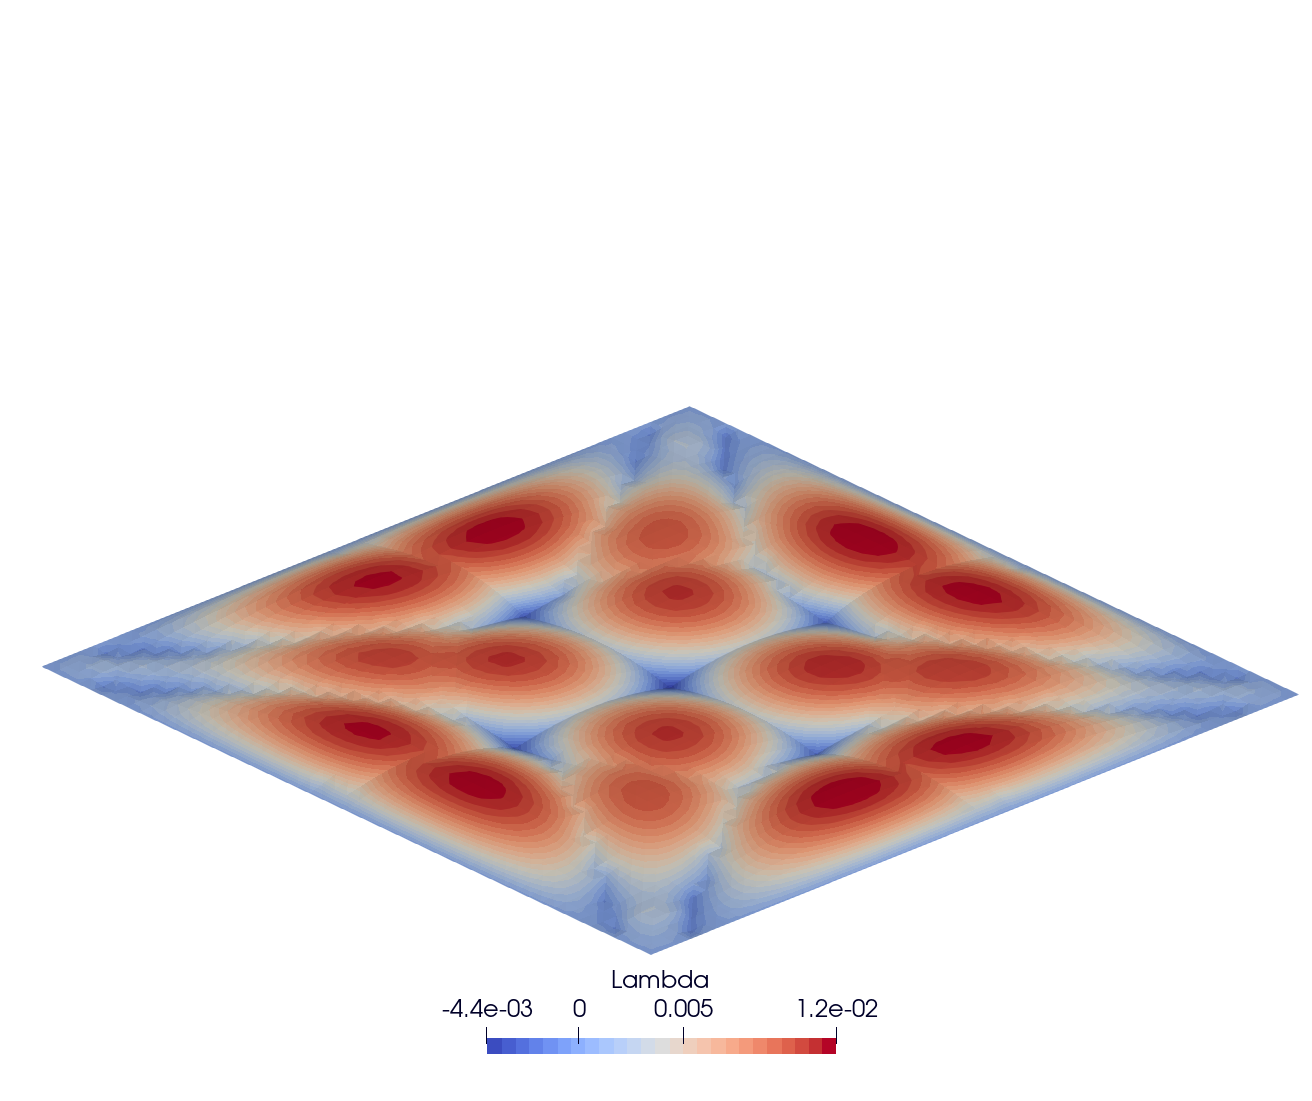
\includegraphics[width = 1.0\linewidth]{Figuras/Sensibilidade_malha_elemfin/lambda_wrapesc_Nsample4_Nxy50.png}
		\caption{$\text{N}_{x} = \text{N}_{y} = 50$.}
		\label{fig:lambda_wrapesc_Nsample4_Nxy50}
	\end{subfigure}
	\label{fig:lambda_mesh_coarse}
\end{figure}

Em relação ao fluxo, $\mathbf{u}$, tem-se, novamente, um comportamento análogo aos discutidos anteriormente. Ao comparar os resultados apresentados nas figuras \ref{fig:pressure_mesh_coarse} e \ref{fig:pressure_mesh_fine} com aqueles ilustrados na figura \ref{fig:flux_mesh}, nota-se que a lei de Darcy (equação (3.11) é respeitada, ou seja, o fluxo, $\mathbf{u}$ -- também denominada por $\mathbf{q}$ -- é contrário ao gradiente de pressão, $\nabla p$.  

\begin{figure}[!ht]
	\centering
	\caption{À esquerda, curvas de nível do campo escalar dos multiplicadores de Lagrange, considerando $\text{N}_{x}^{\text{amostras}} = \text{N}_{y}^{\text{amostras}} = 4$ e malhas de elementos finitos refinadas. À direita, as respectivas representações tridimensionais.}
	\begin{subfigure}[b]{0.45\linewidth}
		\centering
		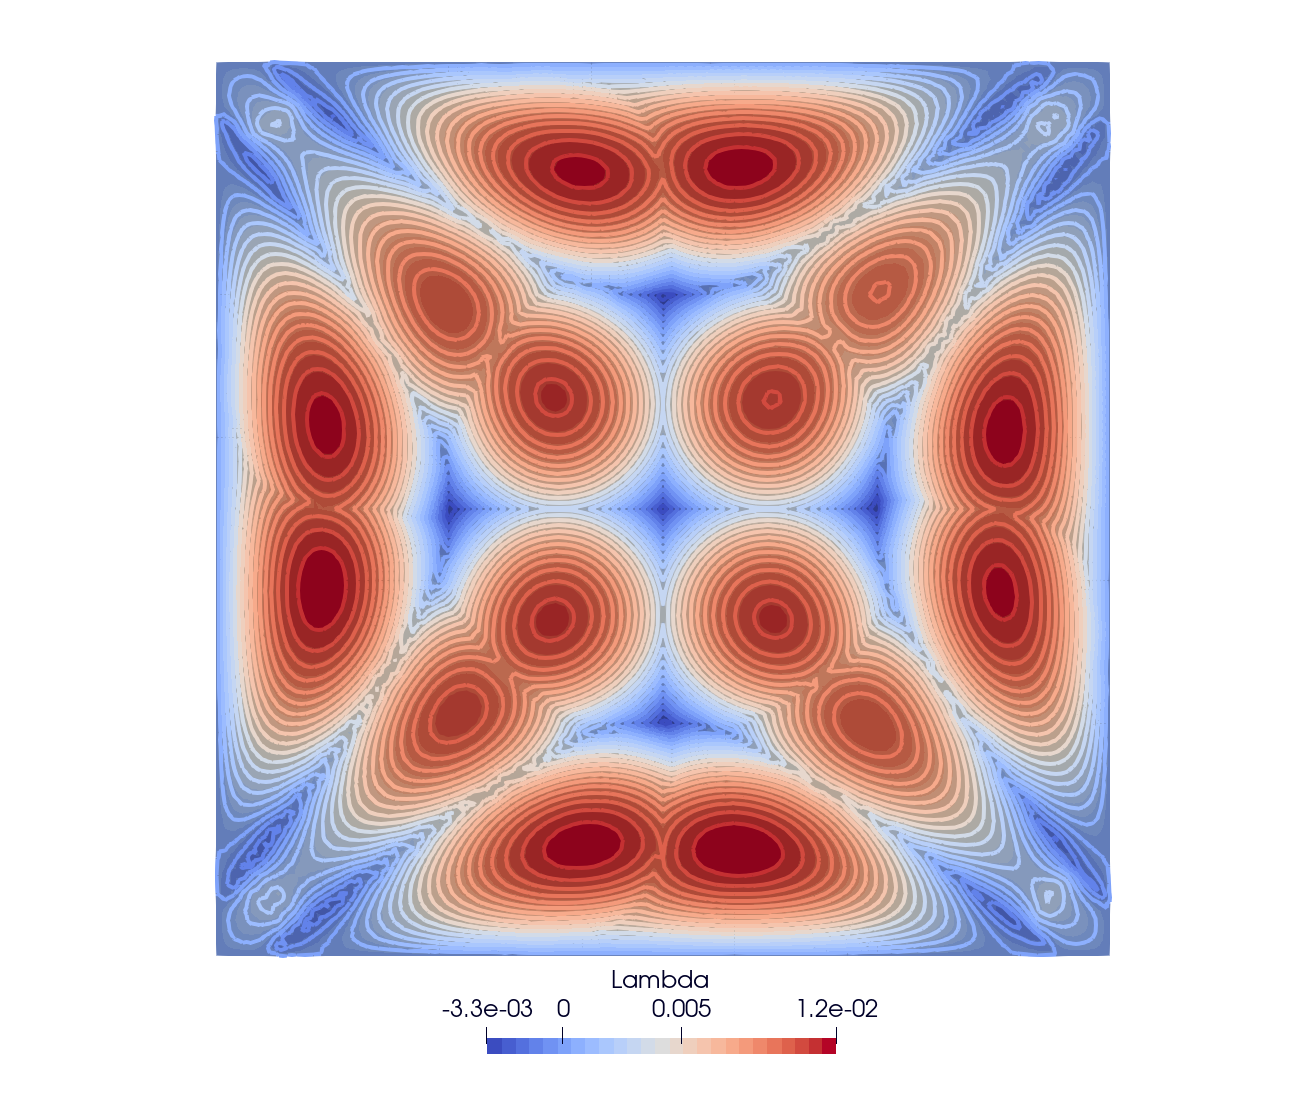
\includegraphics[width = 1.0\linewidth]{Figuras/Sensibilidade_malha_elemfin/lambda_contour_Nsample4_Nxy100.png}
		\caption{$\text{N}_{x} = \text{N}_{y} = 100$.}
		\label{fig:lambda_contour_Nsample4_Nxy100}
	\end{subfigure}
	\hfill
	\begin{subfigure}[b]{0.45\linewidth}
		\centering
		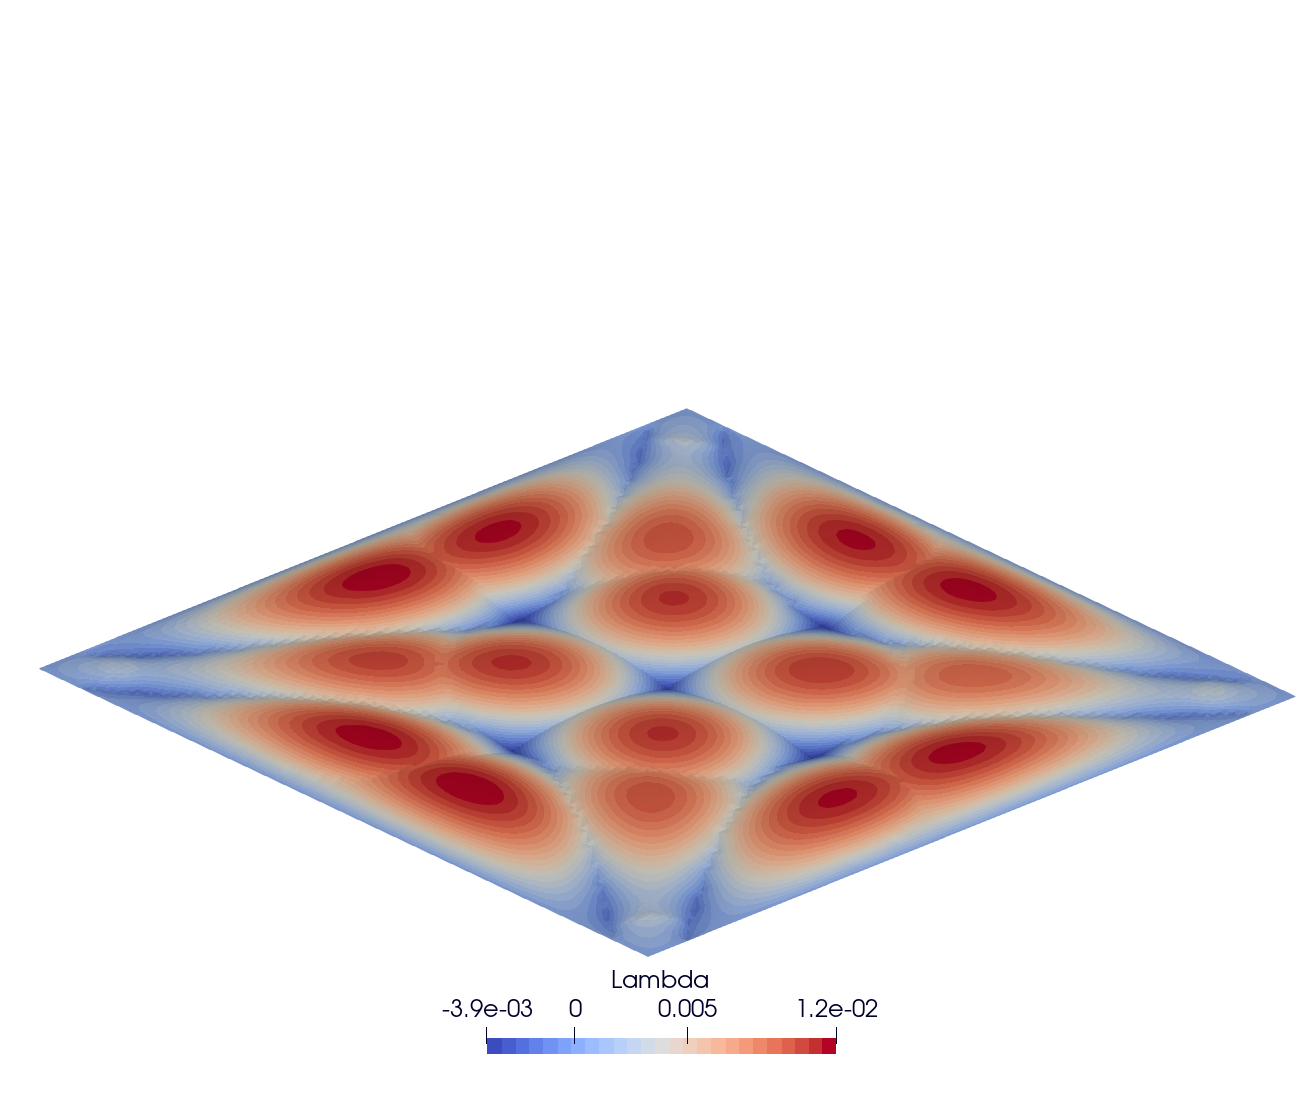
\includegraphics[width = 1.0\linewidth]{Figuras/Sensibilidade_malha_elemfin/lambda_wrapesc_Nsample4_Nxy100.png}
		\caption{$\text{N}_{x} = \text{N}_{y} = 100$.}
		\label{fig:lambda_wrapesc_Nsample4_Nxy100}
	\end{subfigure}
	\hfill
	\begin{subfigure}[b]{0.45\linewidth}
		\centering
		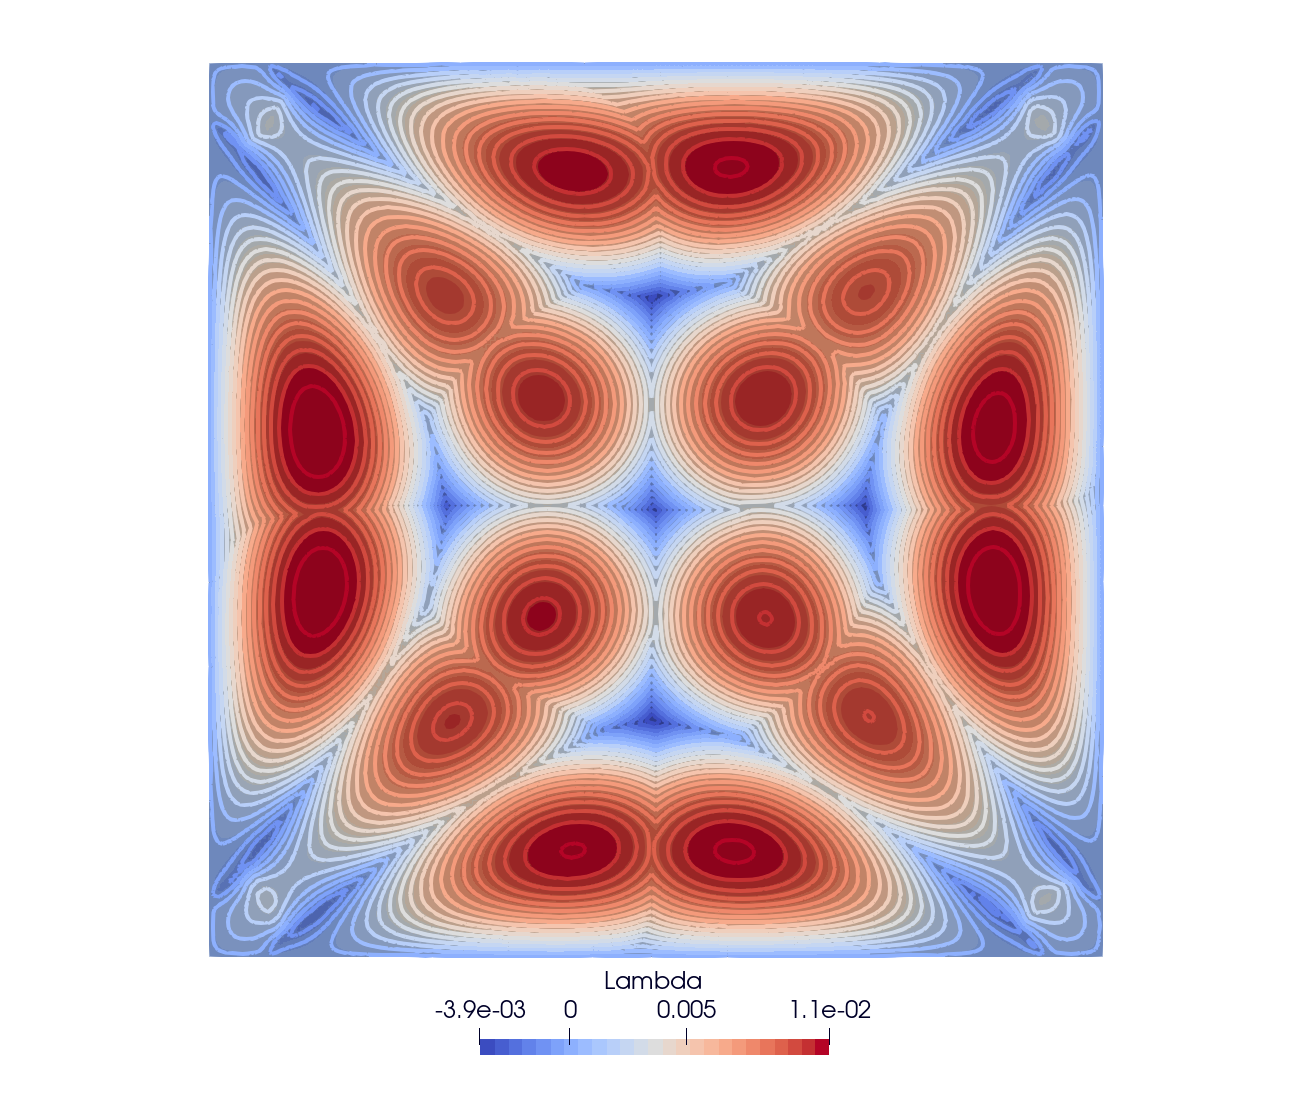
\includegraphics[width = 1.0\linewidth]{Figuras/Sensibilidade_malha_elemfin/lambda_contour_Nsample4_Nxy200.png}
		\caption{$\text{N}_{x} = \text{N}_{y} = 200$.}
		\label{fig:lambda_contour_Nsample4_Nxy200}
	\end{subfigure}
	\hfill
	\begin{subfigure}[b]{0.45\linewidth}
		\centering
		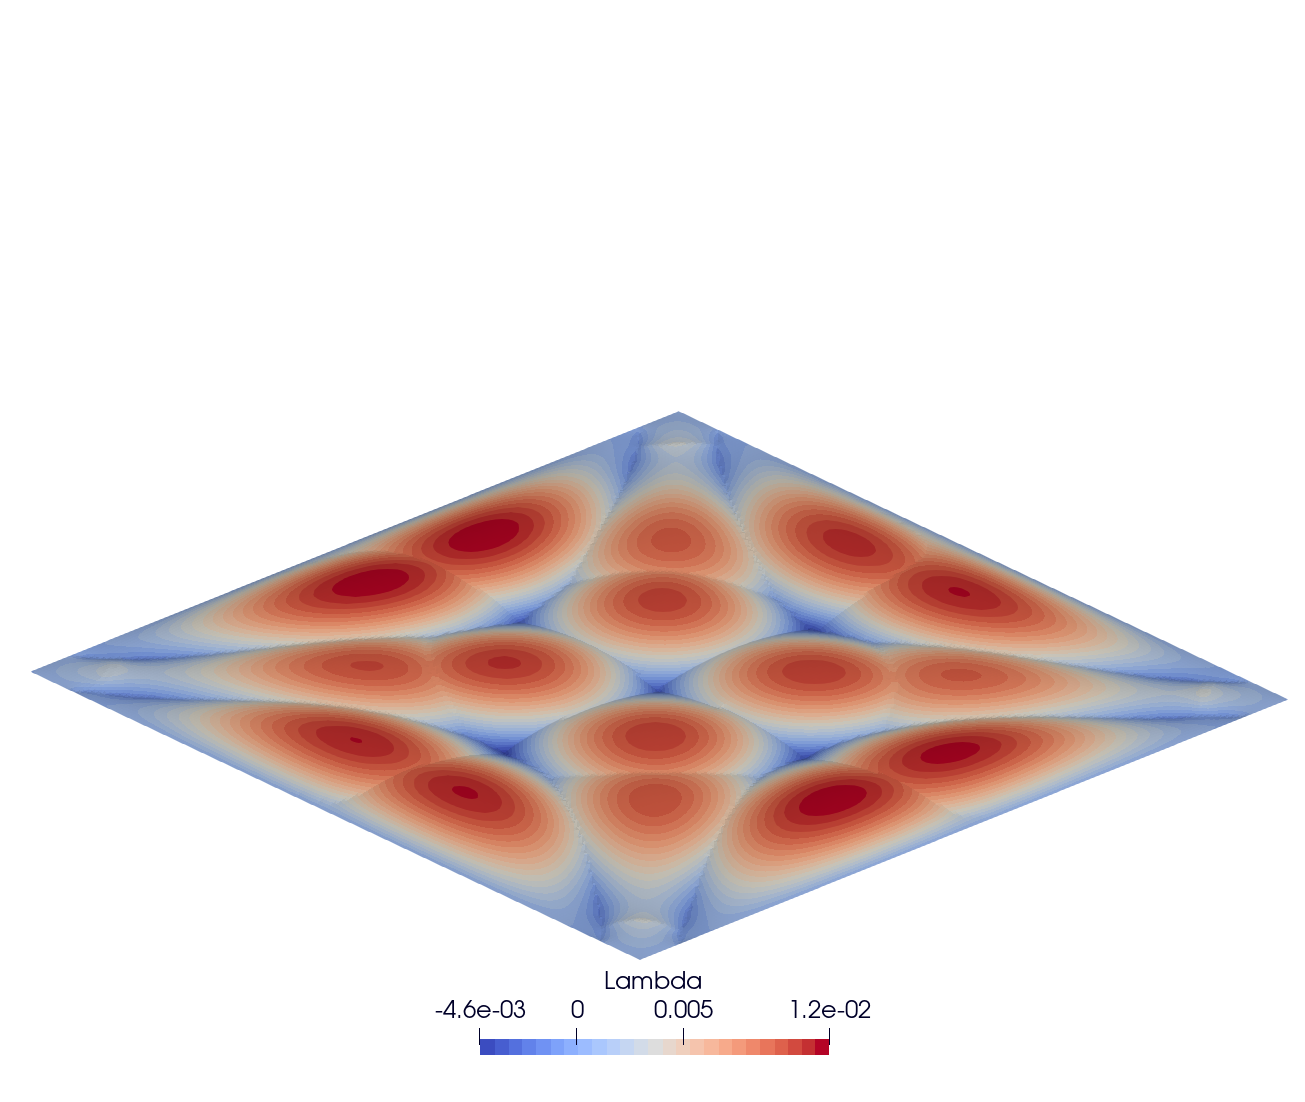
\includegraphics[width = 1.0\linewidth]{Figuras/Sensibilidade_malha_elemfin/lambda_wrapesc_Nsample4_Nxy200.png}
		\caption{$\text{N}_{x} = \text{N}_{y} = 200$.}
		\label{fig:lambda_wrapesc_Nsample4_Nxy200}
	\end{subfigure}
	\label{fig:lambda_mesh_fine}
\end{figure}

%Flux%
\begin{figure}[!ht]
	\centering
	\caption{Fluxo, $\mathbf{u}$, considerando $\text{N}_{x}^{\text{amostras}} = \text{N}_{y}^{\text{amostras}} = 4$ e diferentes malhas de elementos finitos.}
	\begin{subfigure}[b]{0.45\linewidth}
		\centering
		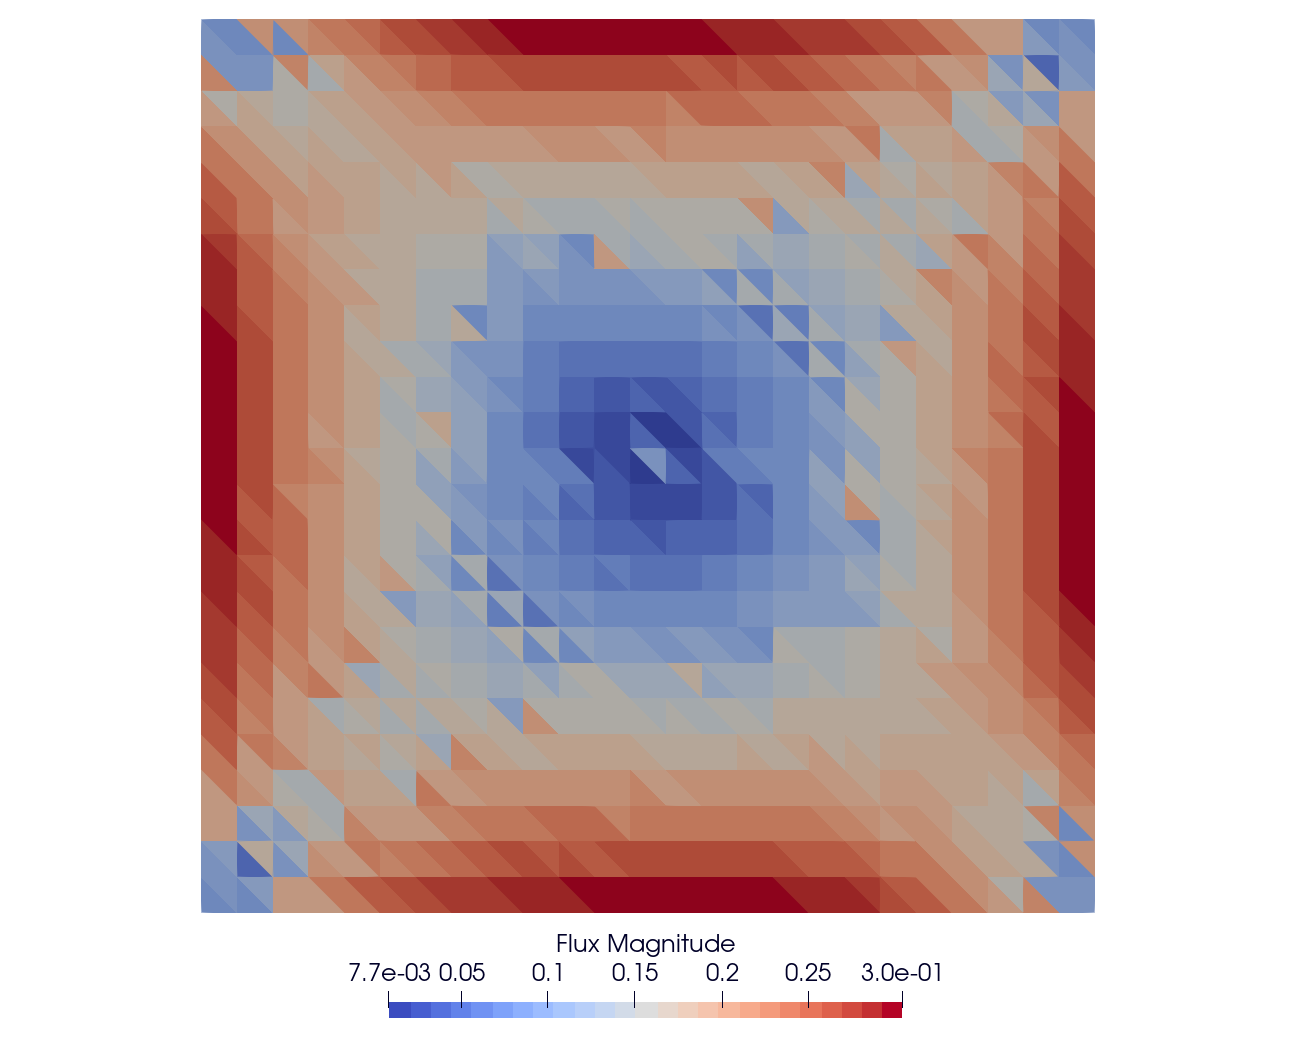
\includegraphics[width = 1.0\linewidth]{Figuras/Sensibilidade_malha_elemfin/flux_Nsample4_Nxy25.png}
		\caption{$\text{N}_{x} = \text{N}_{y} = 25$.}
		\label{fig:flux_Nsample4_Nxy25}
	\end{subfigure}
	\hfill
	\begin{subfigure}[b]{0.45\linewidth}
		\centering
		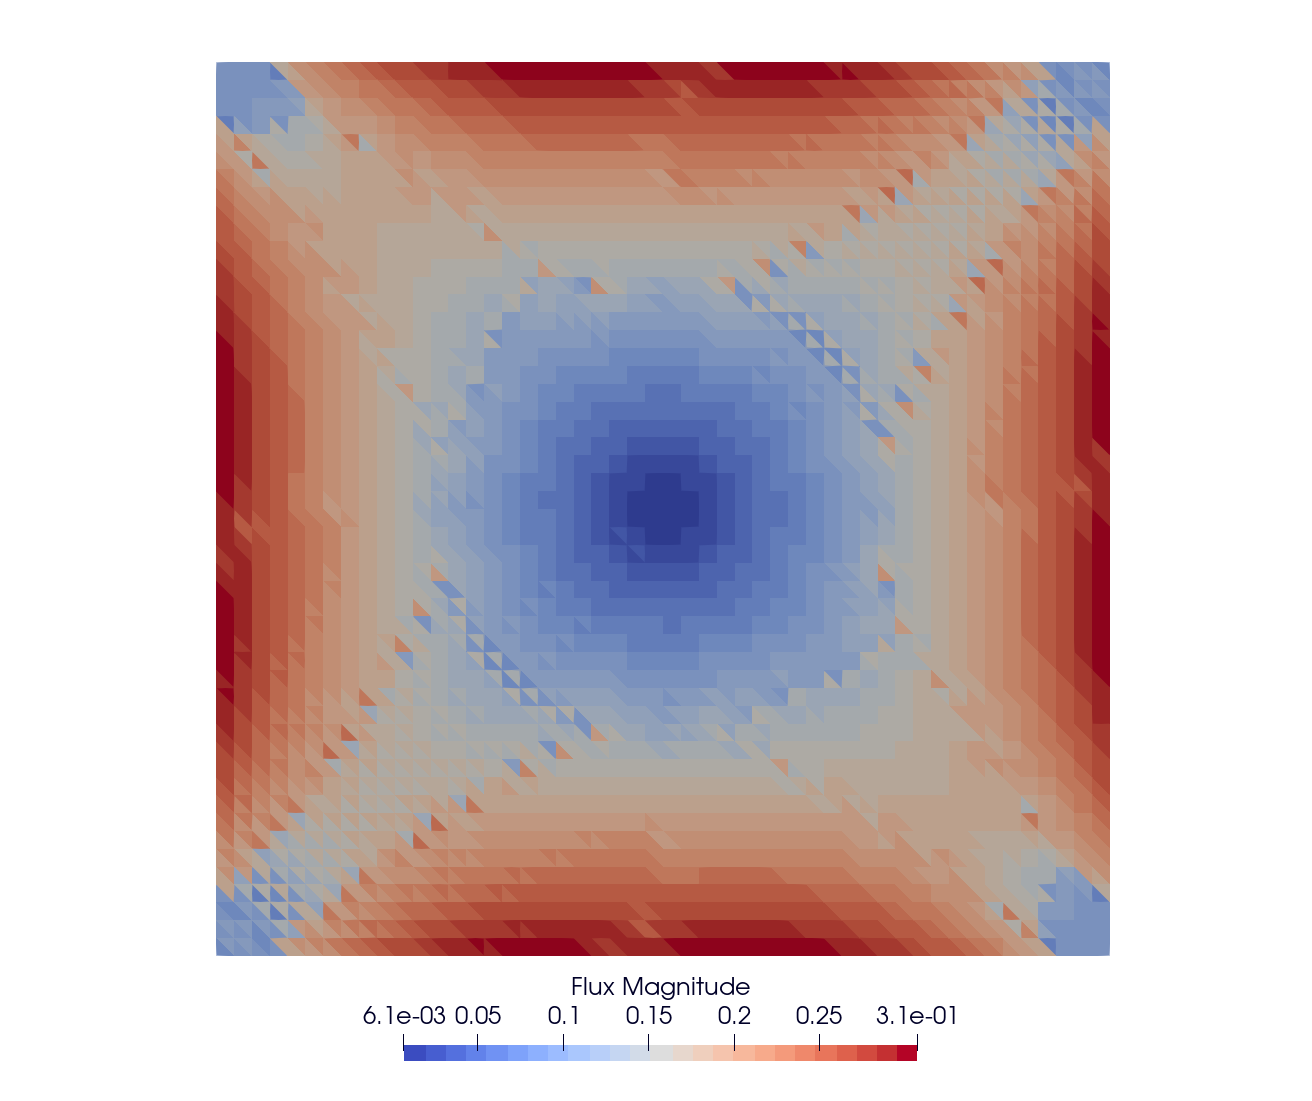
\includegraphics[width = 1.0\linewidth]{Figuras/Sensibilidade_malha_elemfin/flux_Nsample4_Nxy50.png}
		\caption{$\text{N}_{x} = \text{N}_{y} = 50$.}
		\label{fig:flux_Nsample4_Nxy50}
	\end{subfigure}
	\hfill
	\begin{subfigure}[b]{0.45\linewidth}
		\centering
		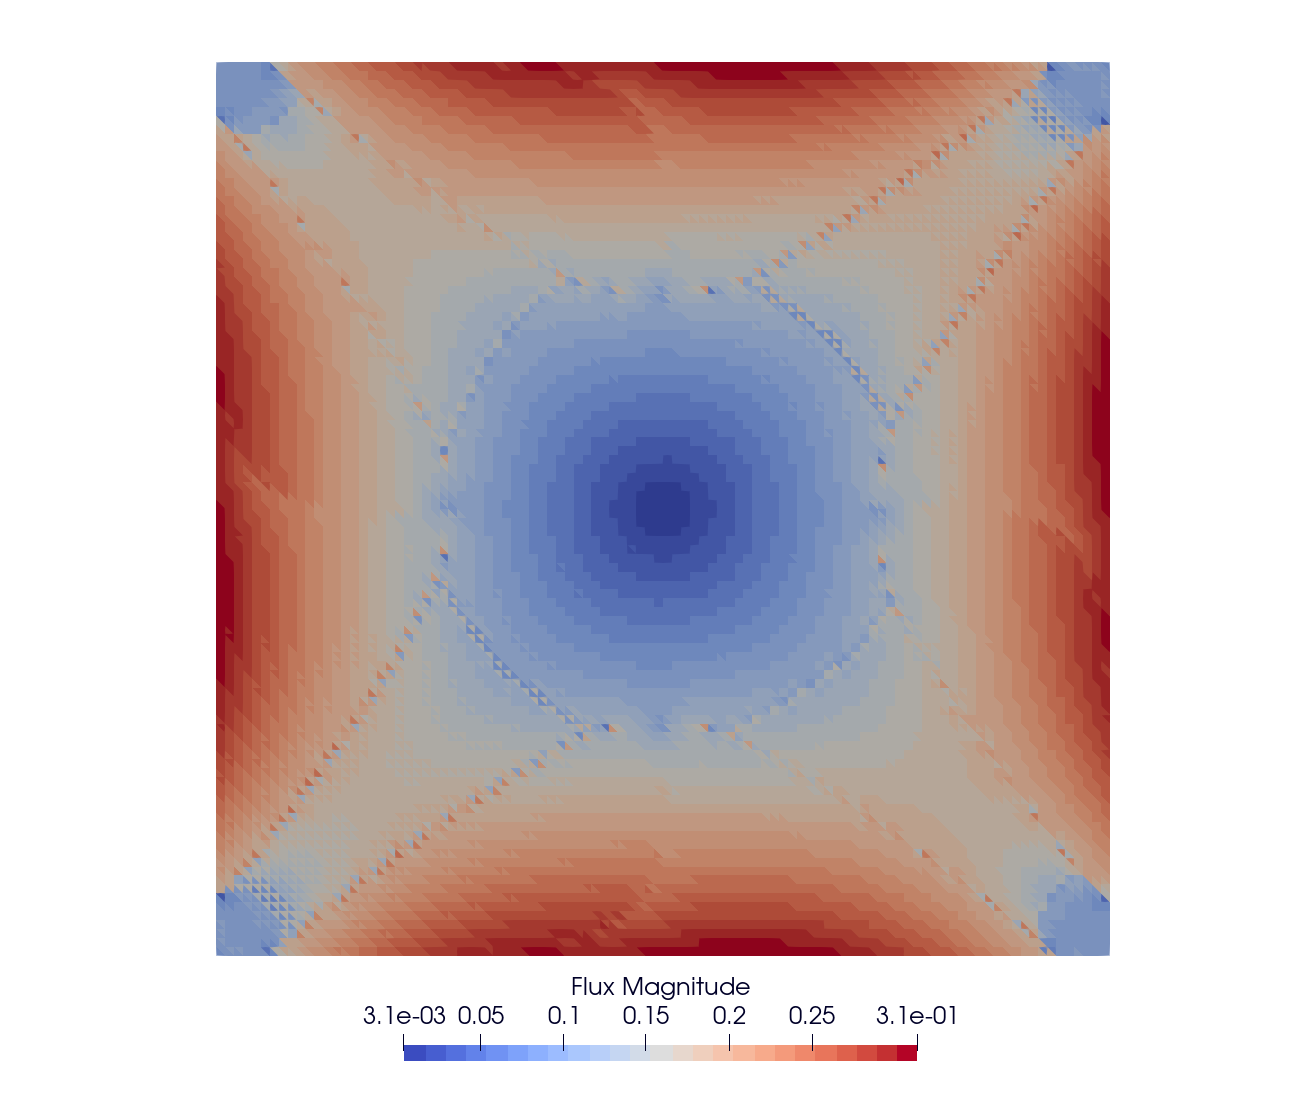
\includegraphics[width = 1.0\linewidth]{Figuras/Sensibilidade_malha_elemfin/flux_Nsample4_Nxy100.png}
		\caption{$\text{N}_{x} = \text{N}_{y} = 100$.}
		\label{fig:flux_Nsample4_Nxy100}
	\end{subfigure}
	\hfill
	\begin{subfigure}[b]{0.45\linewidth}
		\centering
		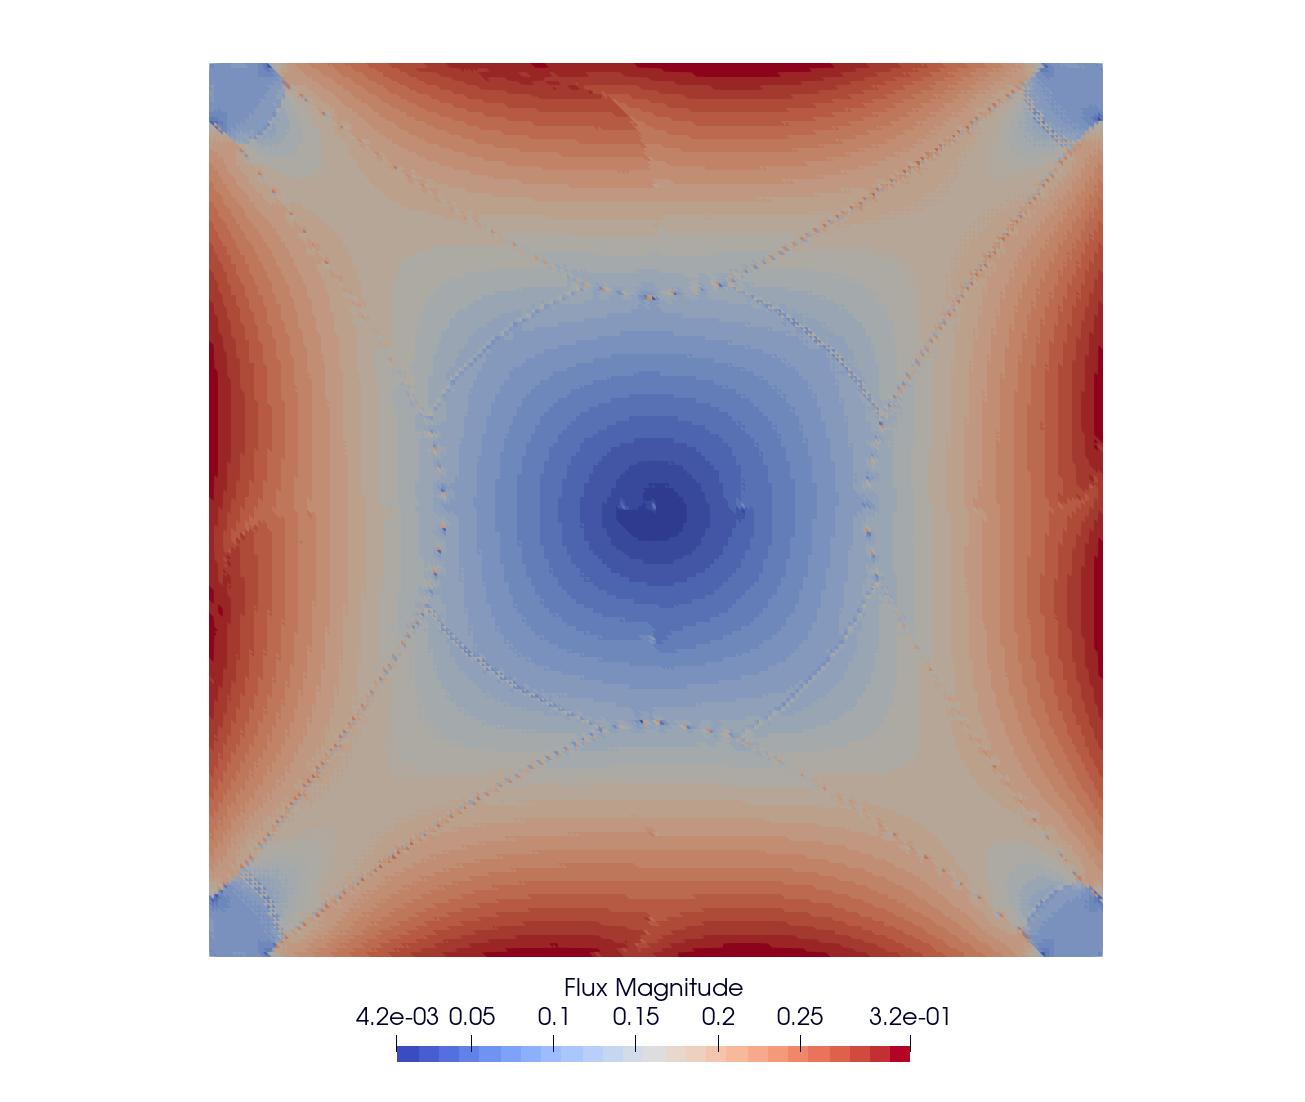
\includegraphics[width = 1.0\linewidth]{Figuras/Sensibilidade_malha_elemfin/flux_Nsample4_Nxy200.png}
		\caption{$\text{N}_{x} = \text{N}_{y} = 200$.}
		\label{fig:flux_Nsample4_Nxy200}
	\end{subfigure}
	\label{fig:flux_mesh}
\end{figure}

%mu%
\begin{figure}[!ht]
	\centering
	\caption{$\boldsymbol{\mu}$ considerando $\text{N}_{x}^{\text{amostras}} = \text{N}_{y}^{\text{amostras}} = 4$ e diferentes malhas de elementos finitos.}
	\begin{subfigure}[b]{0.45\linewidth}
		\centering
		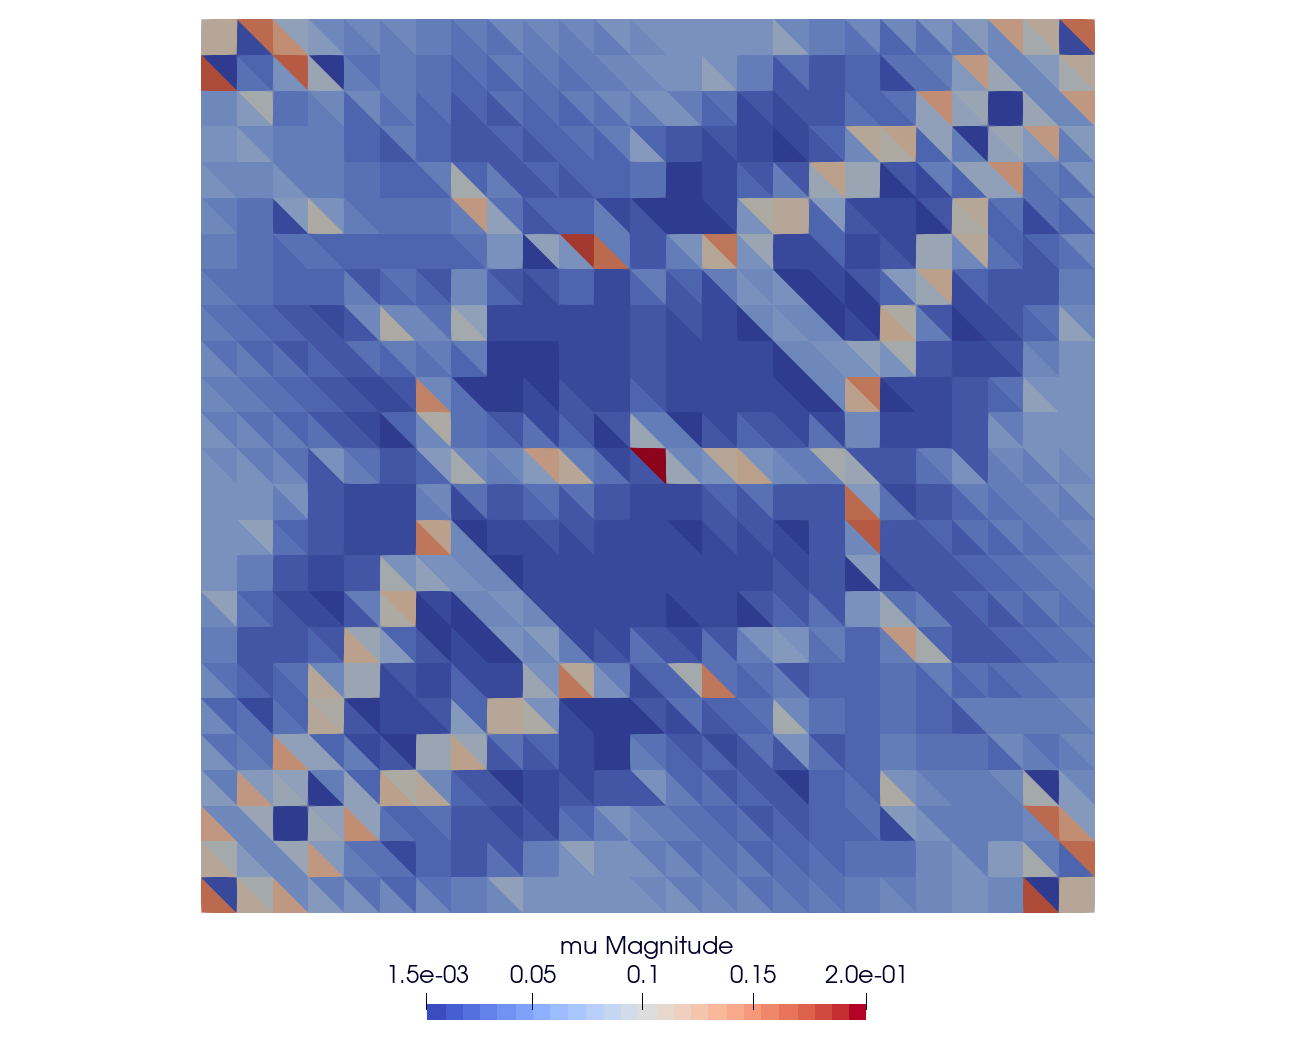
\includegraphics[width = 1.0\linewidth]{Figuras/Sensibilidade_malha_elemfin/mu_Nsample4_Nxy25.png}
		\caption{$\text{N}_{x} = \text{N}_{y} = 25$.}
		\label{fig:mu_Nsample4_Nxy25}
	\end{subfigure}
	\hfill
	\begin{subfigure}[b]{0.45\linewidth}
		\centering
		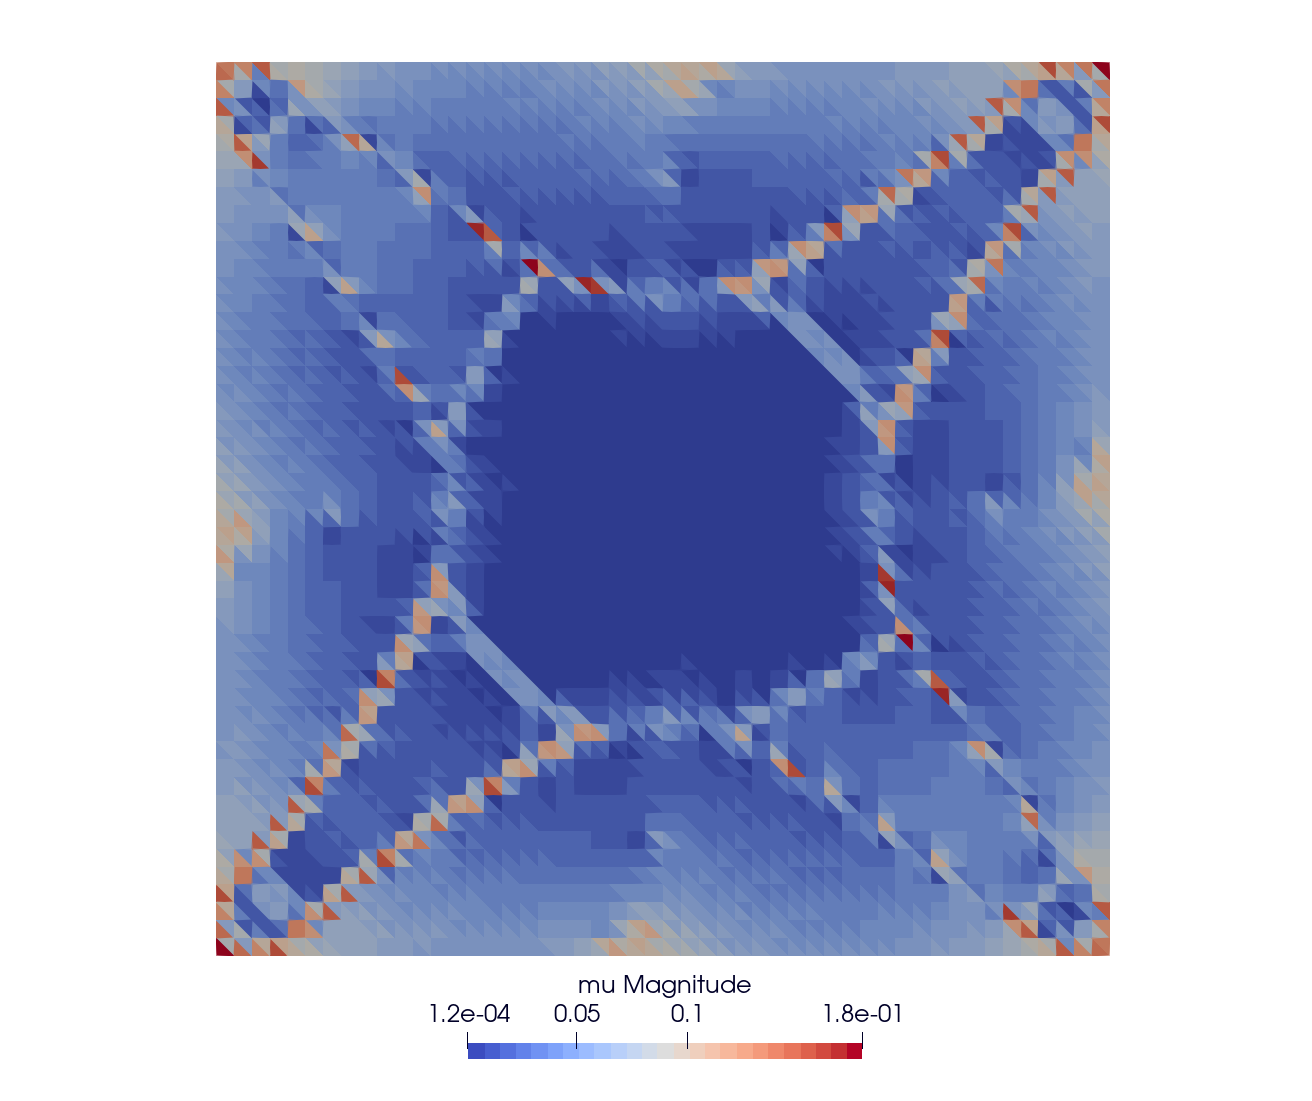
\includegraphics[width = 1.0\linewidth]{Figuras/Sensibilidade_malha_elemfin/mu_Nsample4_Nxy50.png}
		\caption{$\text{N}_{x} = \text{N}_{y} = 50$.}
		\label{fig:mu_Nsample4_Nxy50}
	\end{subfigure}
	\hfill
	\begin{subfigure}[b]{0.45\linewidth}
		\centering
		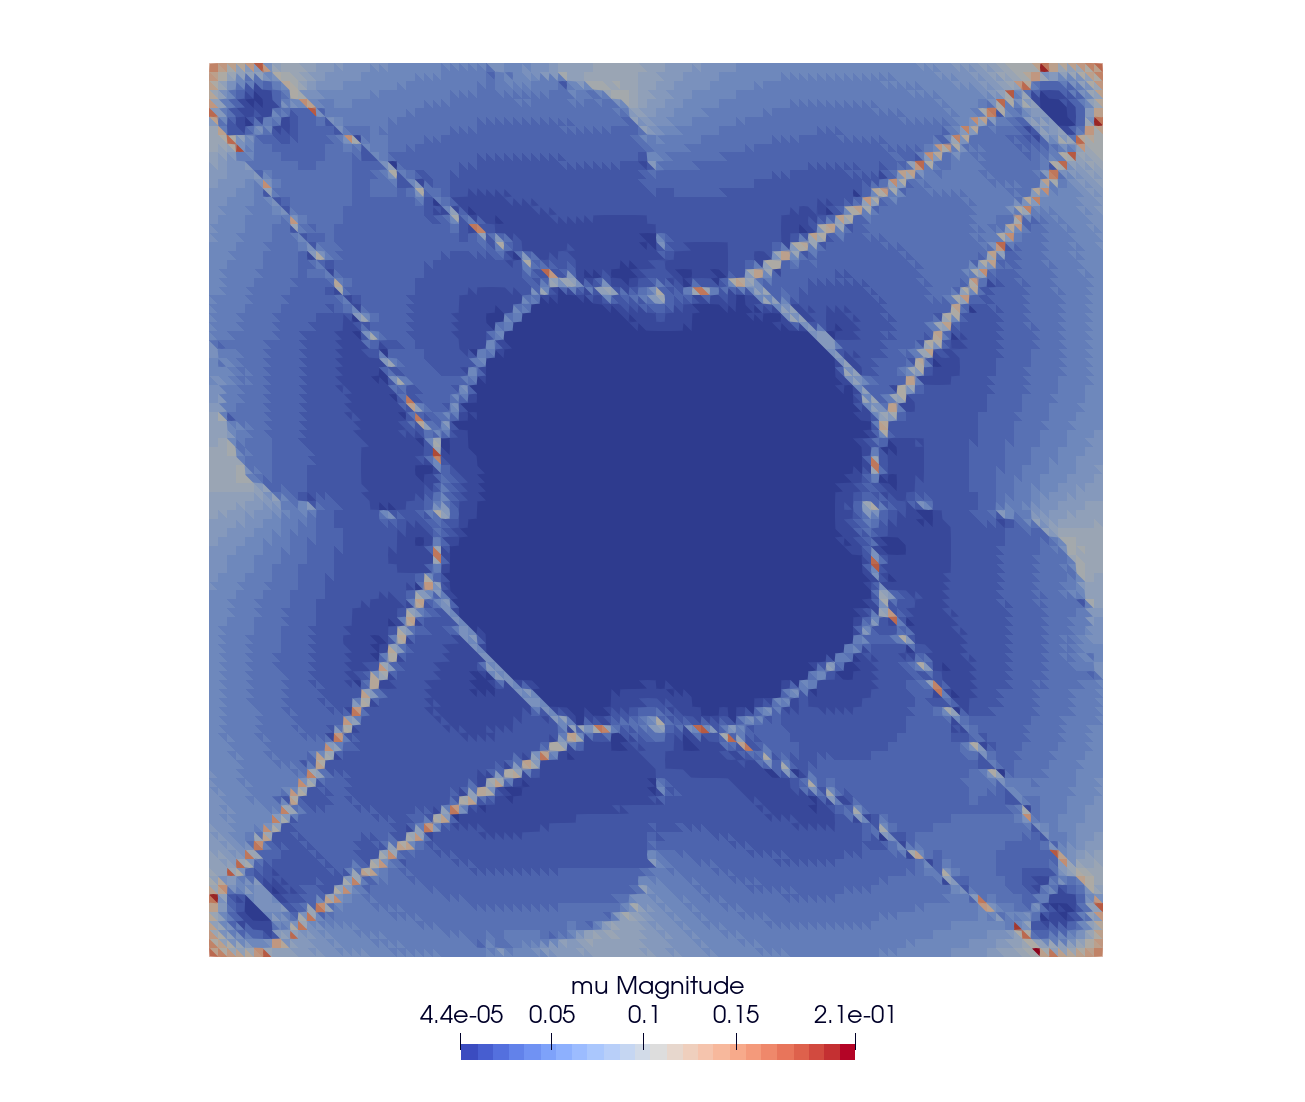
\includegraphics[width = 1.0\linewidth]{Figuras/Sensibilidade_malha_elemfin/mu_Nsample4_Nxy100.png}
		\caption{$\text{N}_{x} = \text{N}_{y} = 100$.}
		\label{fig:mu_Nsample4_Nxy100}
	\end{subfigure}
	\hfill
	\begin{subfigure}[b]{0.45\linewidth}
		\centering
		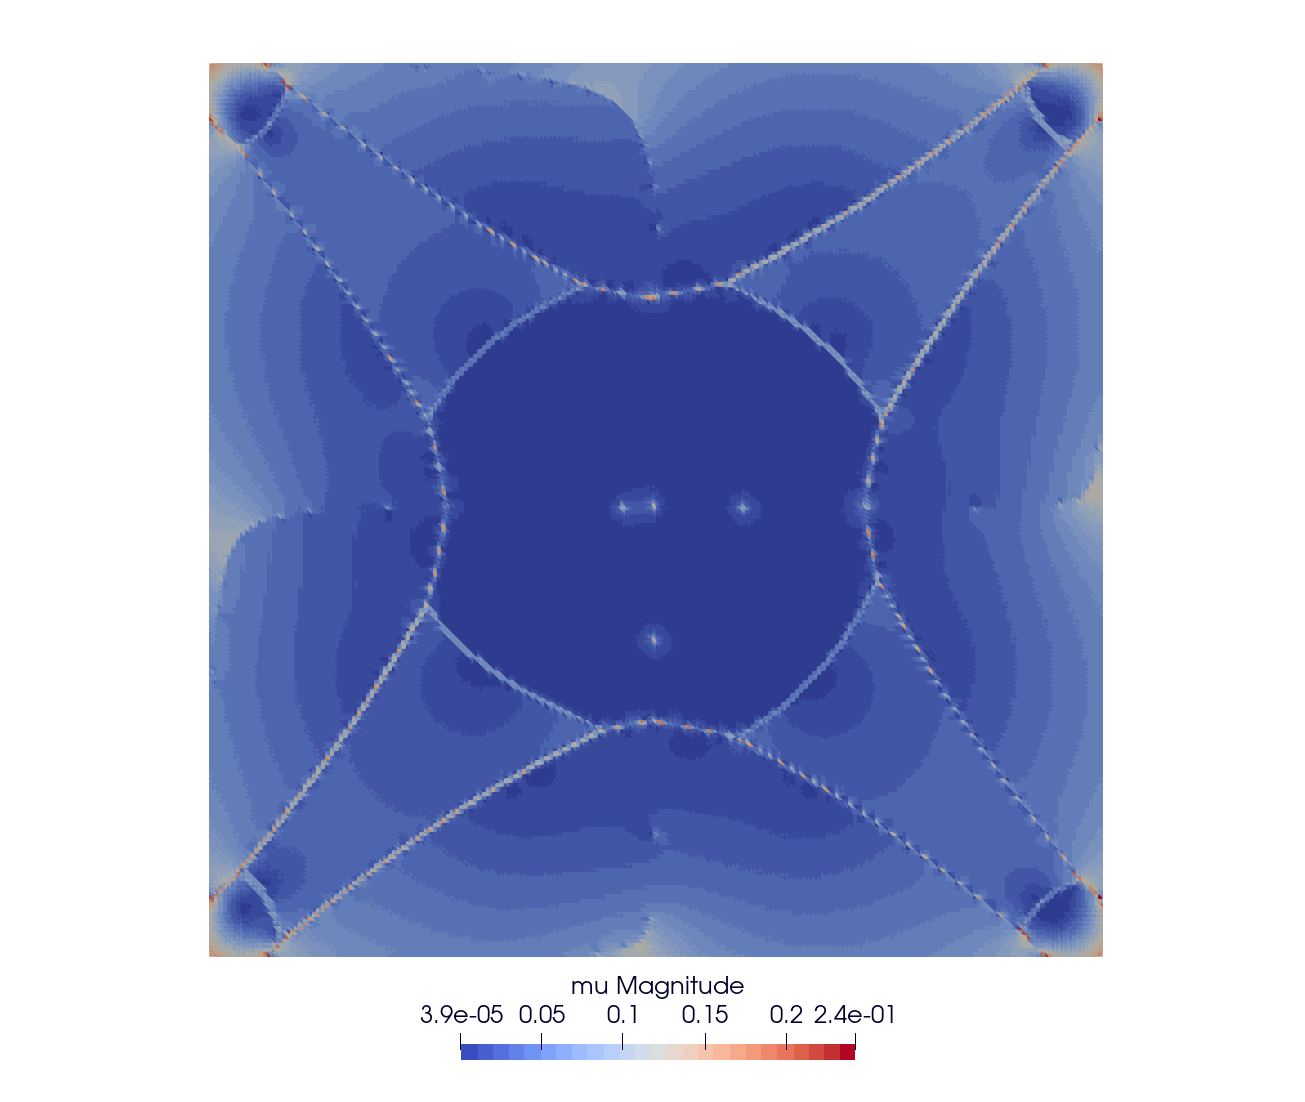
\includegraphics[width = 1.0\linewidth]{Figuras/Sensibilidade_malha_elemfin/mu_Nsample4_Nxy200.png}
		\caption{$\text{N}_{x} = \text{N}_{y} = 200$.}
		\label{fig:mu_Nsample4_Nxy200}
	\end{subfigure}
	\label{fig:mu_mesh}
\end{figure}

\clearpage
\subsection{Análise de convergência em relação ao número de pontos amostrais}

\subsubsection{Permeabilidade homogênea e unitária}

\begin{figure}[!ht]
	\centering
	\caption{Análise de convergência do campo escalar de pressões e do fluxo de Darcy em relação do número de pontos amostrais, em uma malha de elementos finitos $20 \times 20$ e um campo de permeabilidade homogêneo.}
	\begin{subfigure}[t]{0.45\linewidth}
		\centering
		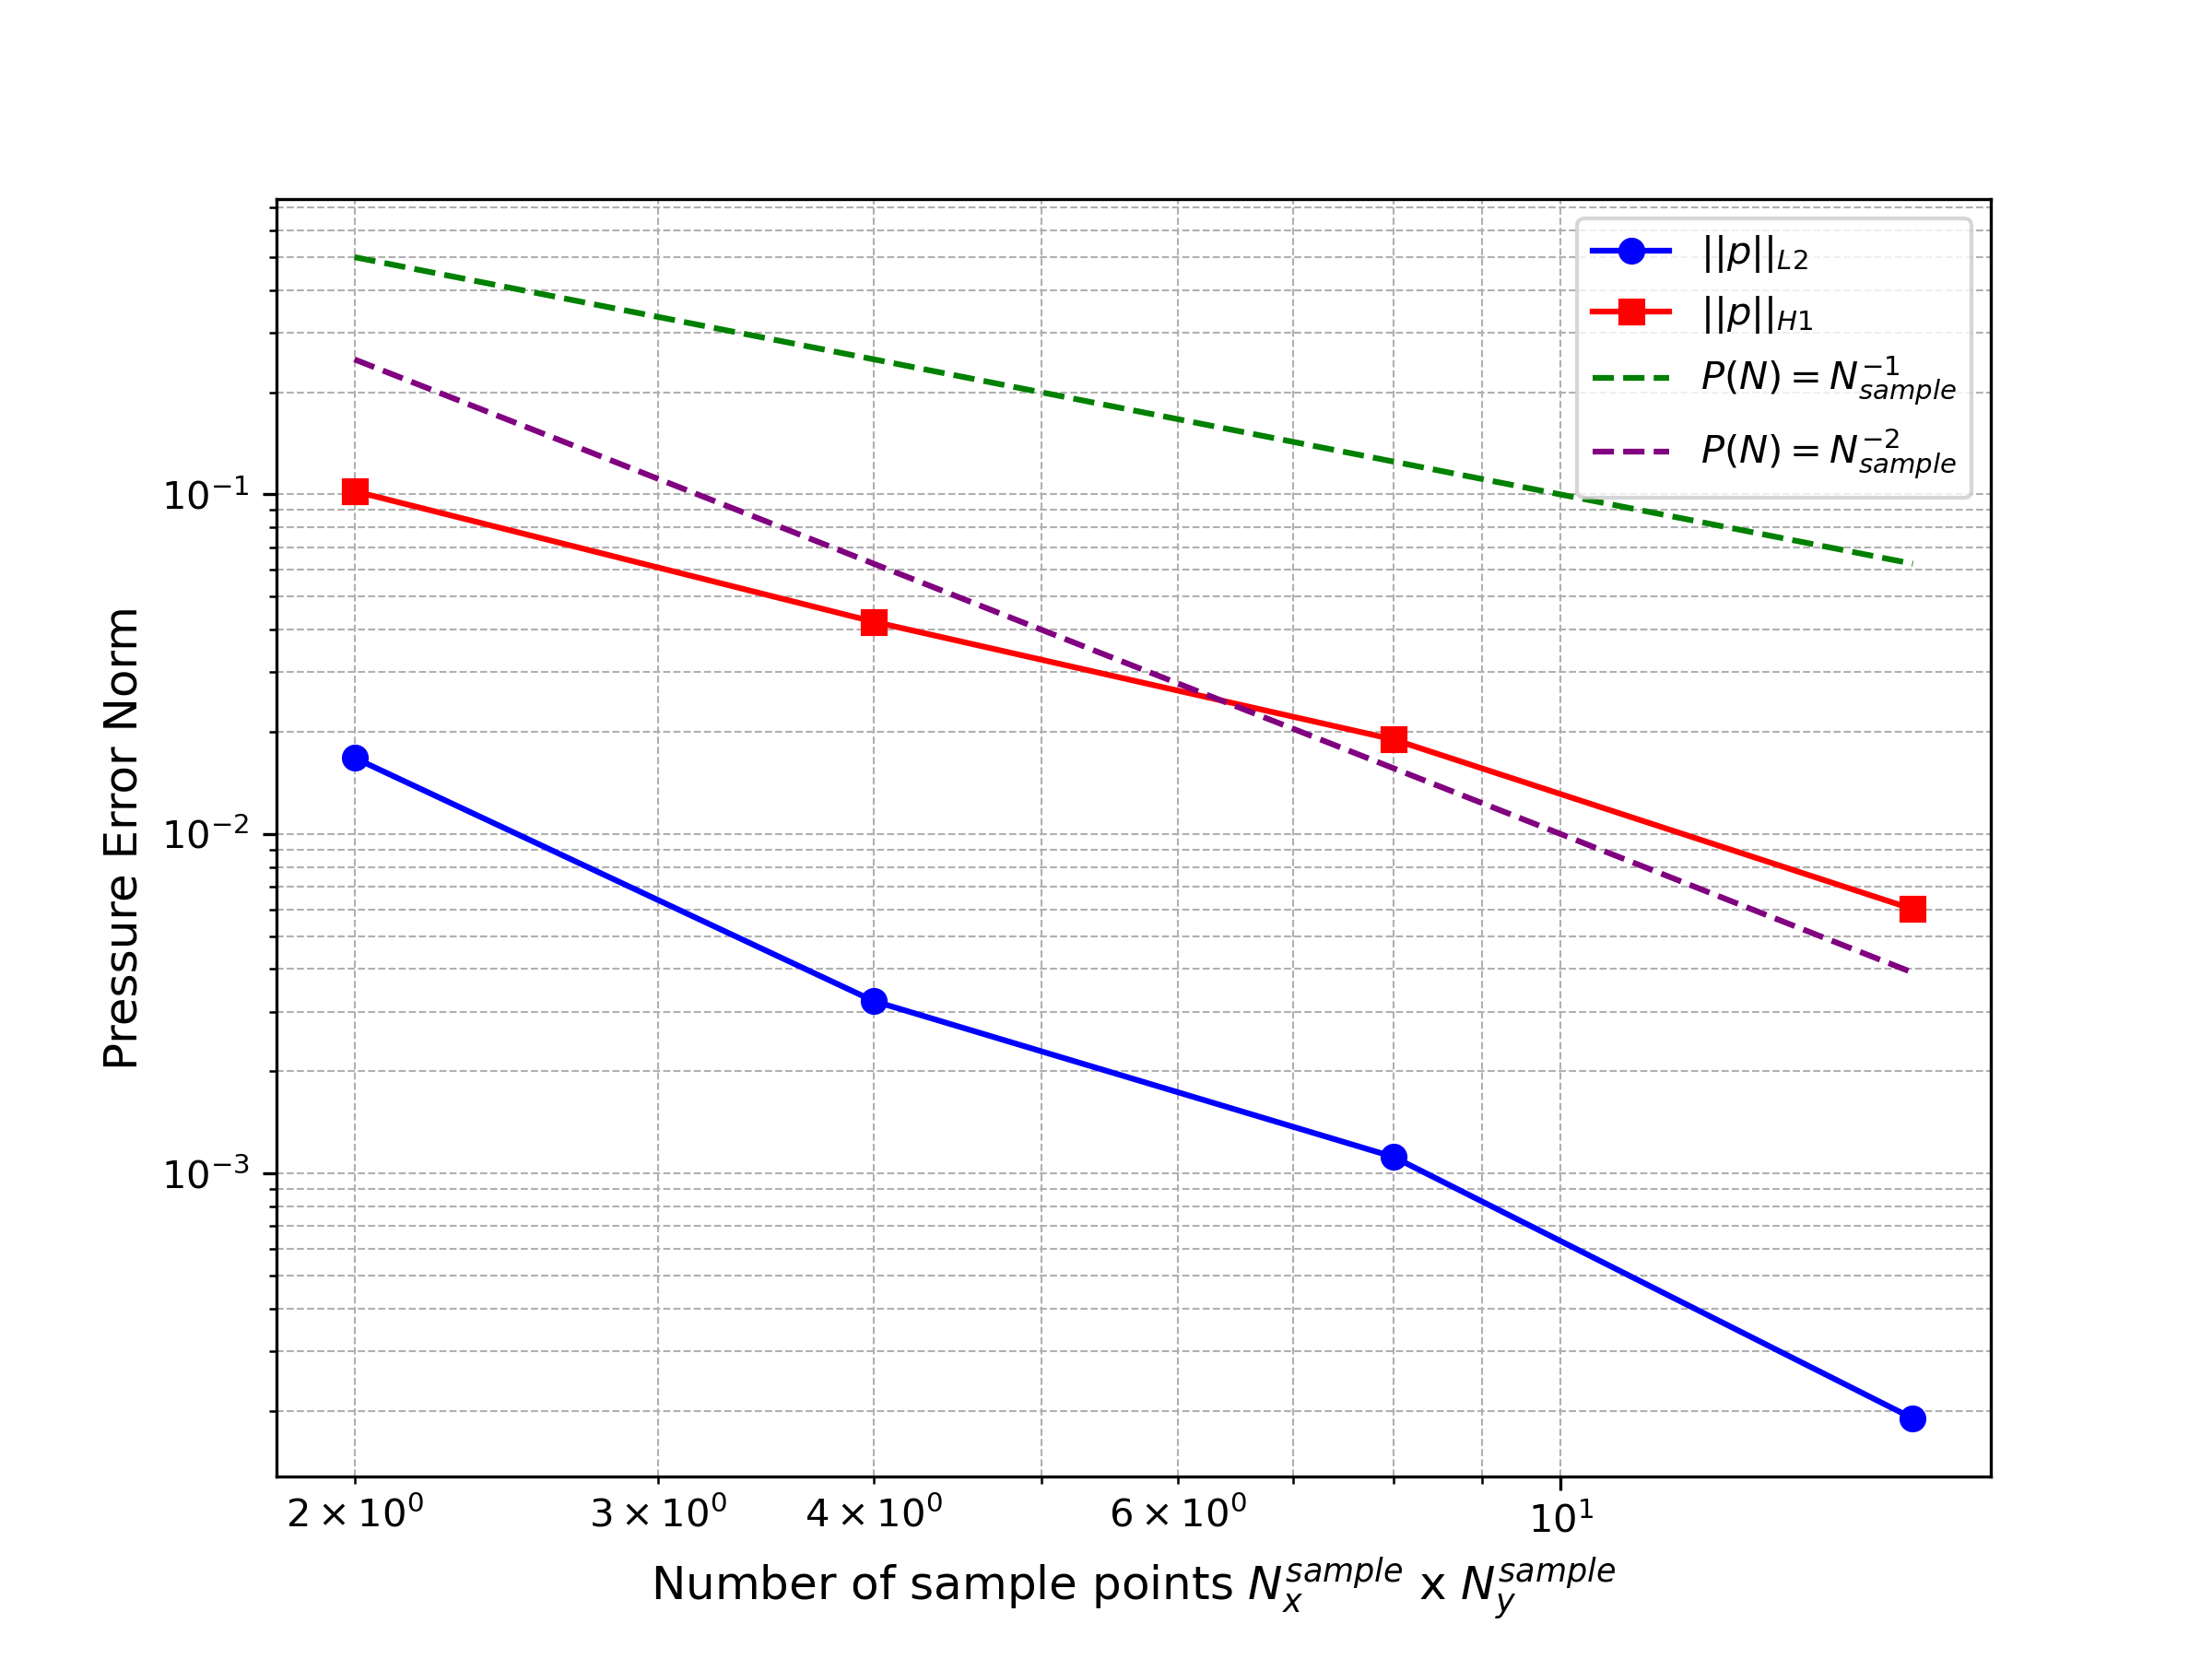
\includegraphics[width=\linewidth]{Figuras/Convergencia_amostras/pressure_convergence_Nsample_20_homogeneous_perm.png}
		\caption{Convergência de $p$ na norma $L^{2}$ e na norma $H^{1}$.}
		\label{fig:pressure_convergence_Nsample_20_homogeneous_perm}
	\end{subfigure}
	\begin{subfigure}[t]{0.45\linewidth}
		\centering
		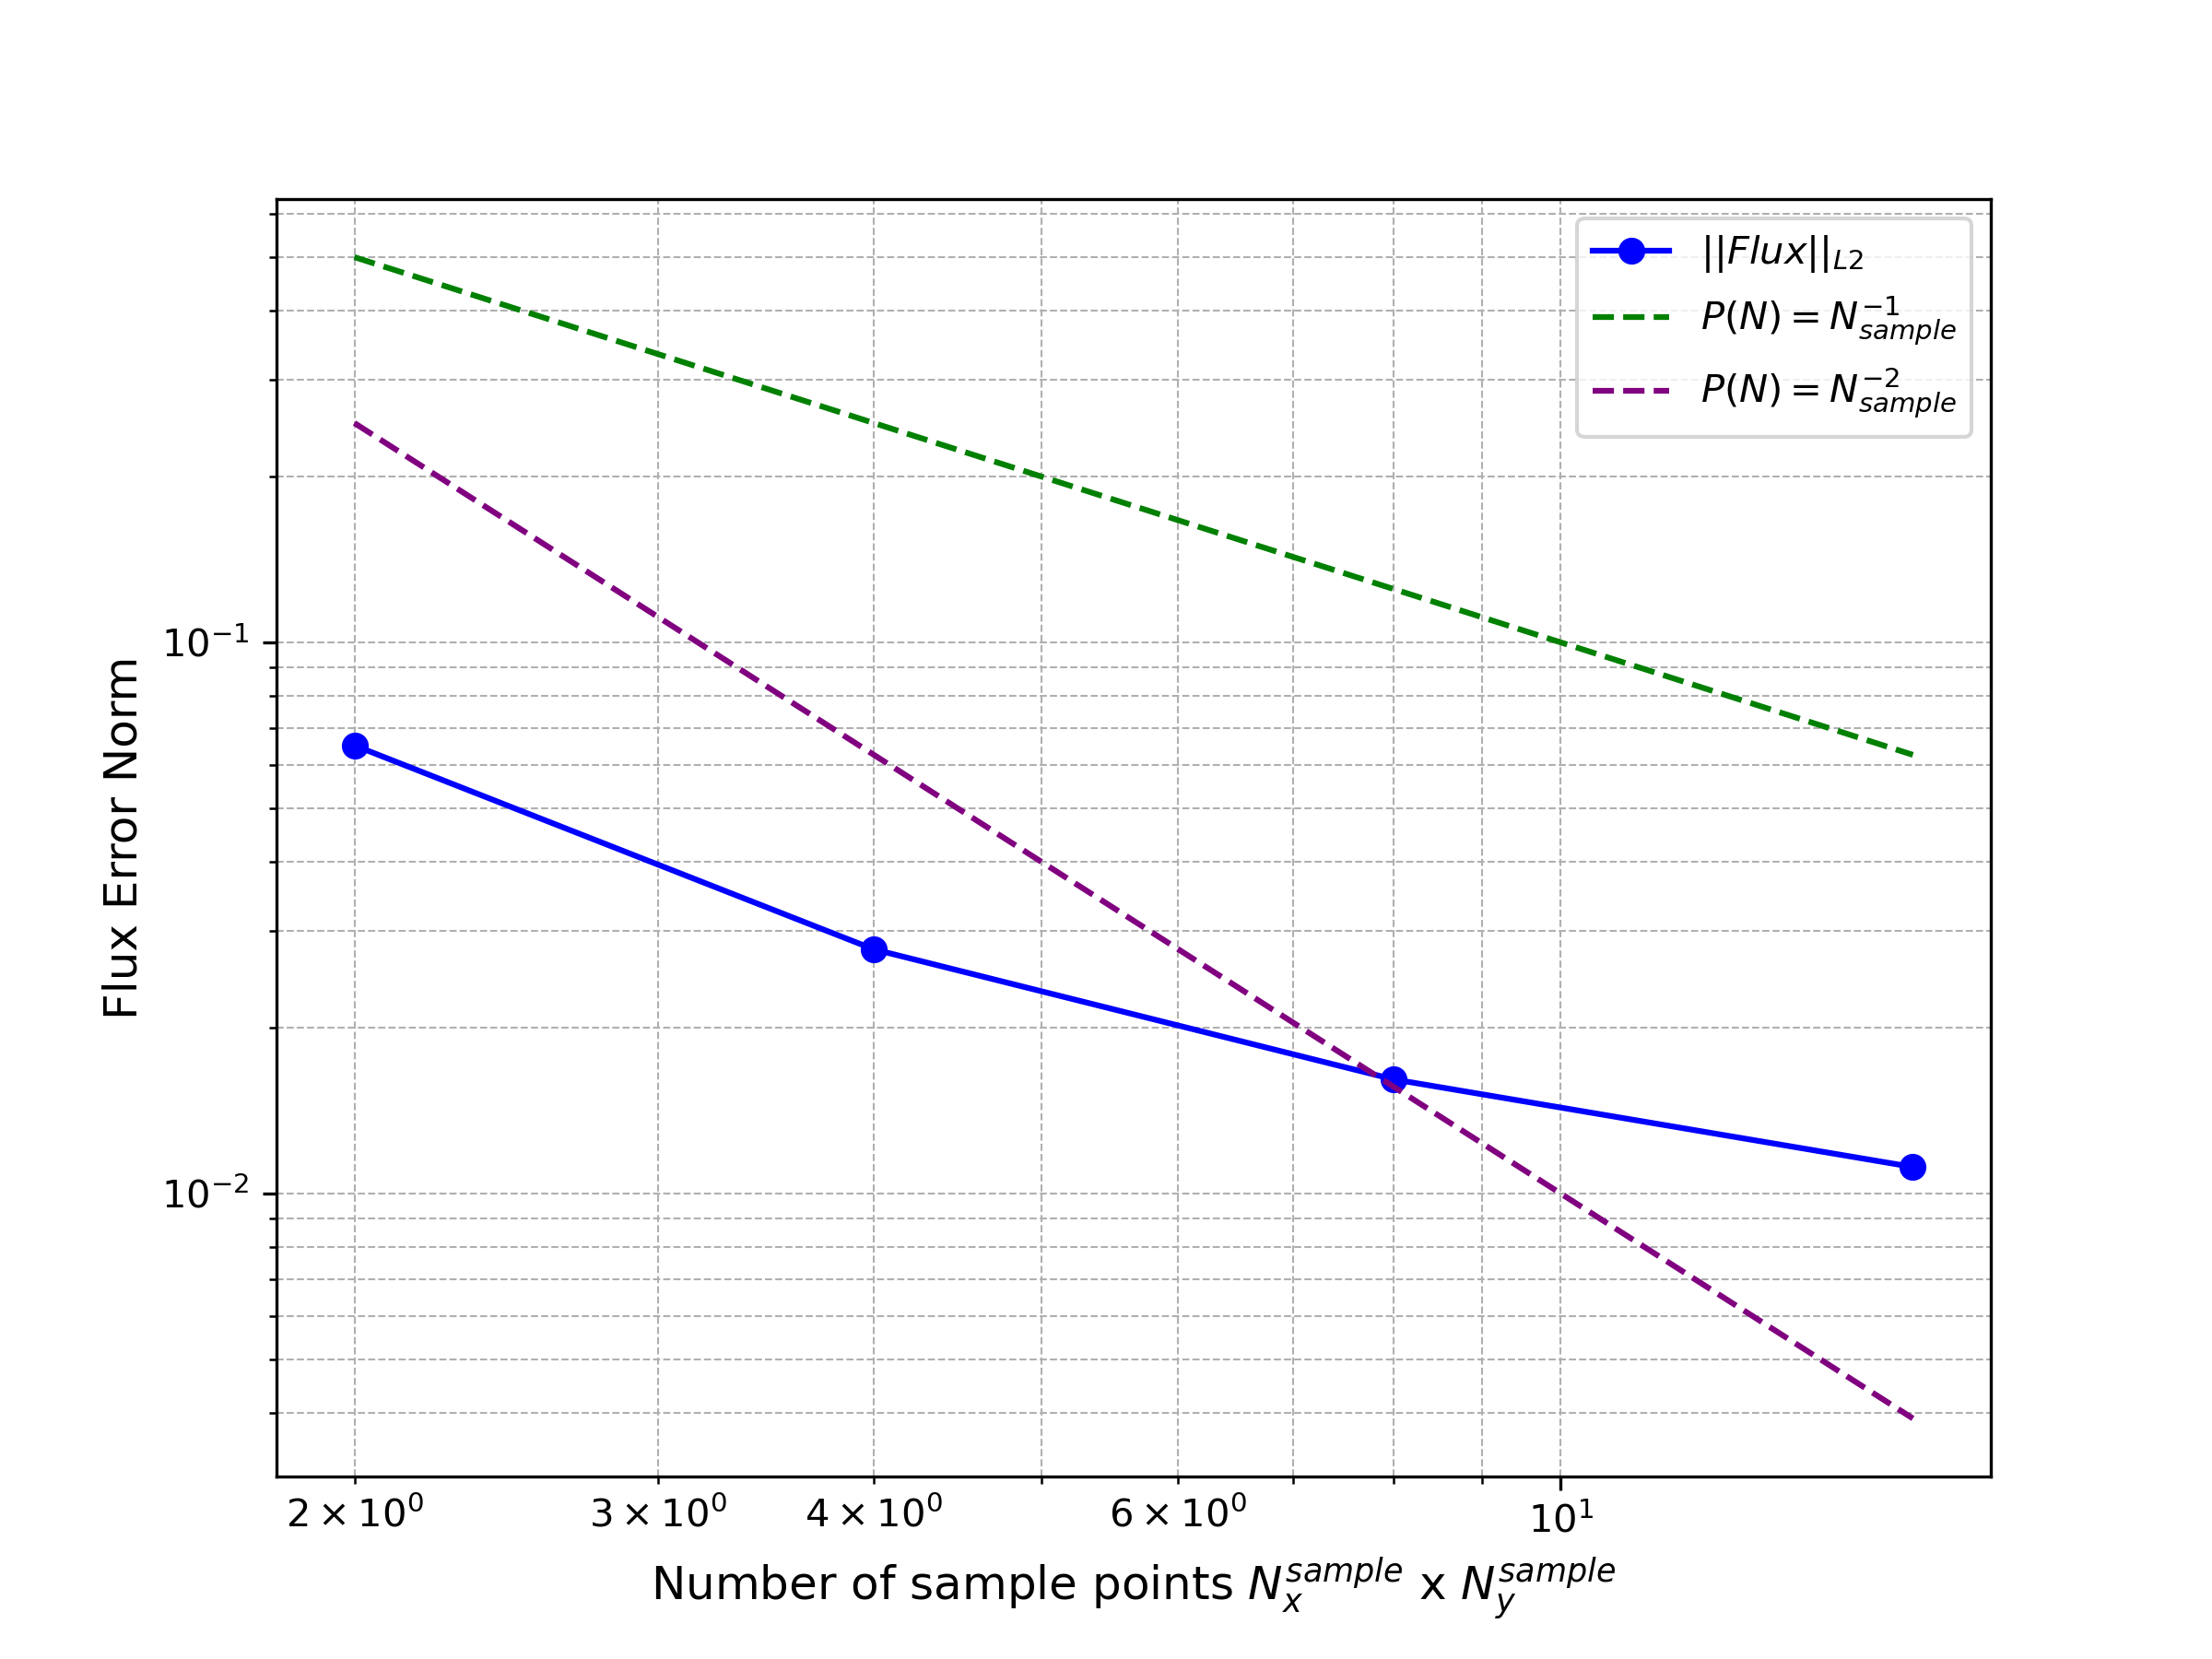
\includegraphics[width=\linewidth]{Figuras/Convergencia_amostras/flux_convergence_Nsample_20_homogeneous_perm.png}
		\caption{Convergência de $\mathbf{u}$ na norma $L^{2}$.}
		\label{fig:flux_convergence_Nsample_20_homogeneous_perm}
	\end{subfigure}
	\label{fig:convergence_coarse_mesh_homogeneous_perm}
\end{figure}

\begin{figure}[!ht]
	\centering
	\caption{Análise de convergência do campo escalar de pressões e do fluxo de Darcy em relação do número de pontos amostrais, em uma malha de elementos finitos $200 \times 200$ e um campo de permeabilidade homogêneo.}
	\begin{subfigure}[t]{0.45\linewidth}
		\centering
		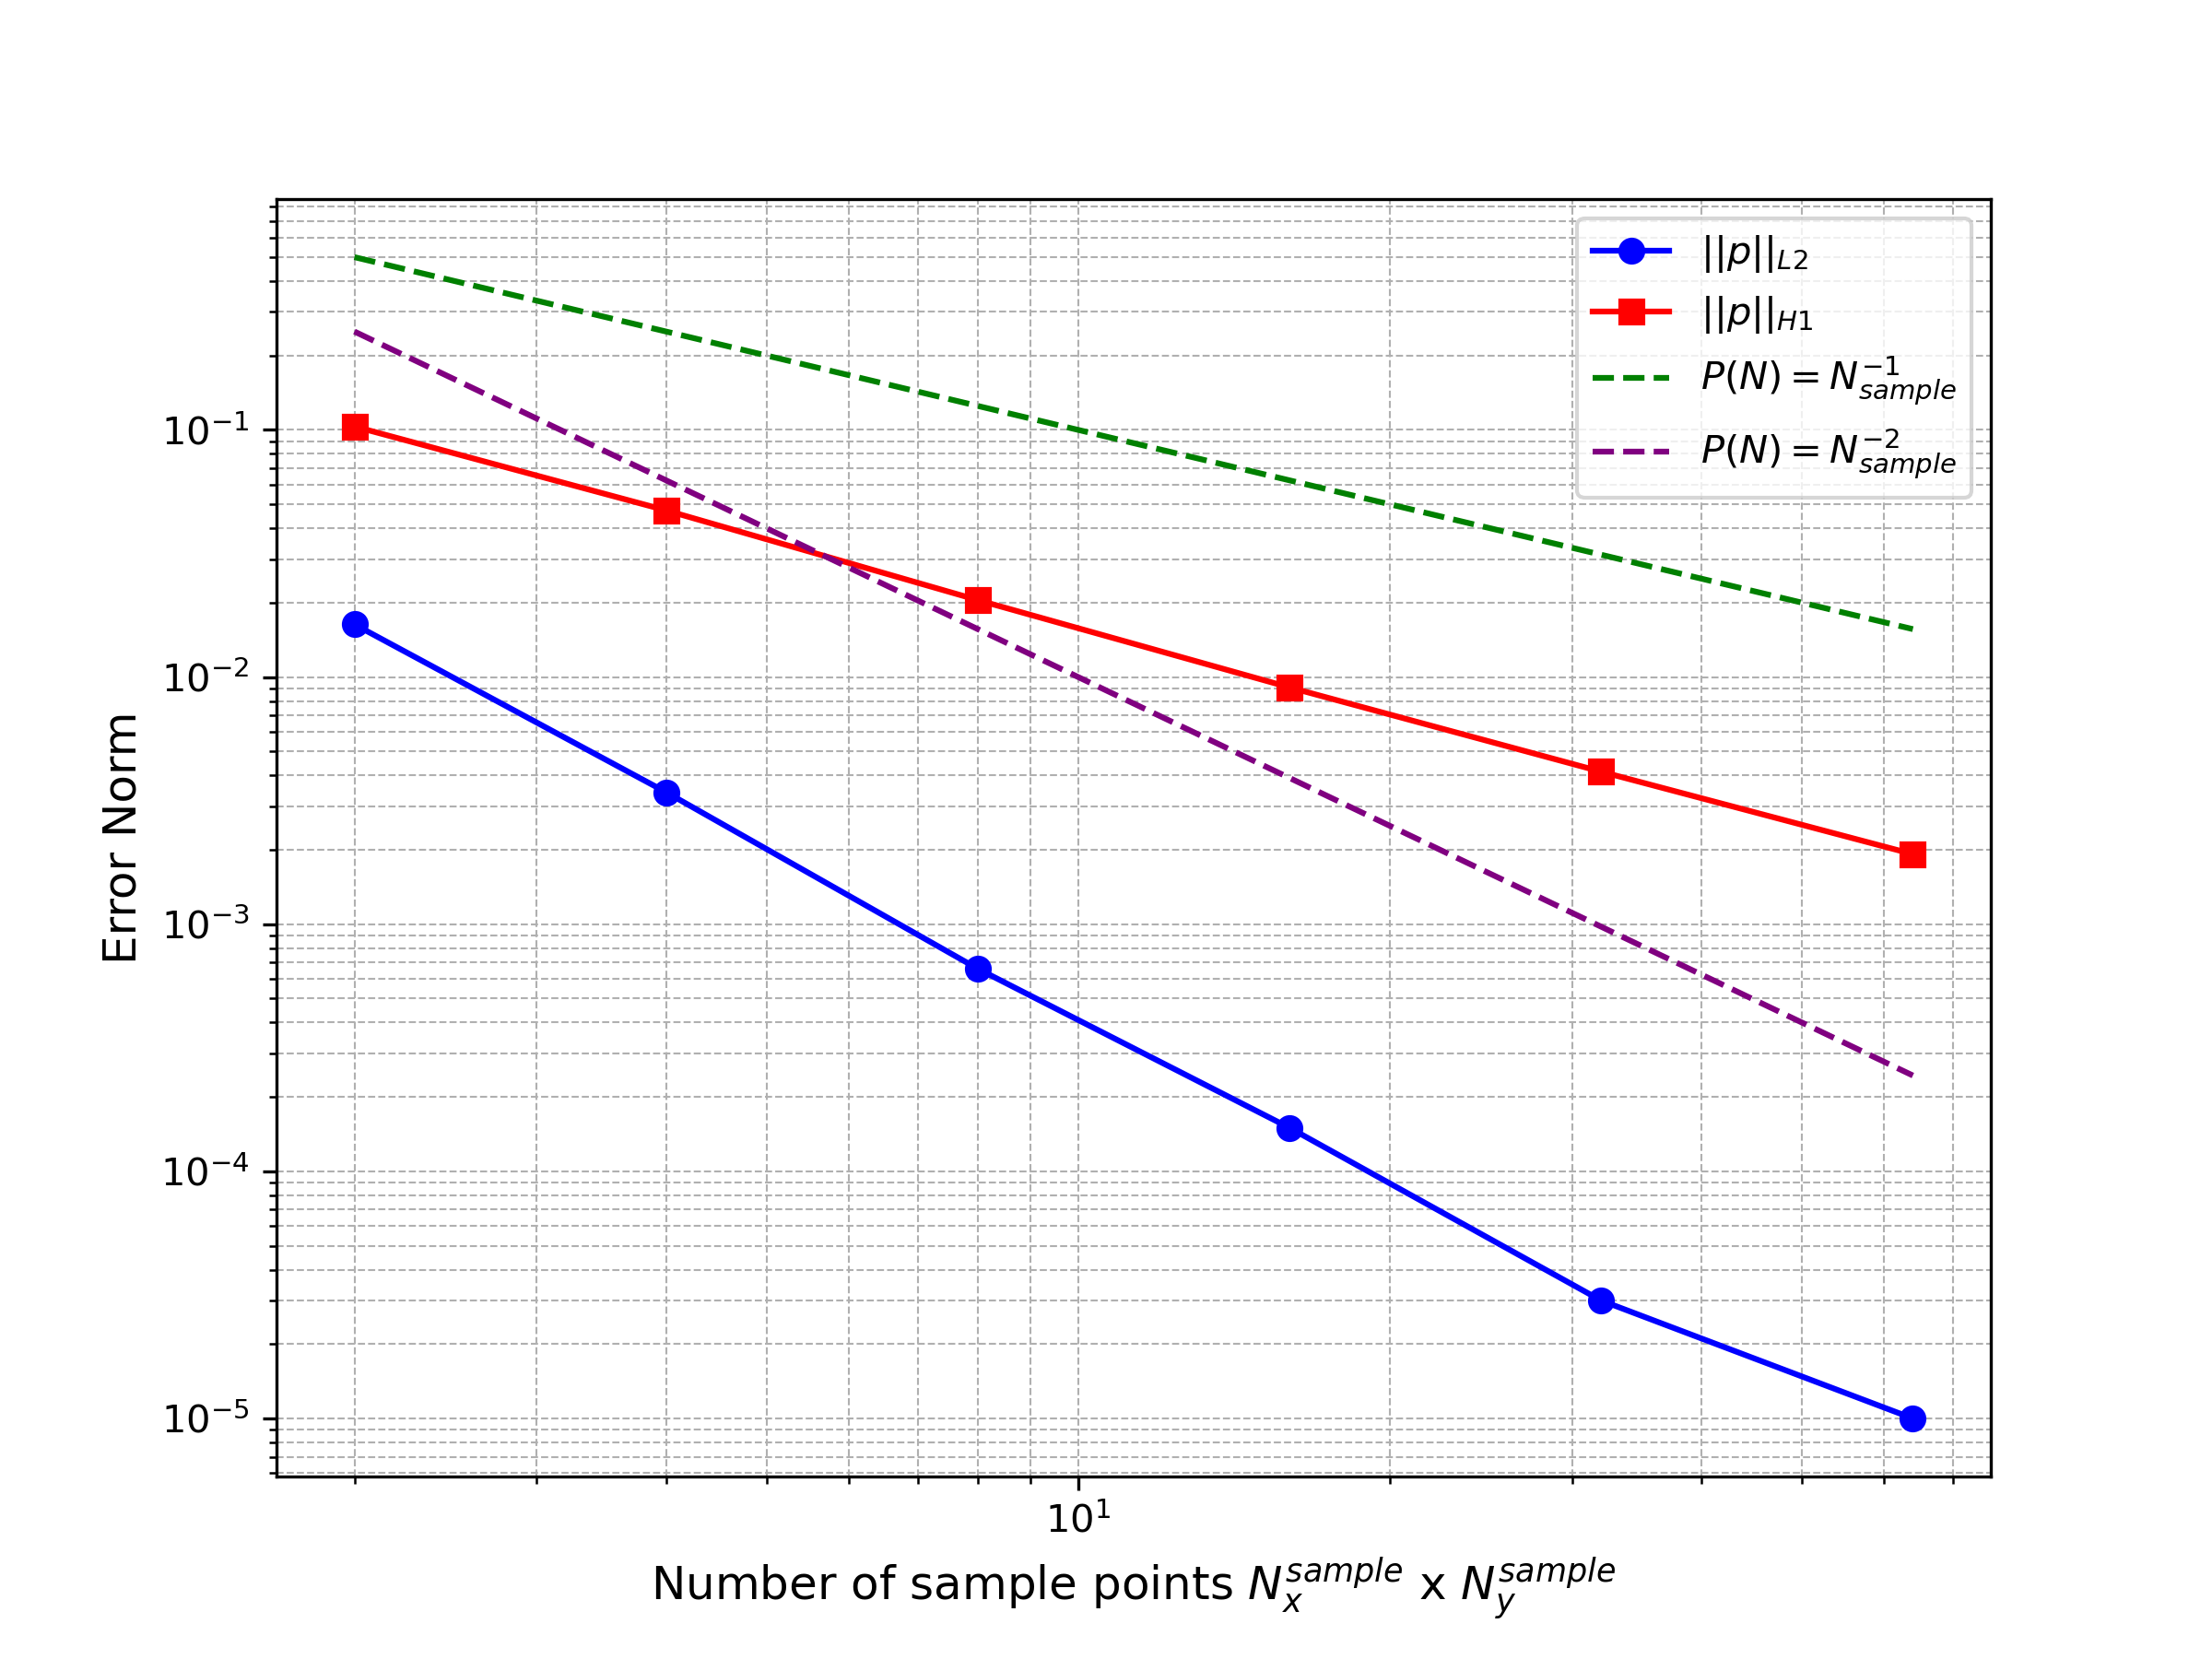
\includegraphics[width=\linewidth]{Figuras/Convergencia_amostras/pressure_convergence_Nsample_200_homogeneous_perm.png}
		\caption{Convergência de $p$ na norma $L^{2}$ e na norma $H^{1}$.}
		\label{fig:pressure_convergence_Nsample_200_homogeneous_perm}
	\end{subfigure}
	\begin{subfigure}[t]{0.45\linewidth}
		\centering
		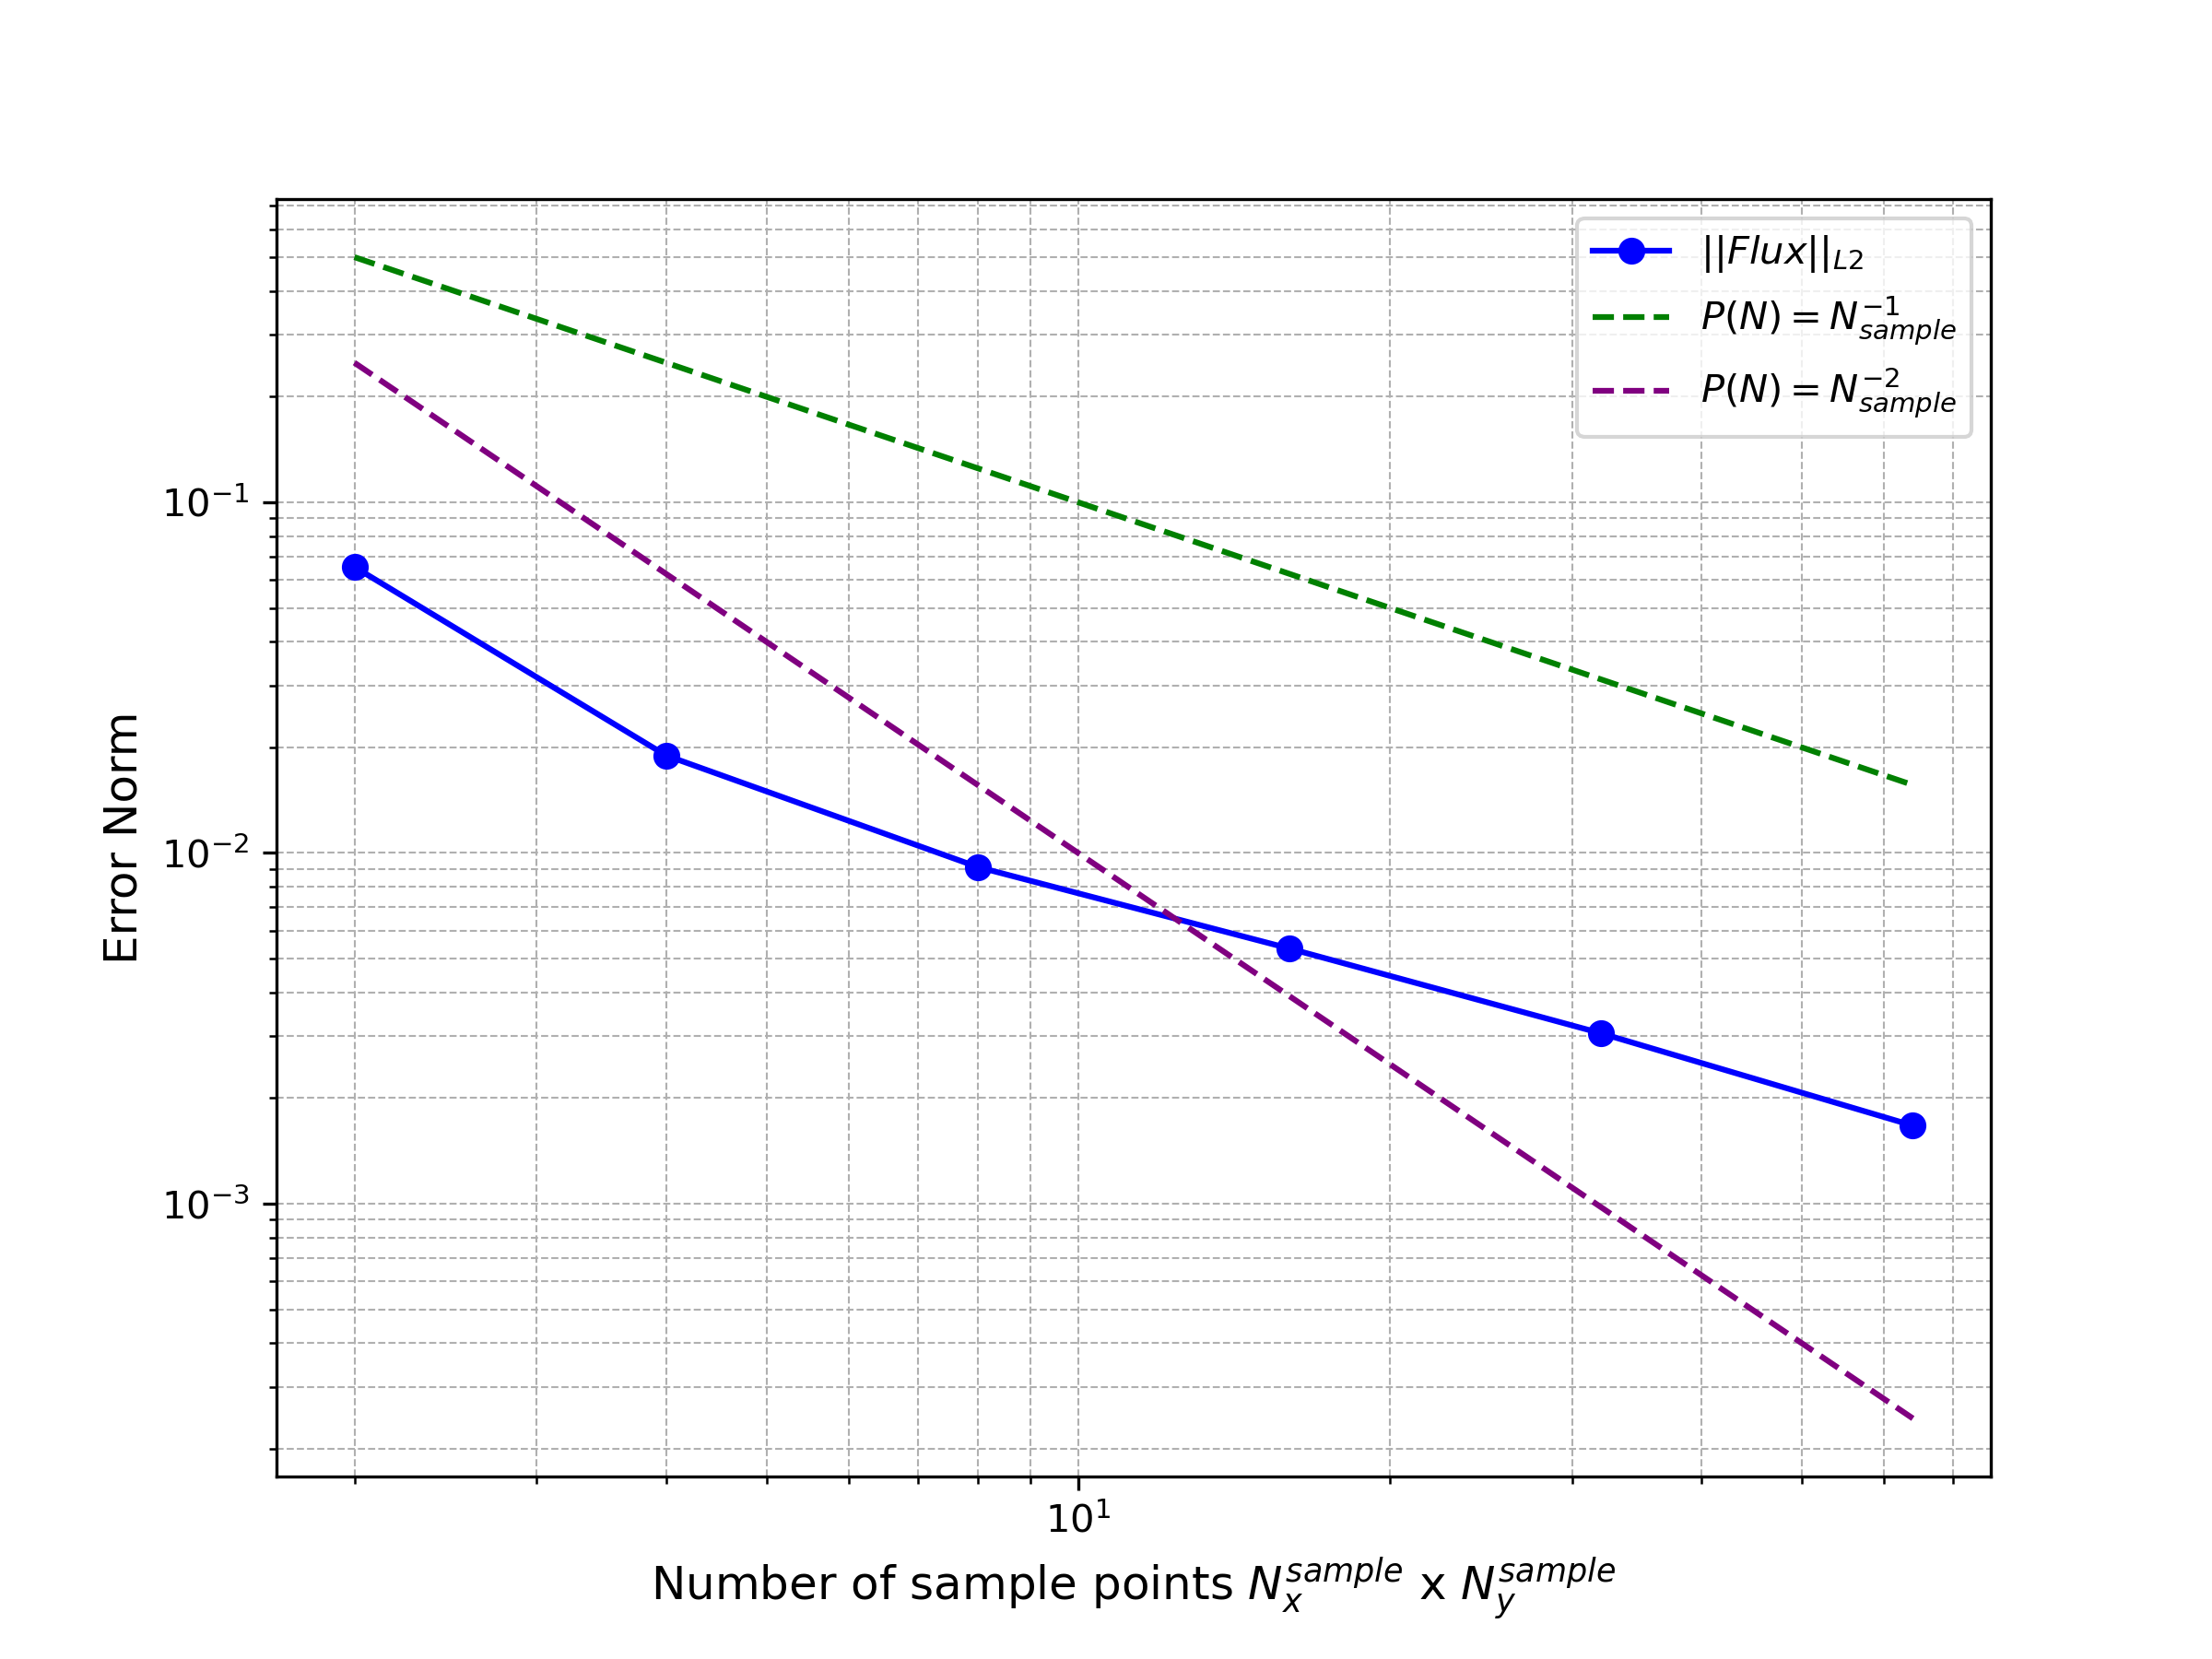
\includegraphics[width=\linewidth]{Figuras/Convergencia_amostras/flux_convergence_Nsample_200_homogeneous_perm.png}
		\caption{Convergência de $\mathbf{u}$ na norma $L^{2}$.}
		\label{fig:flux_convergence_Nsample_200_homogeneous_perm}
	\end{subfigure}
	\label{fig:convergence_fine_mesh_homogeneous_perm}
\end{figure}

\subsubsection{Permeabilidade heterogênea: função gaussiana}

\begin{equation}
	K(x,y) = K_{0} + e^{-A\big(x-\frac{L}{2}\big)^{2} + \big(y-\frac{L}{2}\big)^{2}}, \quad \begin{cases}
		K_{0} = 0.01 \\
		A = 10
	\end{cases}
\end{equation}

\begin{figure}[!ht]
	\centering
	\caption{Ilustração do(s): (a) pontos amostrais no espaço de fases ($\sigma \times \partial_{x} u$), (b) campo escalar de pressões, $p$, (c) multiplicadores de Lagrange, $\lambda$ e (d) fluxo de Darcy, $\mathbf{u}$ para o caso de permeabilidade heterogênea.}
	\begin{subfigure}[t]{0.45\linewidth}
		\centering
		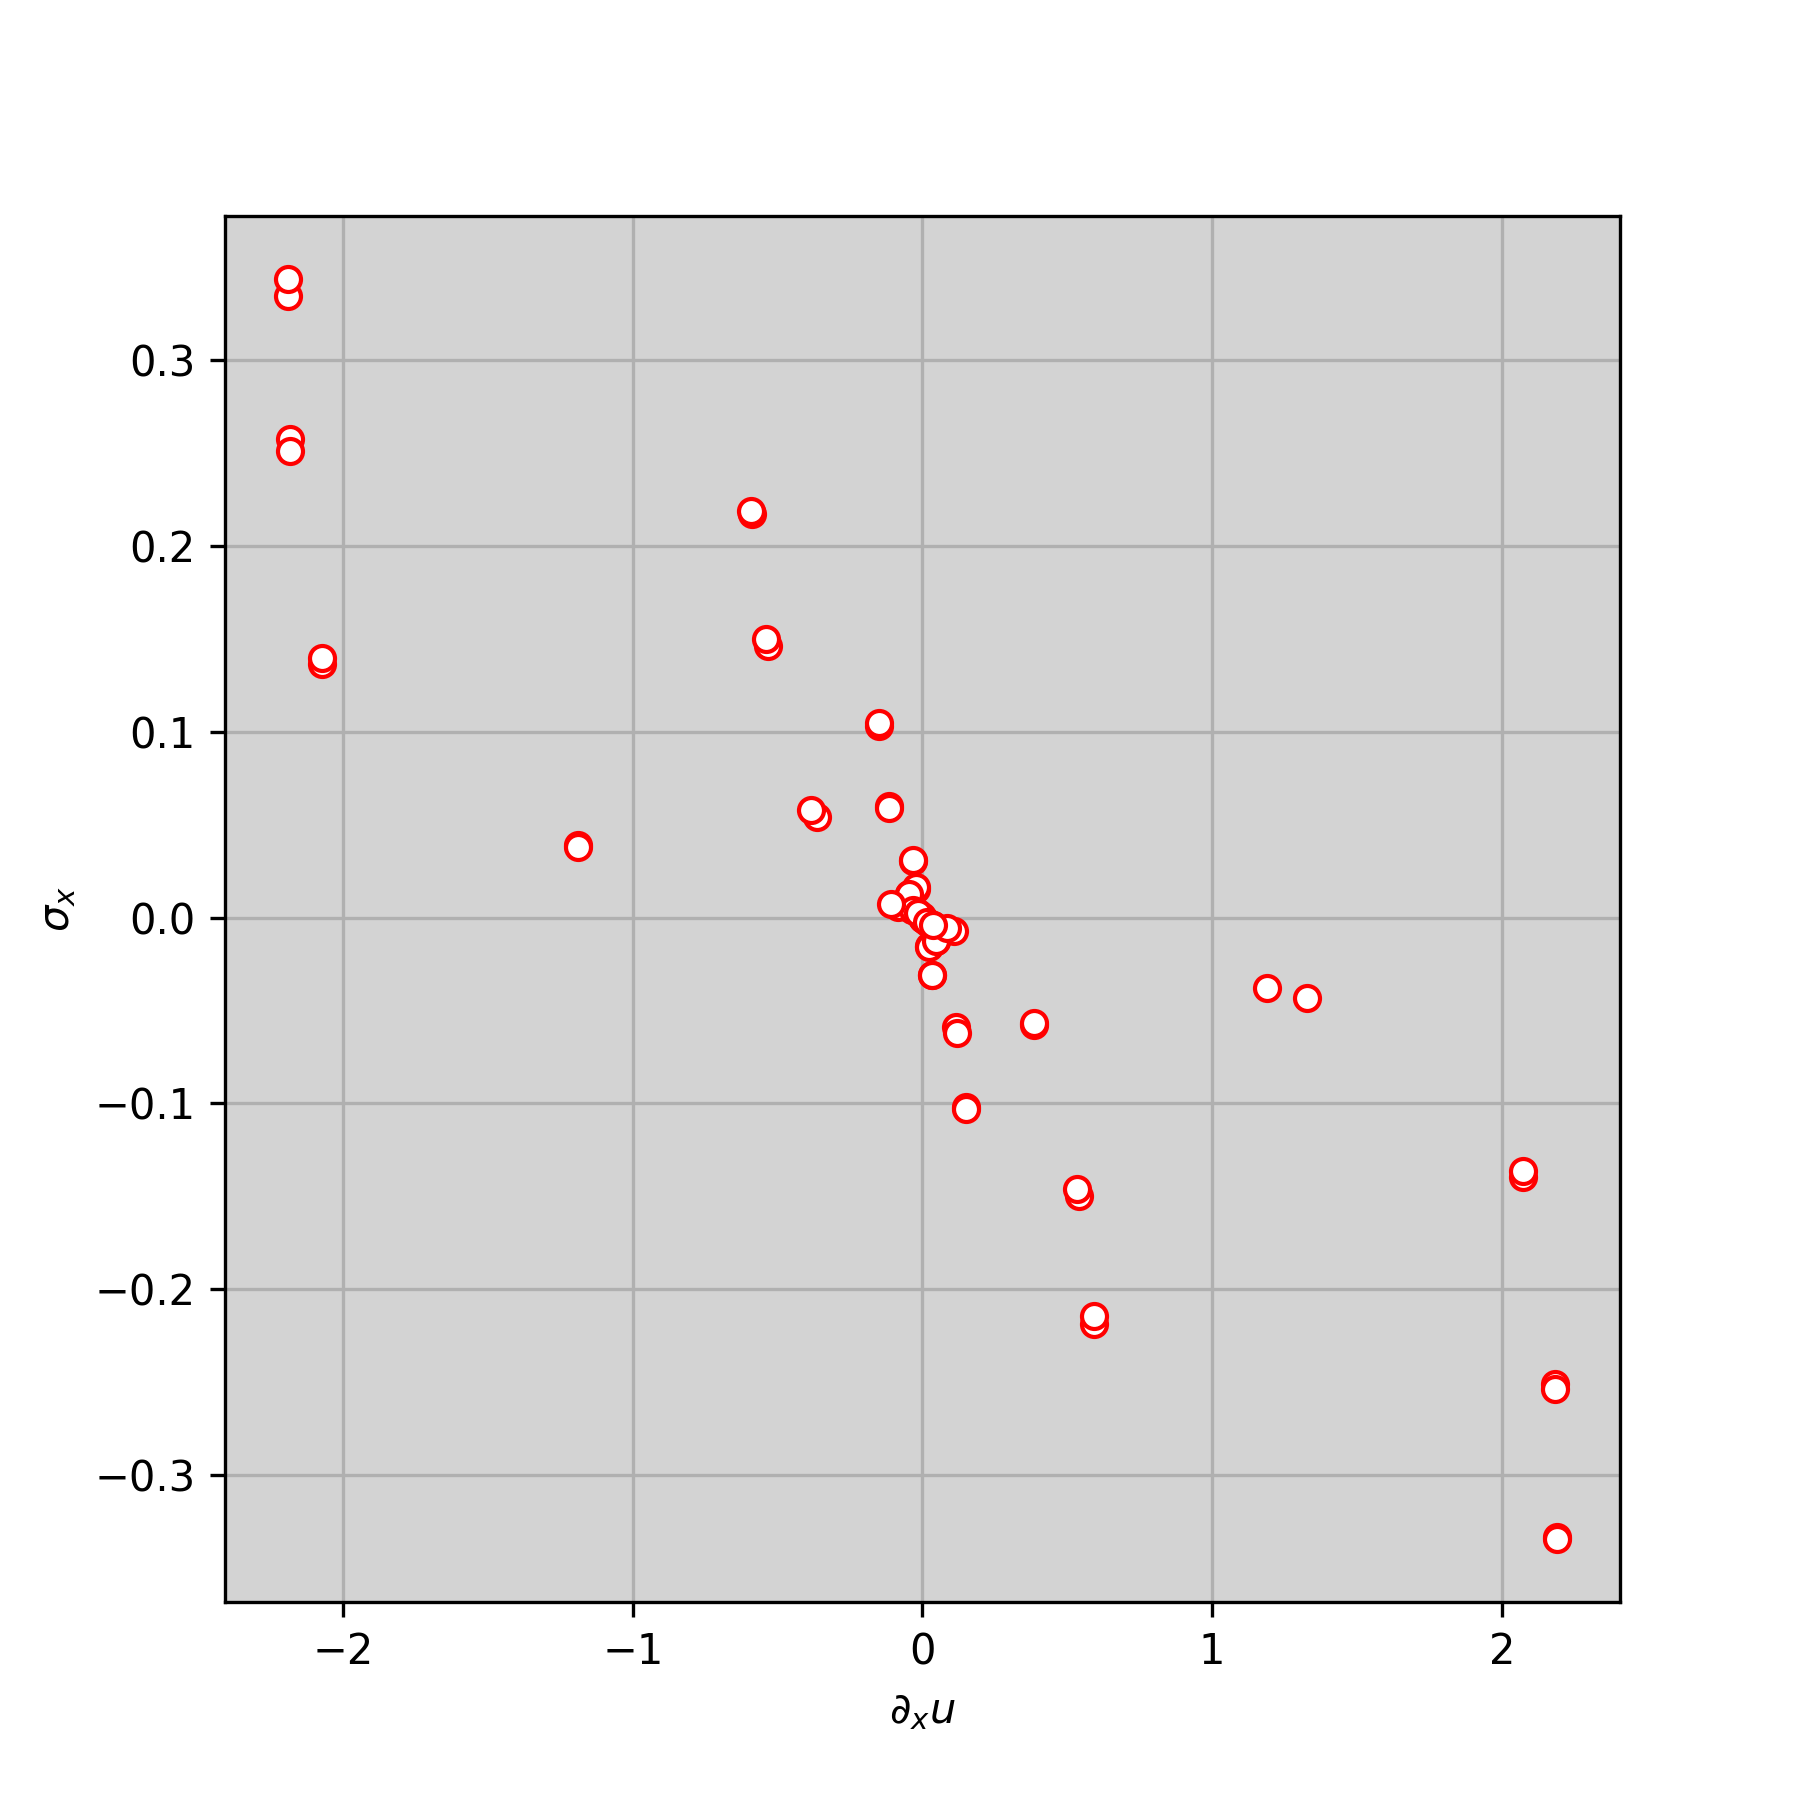
\includegraphics[width=0.94\linewidth]{Figuras/Convergencia_amostras/N_sample_8_gaussian.png}
		\caption{Número de pontos amostrais no espaço de fases ($\sigma \times \partial_{x} u$).}
		\label{fig:N_sample_8_gaussian}
	\end{subfigure}
	\begin{subfigure}[t]{0.45\linewidth}
		\centering
		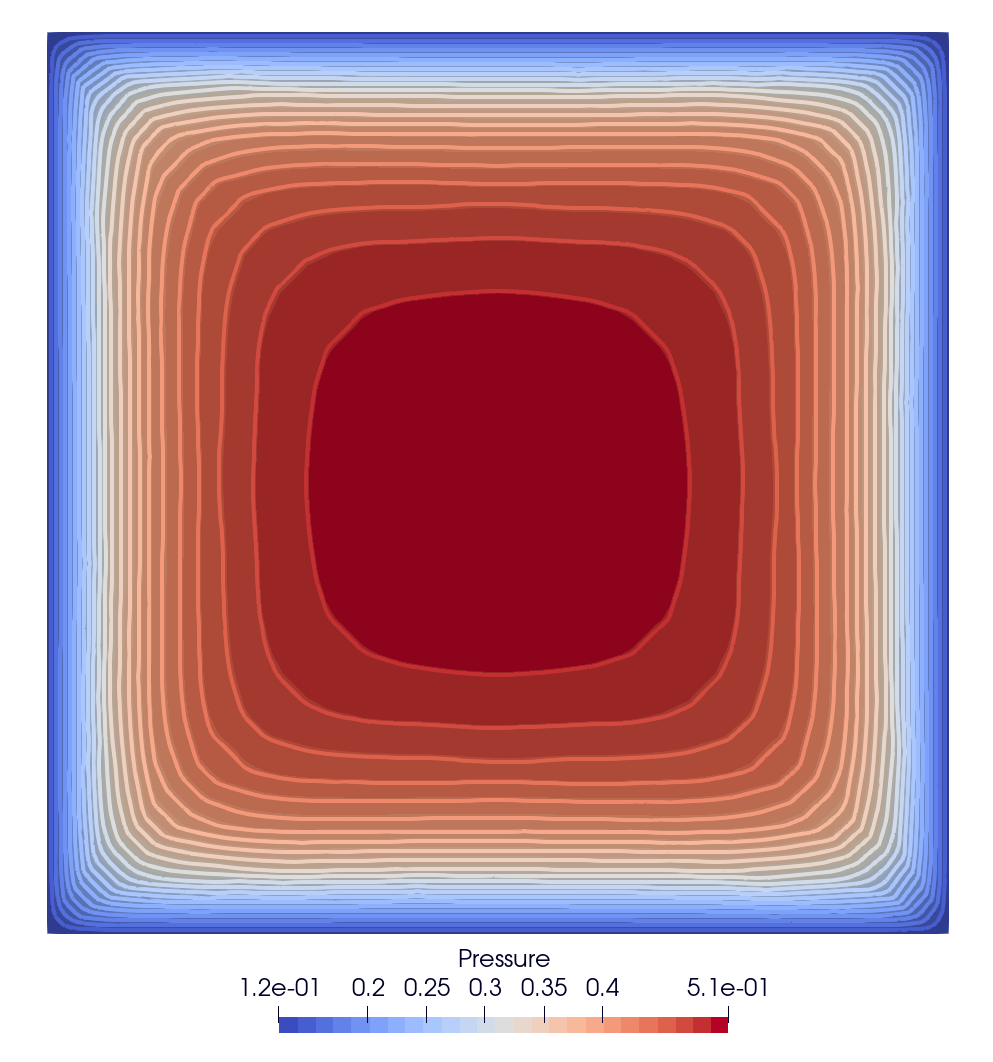
\includegraphics[width=0.8\linewidth]{Figuras/Convergencia_amostras/pressure_gaussian_perm.png}
		\caption{Campo escalar de pressão, $p$.}
		\label{fig:pressure_gaussian_perm}
	\end{subfigure}
	\begin{subfigure}[t]{0.45\linewidth}
		\centering
		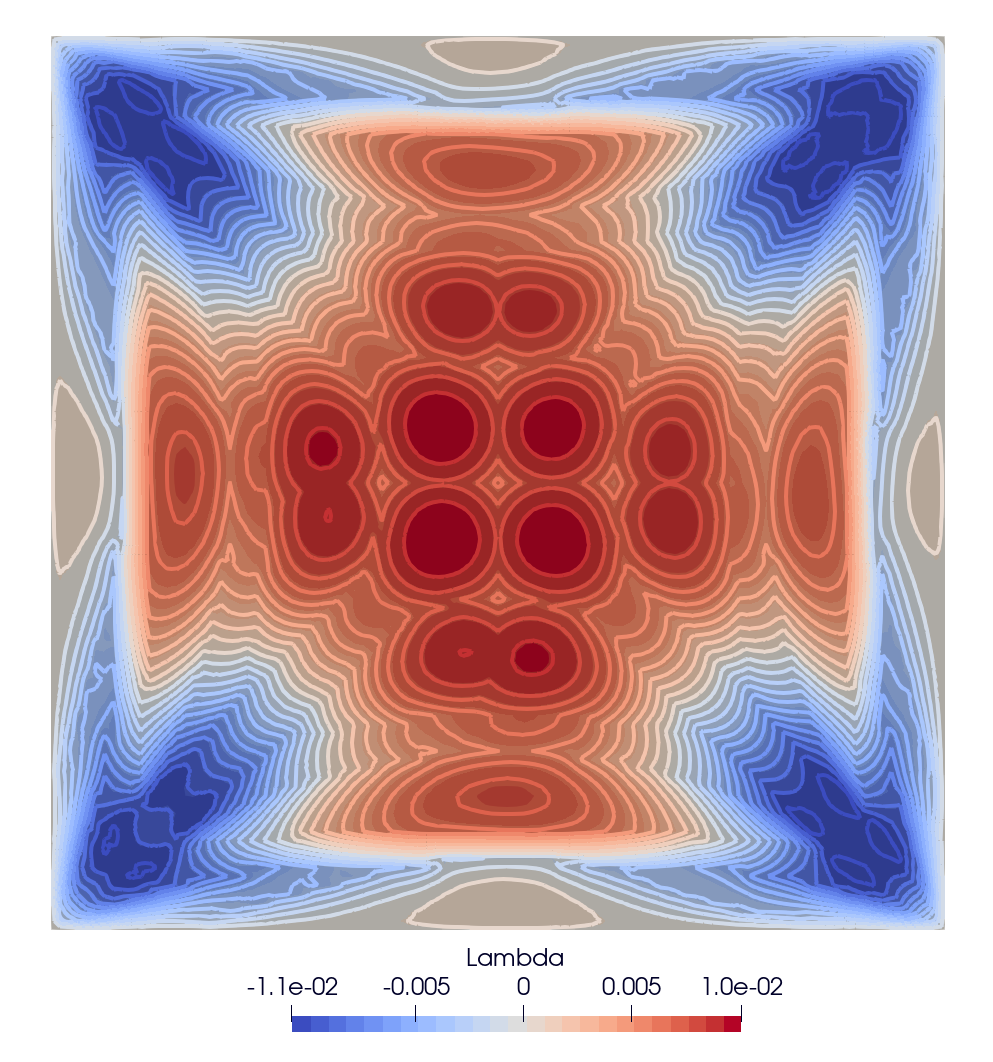
\includegraphics[width=0.8\linewidth]{Figuras/Convergencia_amostras/lambda_gaussian_perm.png}
		\caption{Multiplicadores de Lagrange, $\lambda$.}
		\label{fig:lambda_gaussian_perm}
	\end{subfigure}
	\begin{subfigure}[t]{0.45\linewidth}
		\centering
		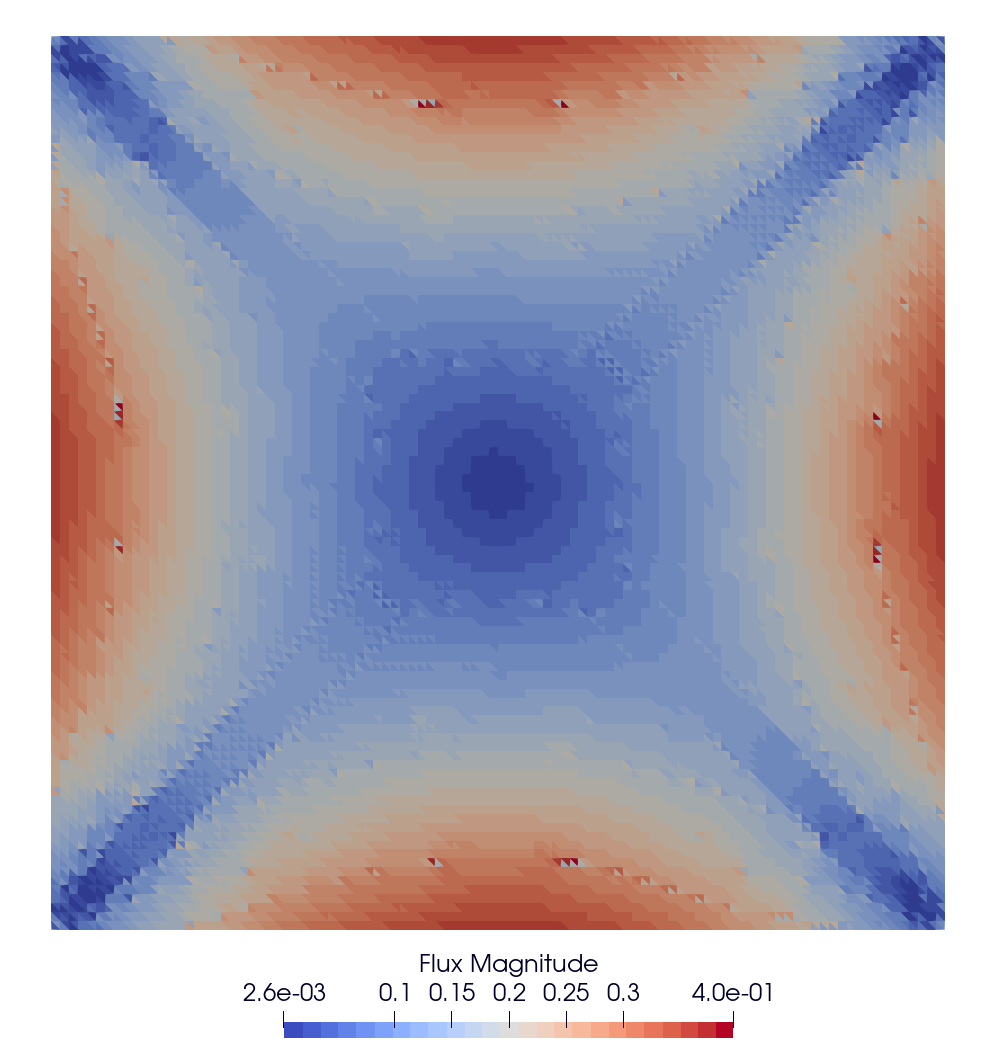
\includegraphics[width=0.8\linewidth]{Figuras/Convergencia_amostras/flux_gaussian_perm.png}
		\caption{Fluxo de Darcy, $\mathbf{u}$.}
		\label{fig:flux_gaussian_perm}
	\end{subfigure}
	\label{fig:graphs_heterogeneous_perm}
\end{figure}


\begin{figure}[!ht]
	\centering
	\caption{Análise de convergência do campo escalar de pressões e do fluxo de Darcy em relação do número de pontos amostrais, em uma malha de elementos finitos $20 \times 20$ e um campo de permeabilidade heterogêneo.}
	\begin{subfigure}[t]{0.45\linewidth}
		\centering
		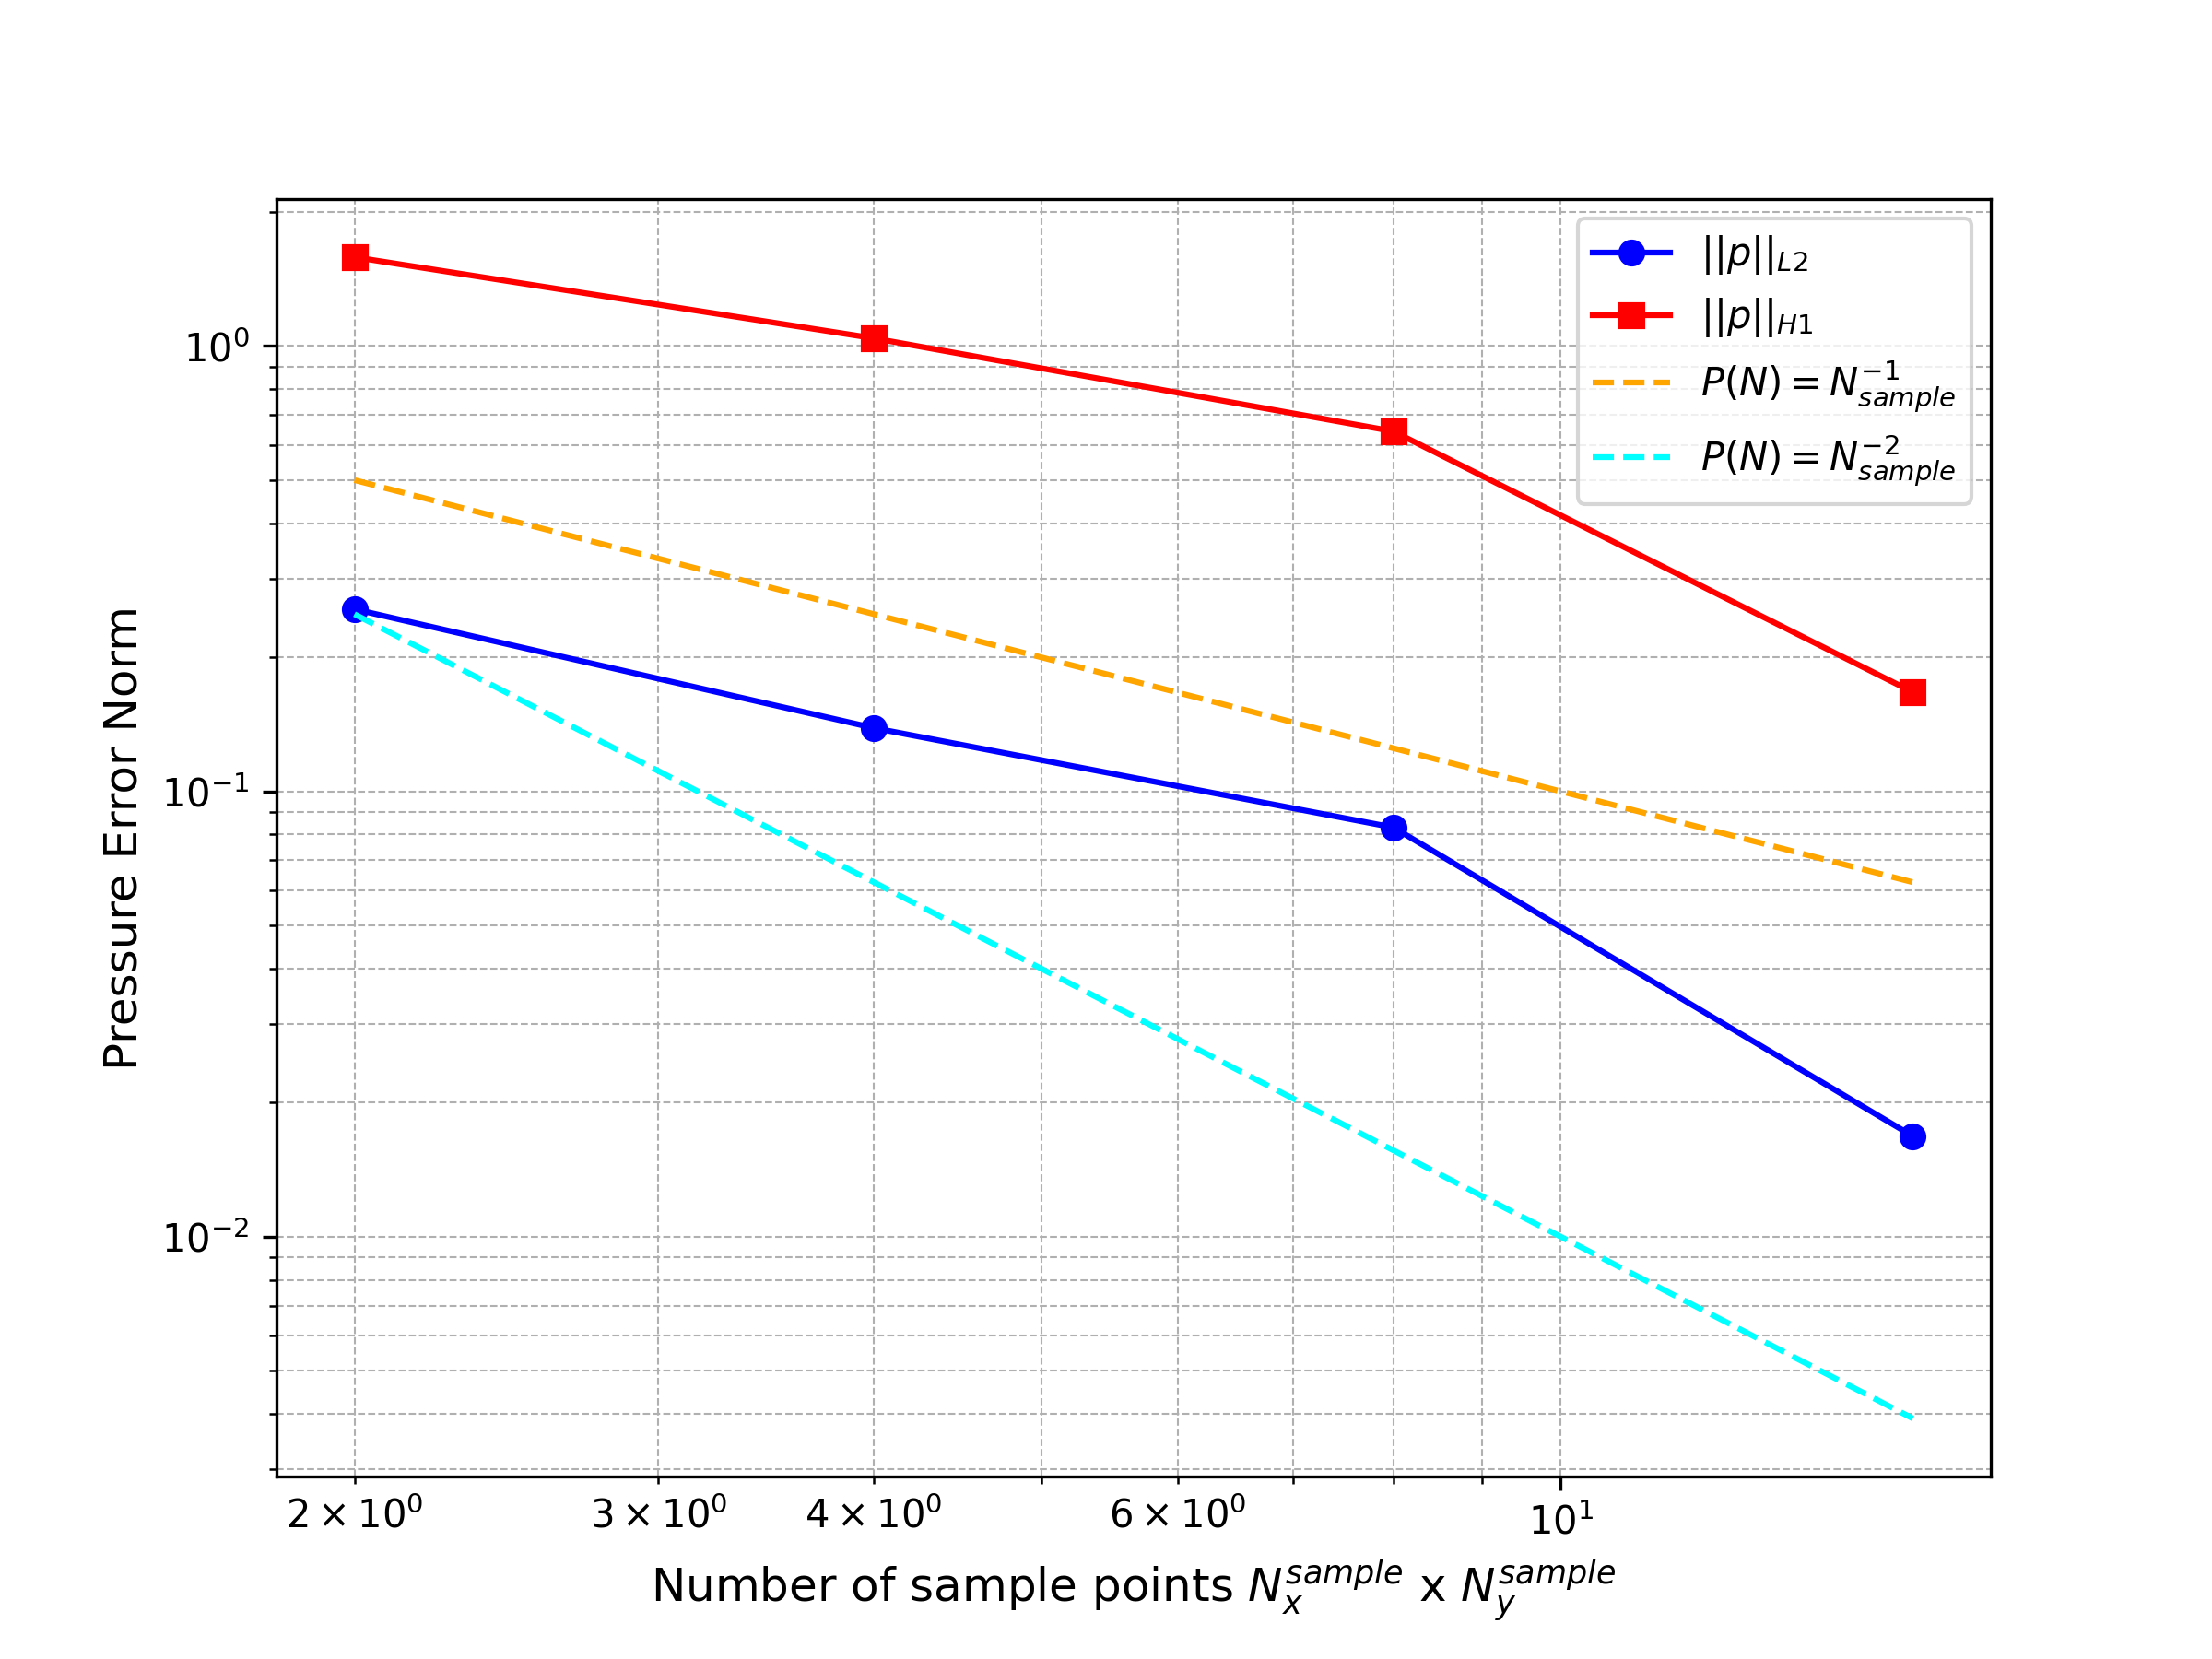
\includegraphics[width=\linewidth]{Figuras/Convergencia_amostras/pressure_convergence_Nsample_20_heterogeneous_perm.png}
		\caption{Convergência de $p$ na norma $L^{2}$ e na norma $H^{1}$.}
		\label{fig:pressure_convergence_Nsample_20_heterogeneous_perm}
	\end{subfigure}
	\begin{subfigure}[t]{0.45\linewidth}
		\centering
		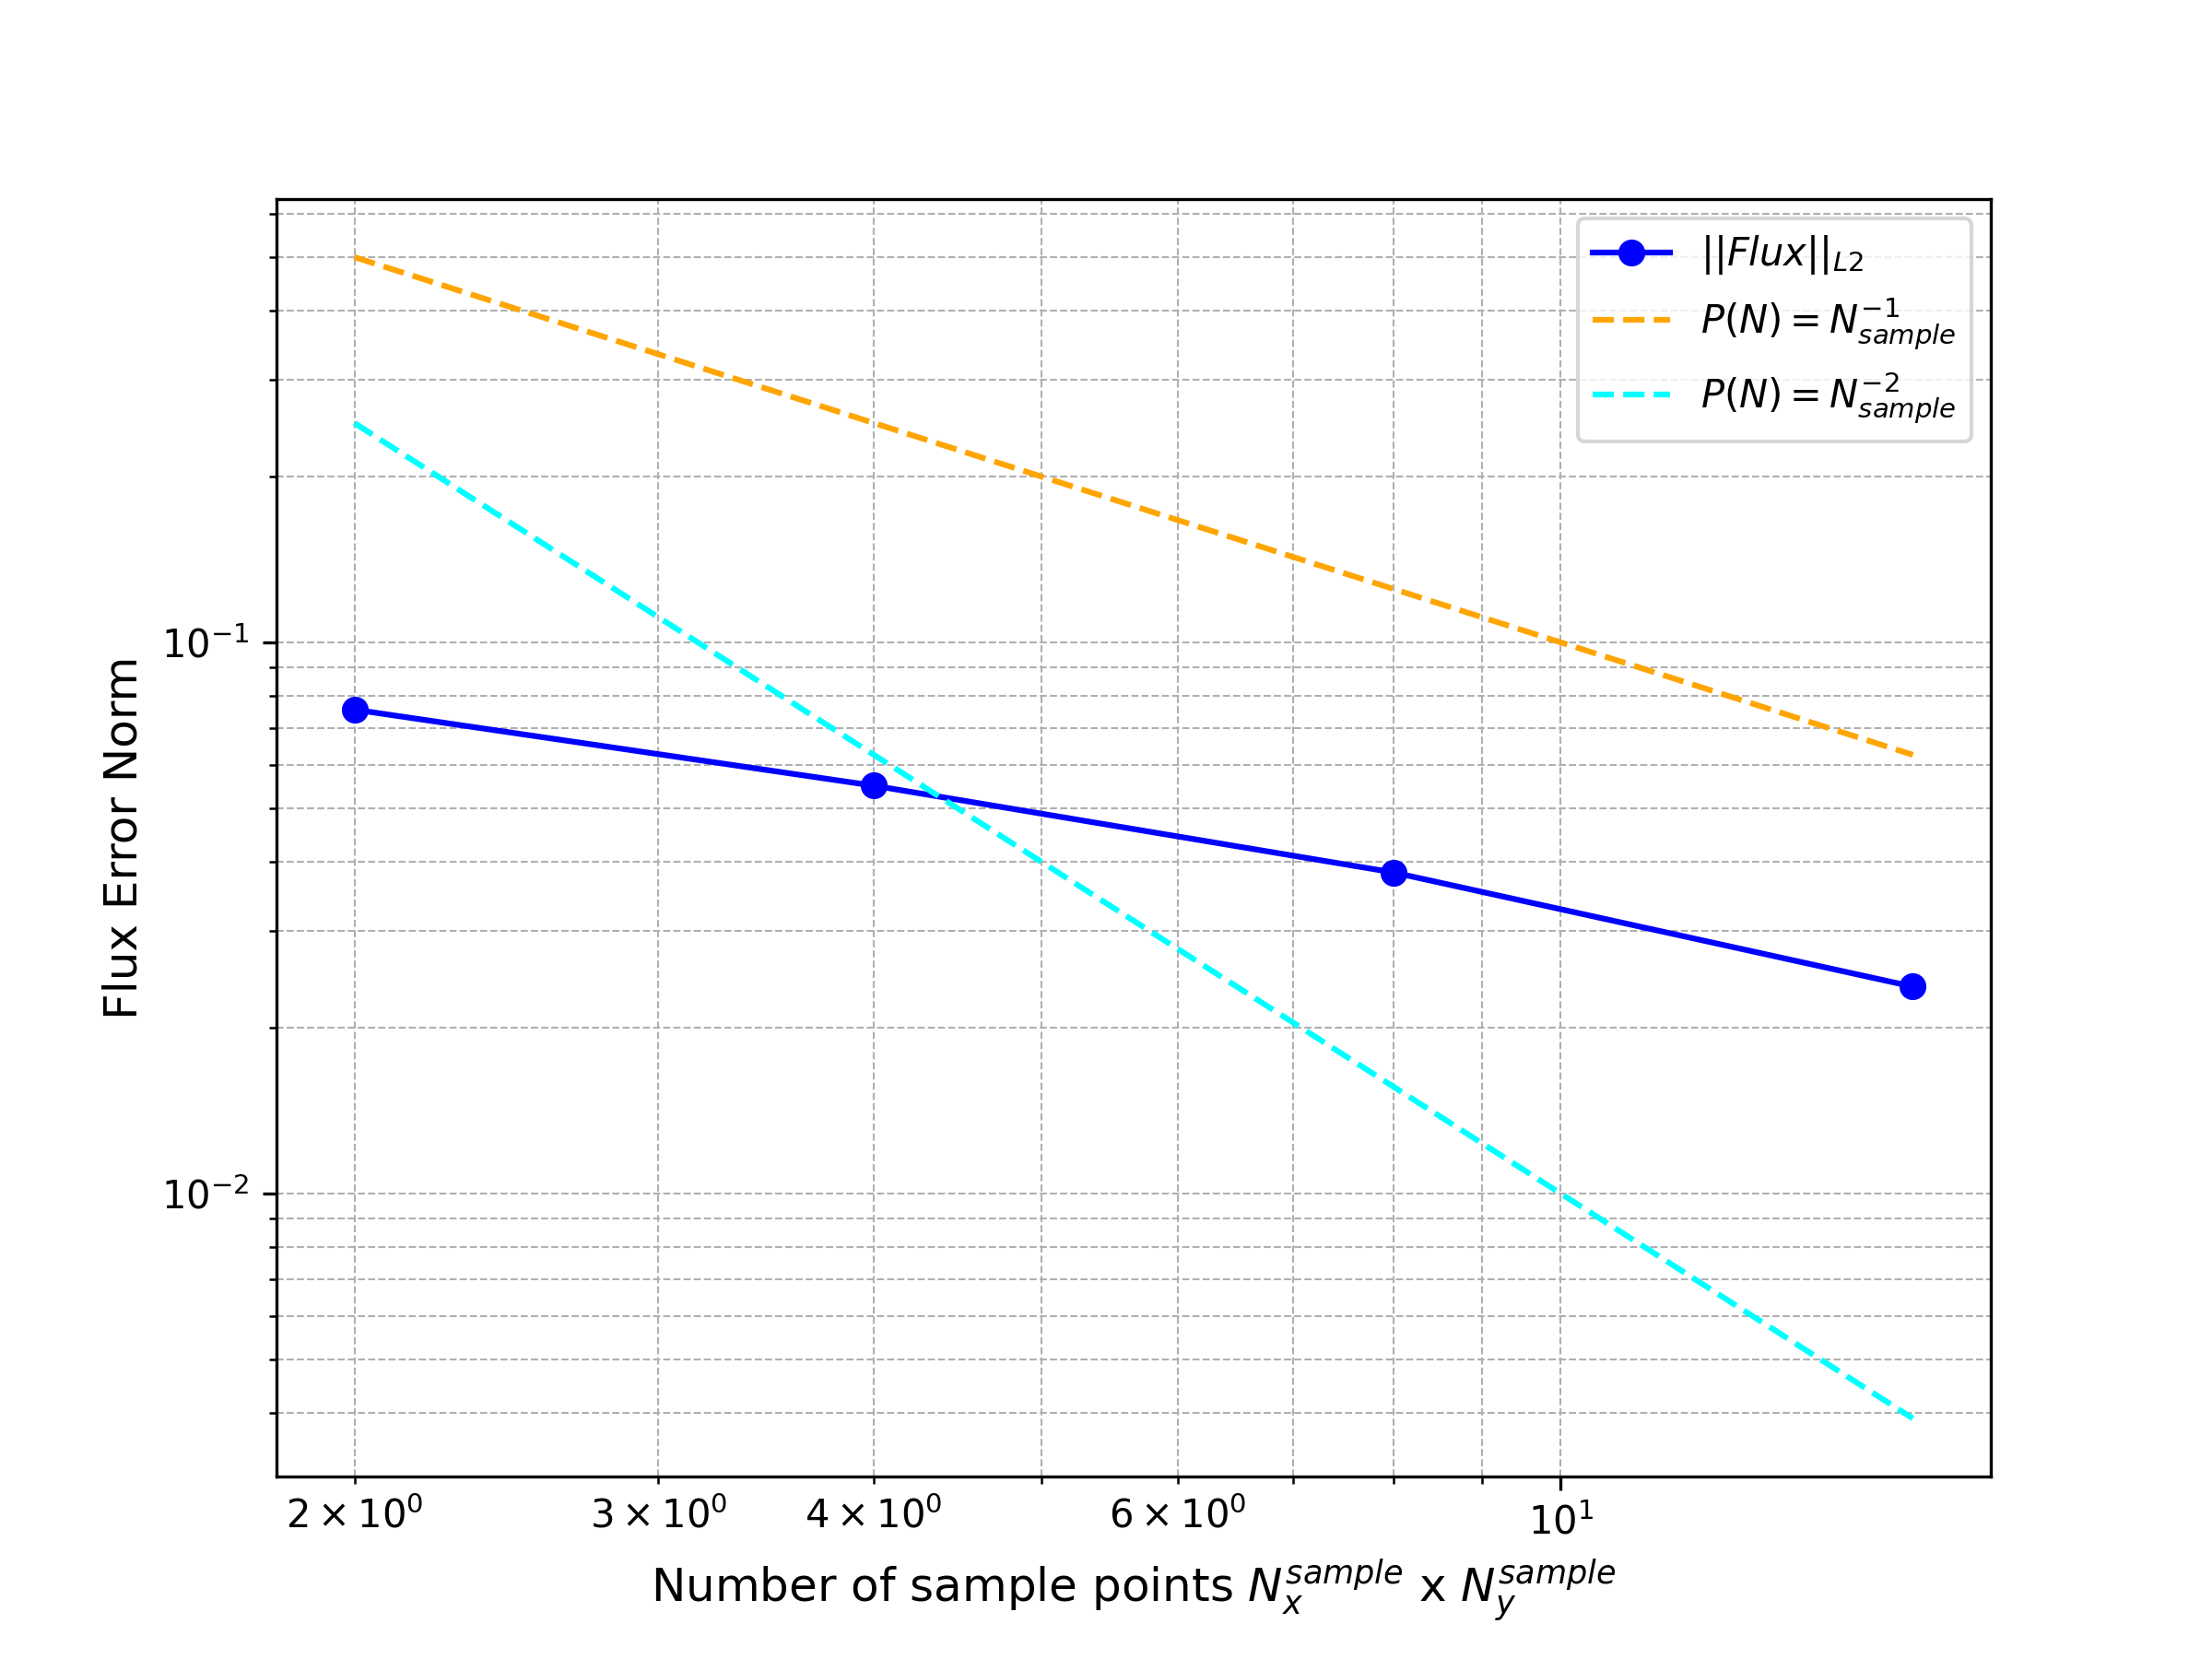
\includegraphics[width=\linewidth]{Figuras/Convergencia_amostras/flux_convergence_Nsample_20_heterogeneous_perm.png}
		\caption{Convergência de $\mathbf{u}$ na norma $L^{2}$.}
		\label{fig:flux_convergence_Nsample_20_heterogeneous_perm}
	\end{subfigure}
	\label{fig:convergence_coarse_mesh_heterogeneous_perm}
\end{figure}

\begin{figure}[!ht]
	\centering
	\caption{Análise de convergência do campo escalar de pressões e do fluxo de Darcy em relação do número de pontos amostrais, em uma malha de elementos finitos $200 \times 200$ e um campo de permeabilidade heterogêneo.}
	\begin{subfigure}[t]{0.45\linewidth}
		\centering
		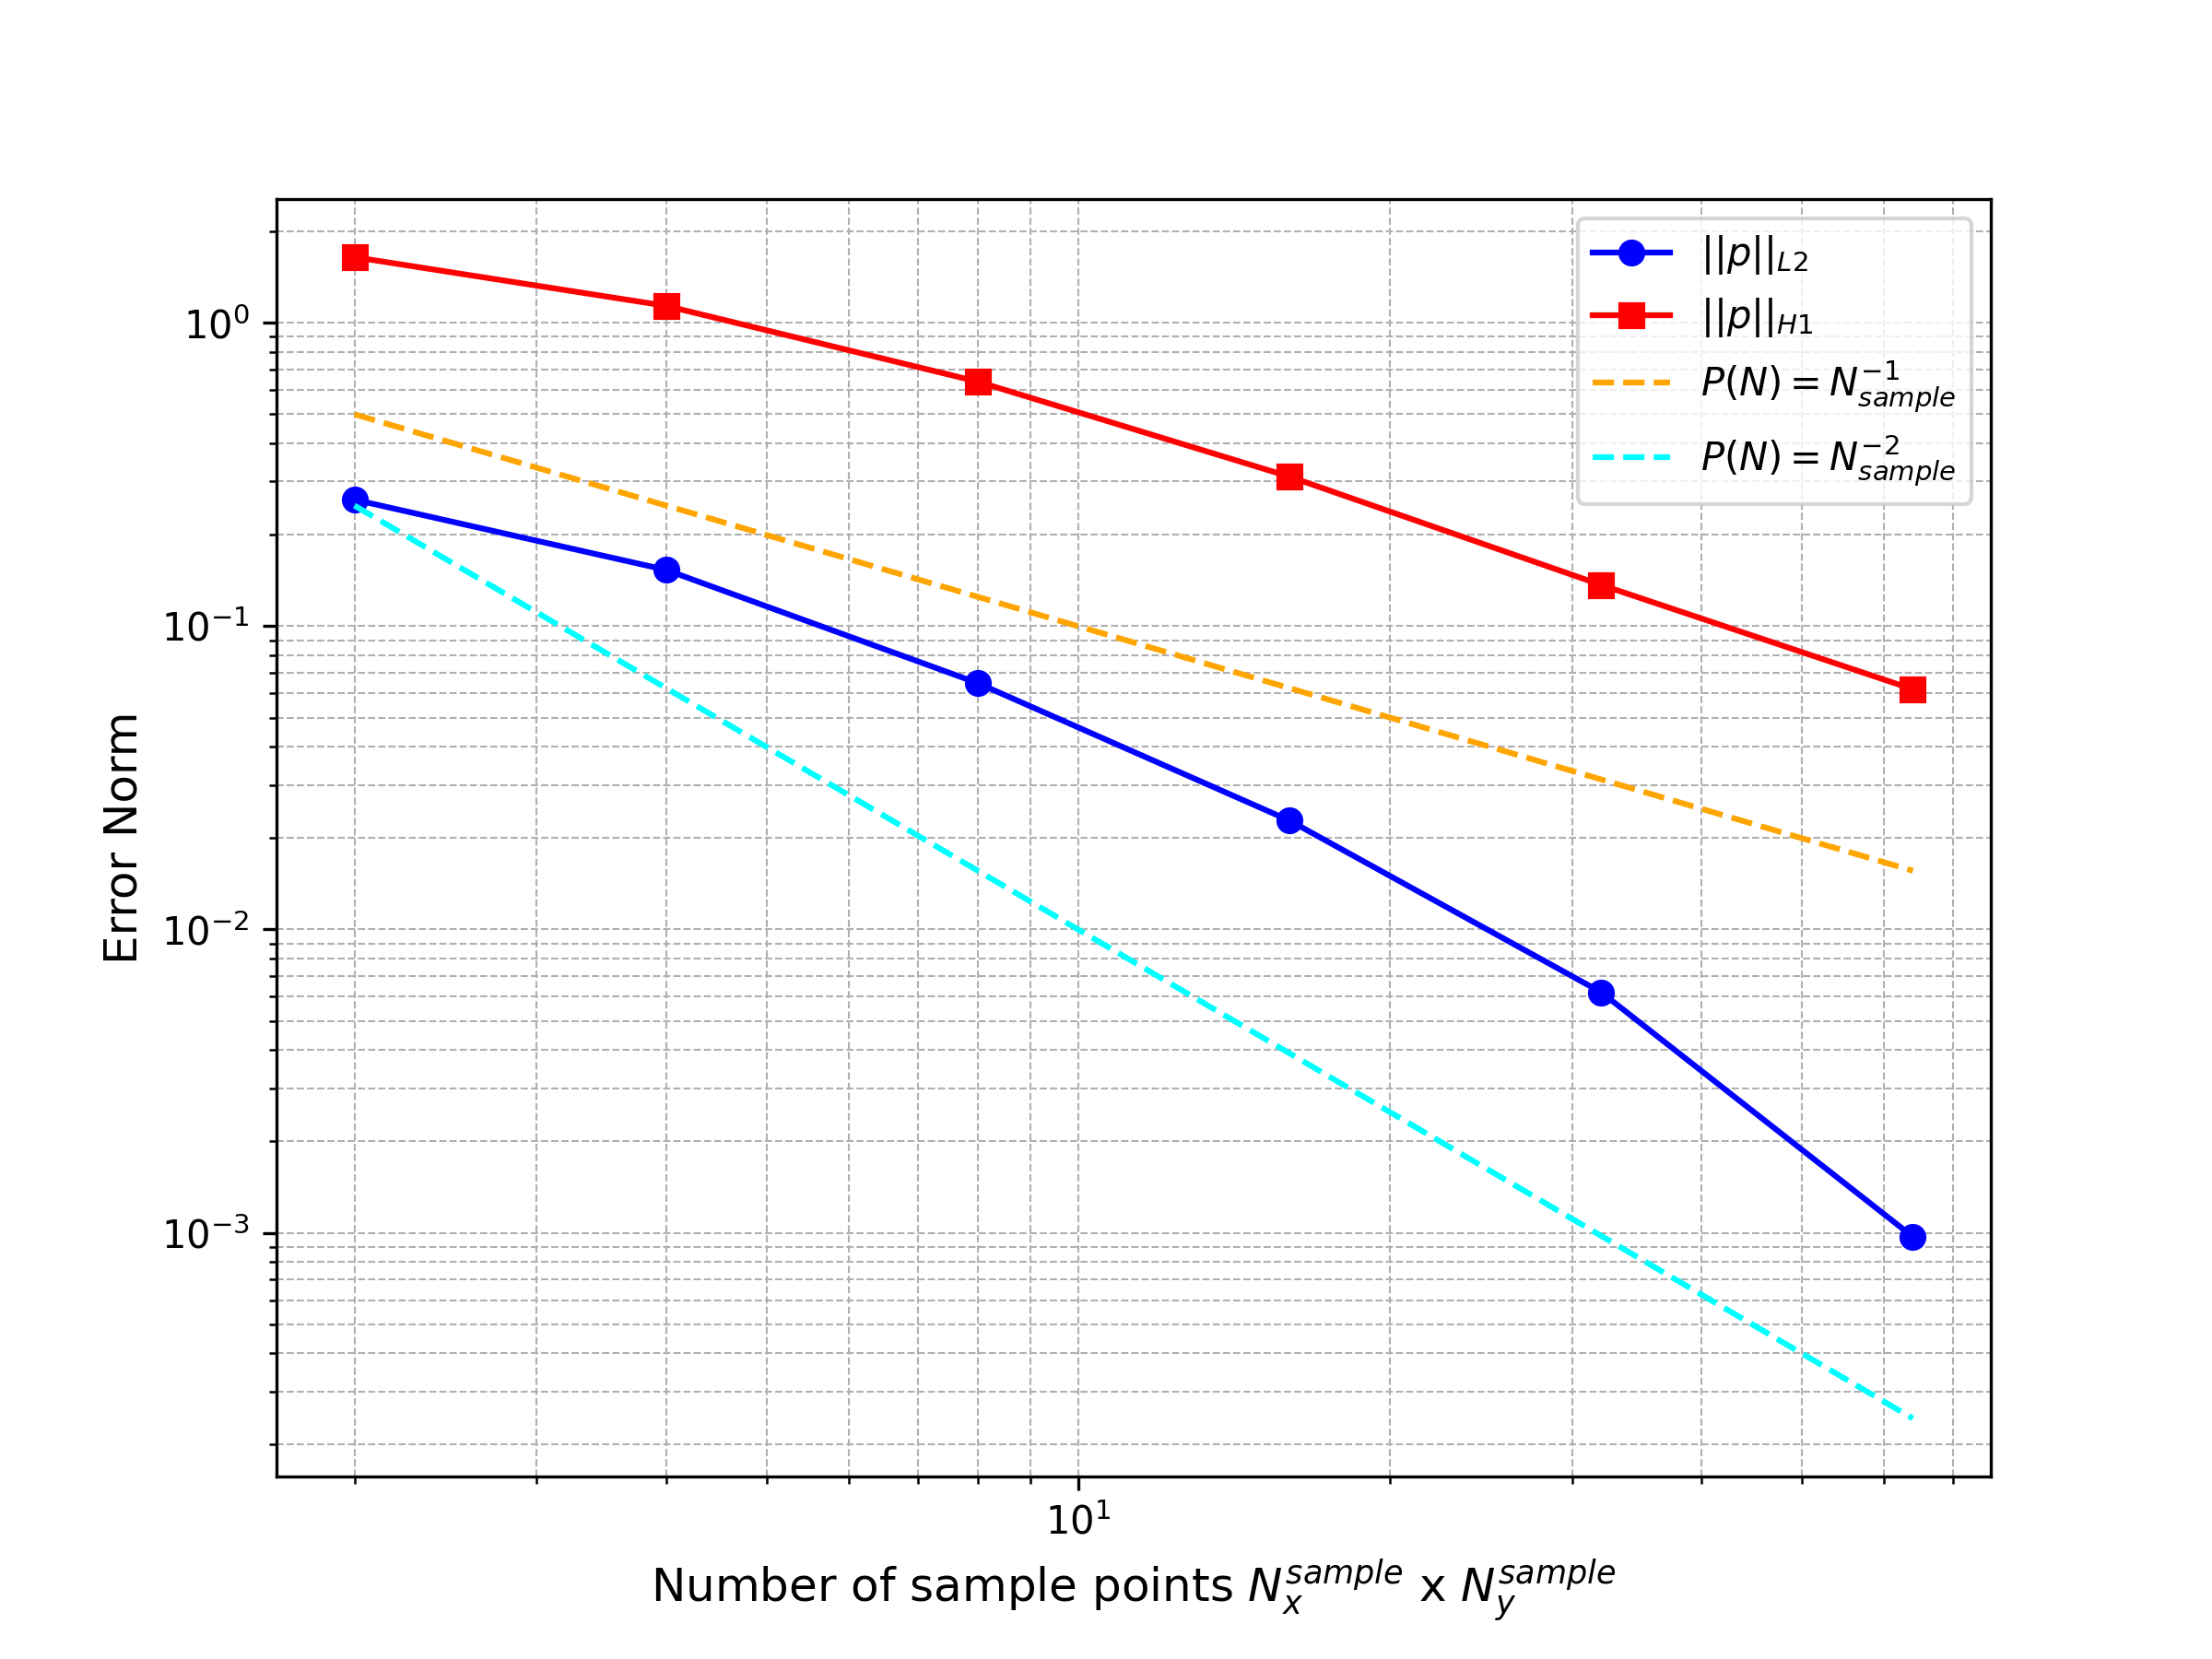
\includegraphics[width=\linewidth]{Figuras/Convergencia_amostras/pressure_convergence_Nsample_200_heterogeneous_perm.png}
		\caption{Convergência de $p$ na norma $L^{2}$ e na norma $H^{1}$.}
		\label{fig:pressure_convergence_Nsample_200_heterogeneous_perm}
	\end{subfigure}
	\begin{subfigure}[t]{0.45\linewidth}
		\centering
		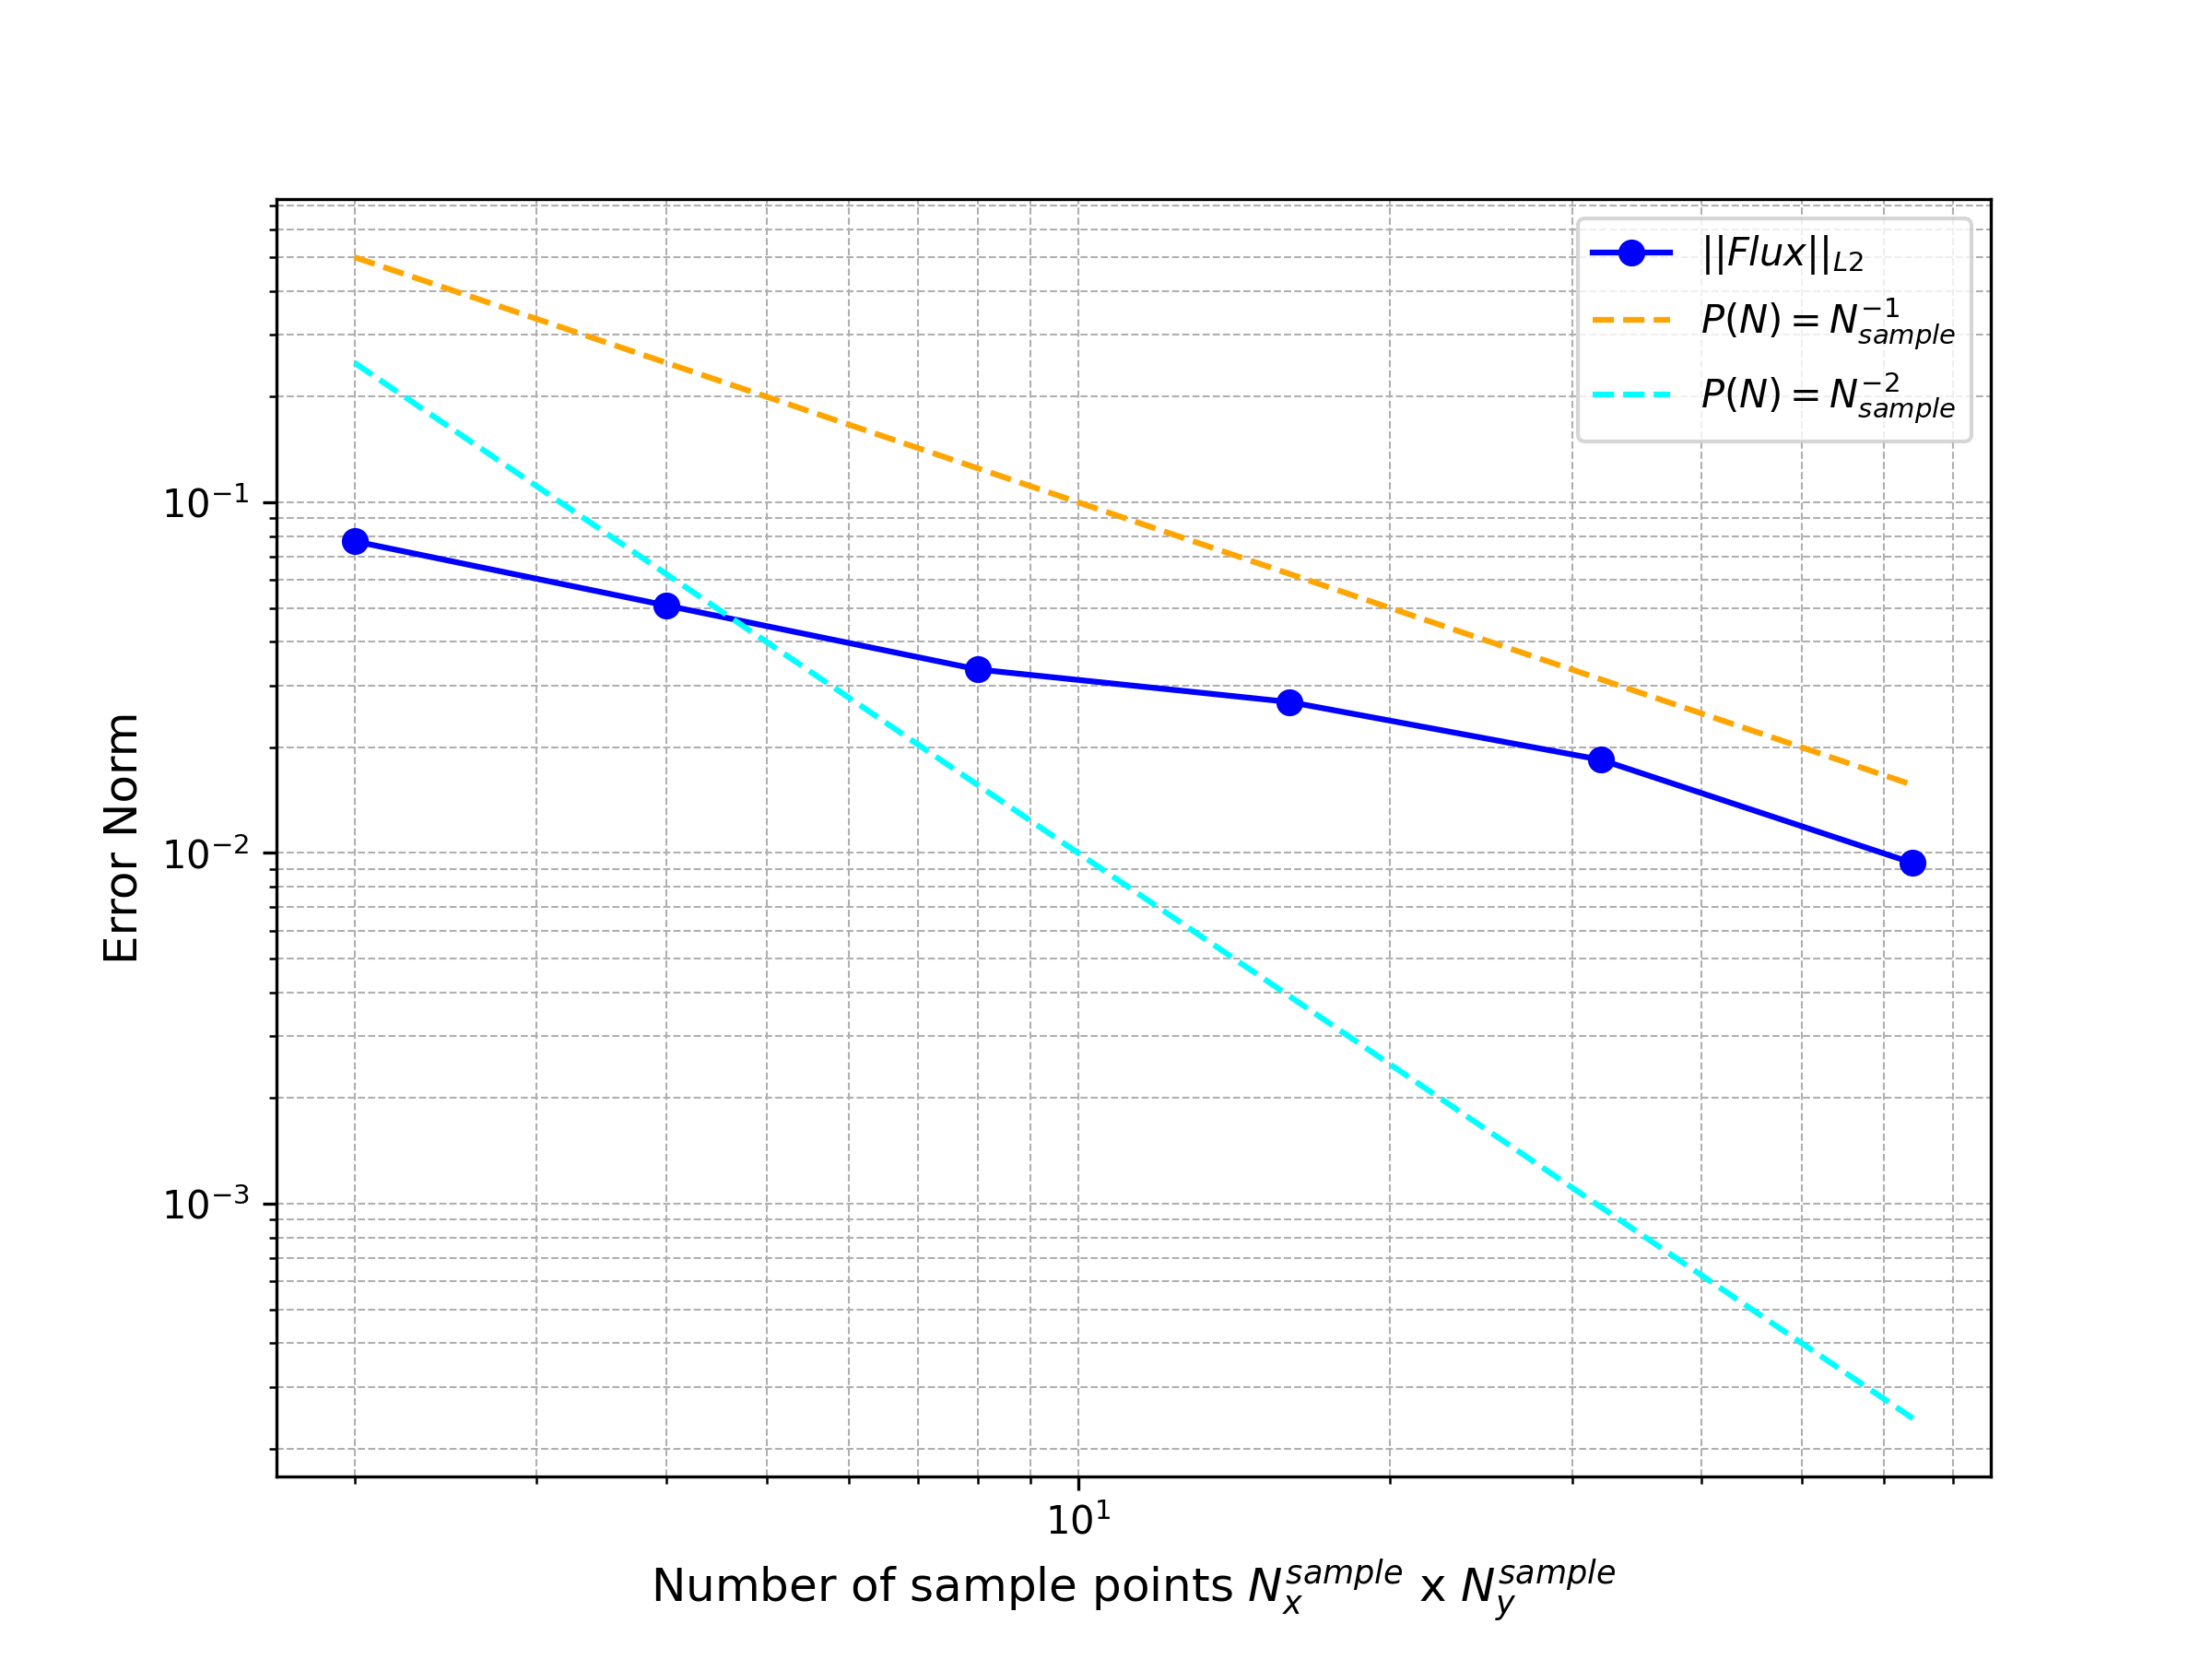
\includegraphics[width=\linewidth]{Figuras/Convergencia_amostras/flux_convergence_Nsample_200_heterogeneous_perm.png}
		\caption{Convergência de $\mathbf{u}$ na norma $L^{2}$.}
		\label{fig:flux_convergence_Nsample_200_heterogeneous_perm}
	\end{subfigure}
	\label{fig:convergence_fine_mesh_heterogeneous_perm}
\end{figure}

\clearpage
\section{Problema de Poisson com condições de contorno mistas}

\begin{equation}
	p(t) = 2(t-0.5), \quad t \in [0,1] \ \text{e} \ (x,y) \in \Gamma_{top}
\end{equation}

\begin{figure}[!ht]
	\centering
	\caption{Campo escalar de pressões para o problema de Poisson com condição de contorno de Dirichlet dependente do tempo.}
	\begin{subfigure}[t]{0.3\linewidth}
		\centering
		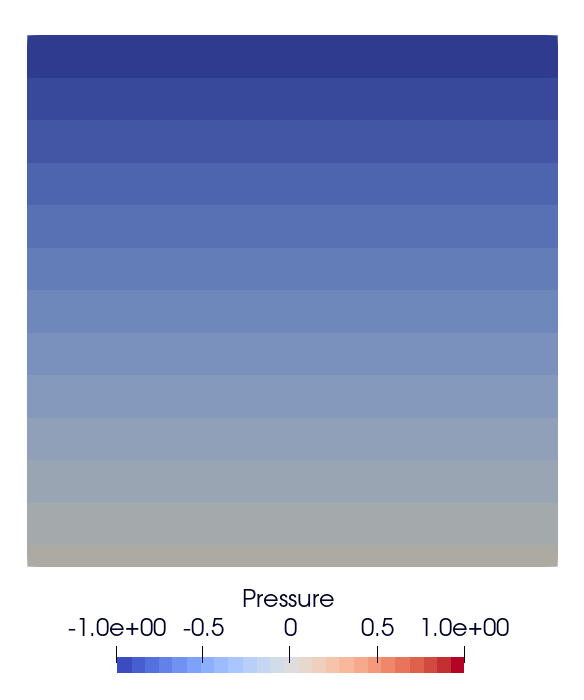
\includegraphics[width=\linewidth]{Figuras/Etapa01/pressure_t0.png}
		\caption{$t=0$.}
		\label{fig:pressure_t0}
	\end{subfigure}
	\begin{subfigure}[t]{0.3\linewidth}
		\centering
		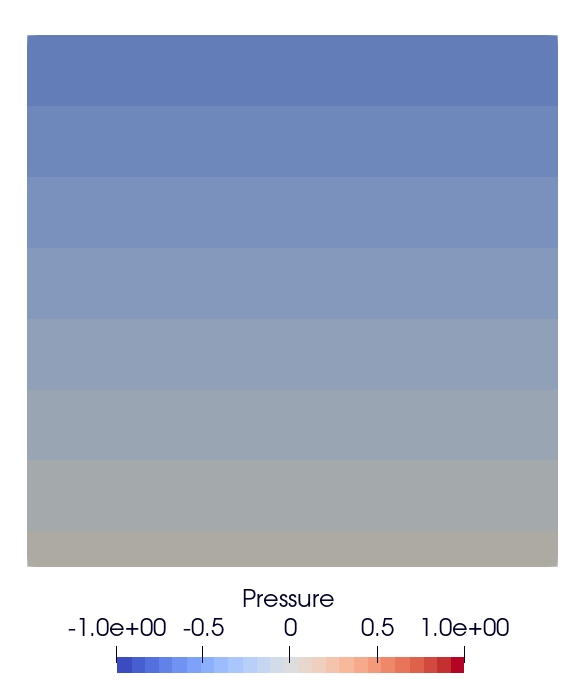
\includegraphics[width=\linewidth]{Figuras/Etapa01/pressure_t2.png}
		\caption{$t = 0.2$.}
		\label{fig:pressure_t1}
	\end{subfigure}
	\begin{subfigure}[t]{0.3\linewidth}
		\centering
		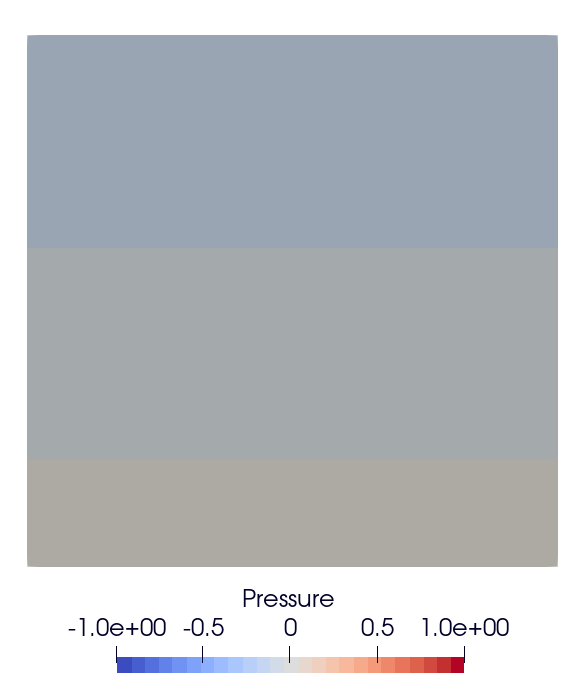
\includegraphics[width=\linewidth]{Figuras/Etapa01/pressure_t4.png}
		\caption{$t = 0.4$.}
		\label{fig:pressure_t2}
	\end{subfigure}
	\begin{subfigure}[t]{0.3\linewidth}
		\centering
		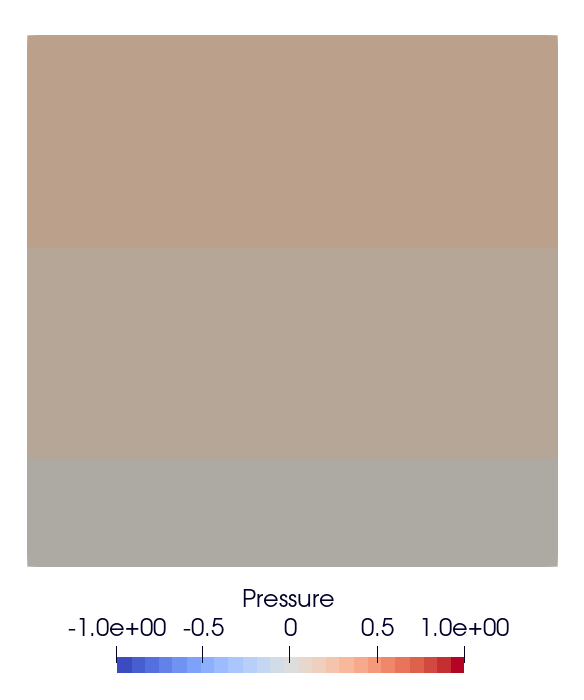
\includegraphics[width=\linewidth]{Figuras/Etapa01/pressure_t6.png}
		\caption{$t = 0.6$.}
		\label{fig:pressure_t4}
	\end{subfigure}
	\begin{subfigure}[t]{0.3\linewidth}
		\centering
		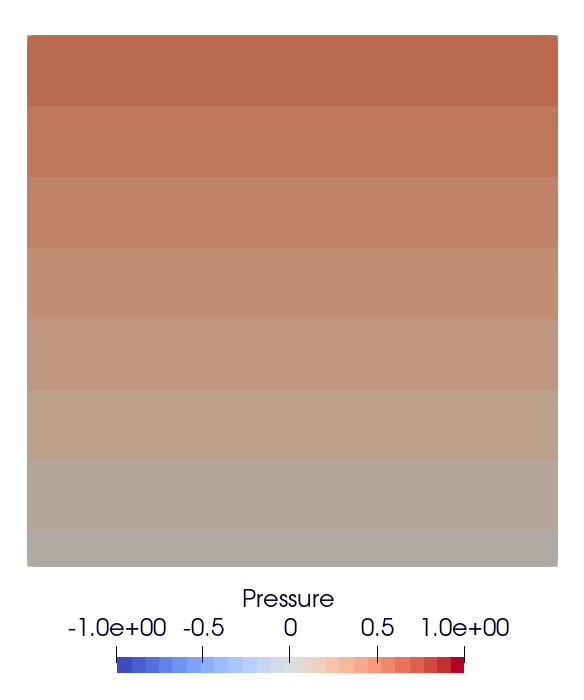
\includegraphics[width=\linewidth]{Figuras/Etapa01/pressure_t8.png}
		\caption{$t = 0.8$.}
		\label{fig:pressure_t5}
	\end{subfigure}
	\begin{subfigure}[t]{0.3\linewidth}
		\centering
		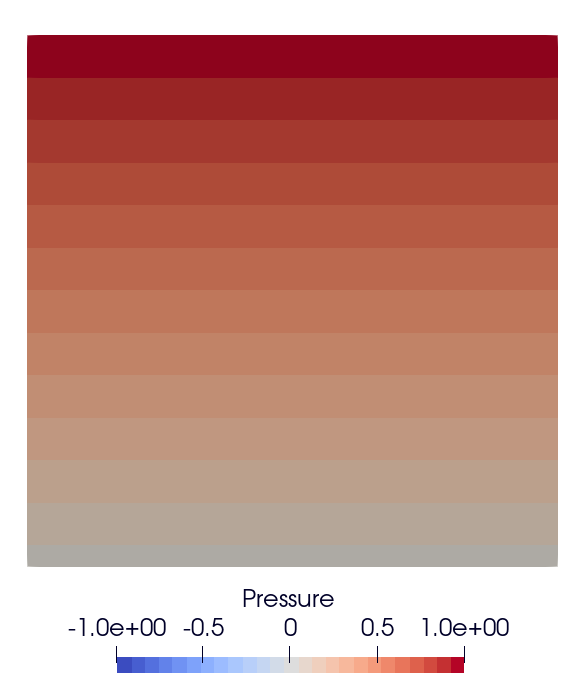
\includegraphics[width=\linewidth]{Figuras/Etapa01/pressure_t10.png}
		\caption{$t = 1.0$.}
		\label{fig:pressure_t6}
	\end{subfigure}
	\label{fig:}
\end{figure}

\begin{figure}[!ht]
	\centering
	\caption{Variação vertical da pressão na coordenada $x=0.5$, em diferentes instantes de tempo.}
	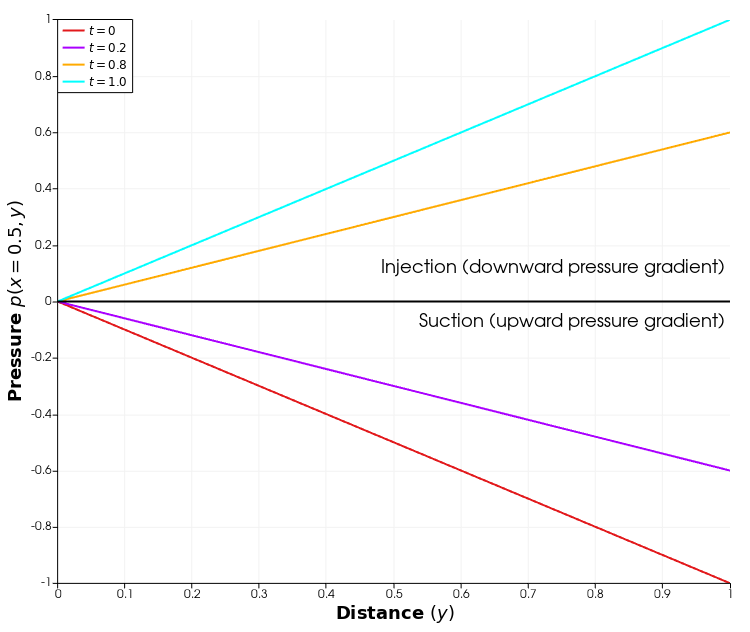
\includegraphics[width = 0.5\linewidth]{Figuras/Etapa01/Poisson_timedependet_bc.png}
	\label{fig:pressure_overline}
\end{figure}




